\documentclass{amsart}[12pt]
\usepackage{graphicx}
\usepackage{comment}
\usepackage{amscd,mathabx}
\usepackage{amssymb,setspace}
\usepackage{tikz-cd}
\usepackage{latexsym,amsfonts,amssymb,amsthm,amsmath,amscd,stmaryrd,mathrsfs,xcolor}
\usepackage[all, knot]{xy}
\usepackage[top=1in, bottom=1in, left=1in, right=1in]{geometry}
\usepackage{imakeidx}
\xyoption{all}
\xyoption{arc}
\usepackage{hyperref}


\newcommand{\qbox}{\tag*{$\blacksquare$}}
%\usepackage[notcite,notref]{showkeys}
 
%\CompileMatricesx
\newcommand{\edit}[1]{\marginpar{\footnotesize{#1}}}
%\newcommand{\edit}[1]{}
\newcommand{\rperf}[2]{\operatorname{RPerf}(#1 \into #2)}



\newcommand{\vectwo}[2]{\begin{bmatrix} #1 \\ #2 \end{bmatrix}}

\newcommand{\vecfour}[4]{\begin{bmatrix} #1 \\ #2 \\ #3 \\ #4 \end{bmatrix}}

\newcommand{\Cat}[1]{\left<\left< \text{#1} \right>\right>}


\def\htpy{\simeq_{\mathrm{htpc}}}
\def\tor{\text{ or }}
\def\fg{finitely generated~}

\def\Ass{\operatorname{Ass}}
\def\ann{\operatorname{ann}}
\def\inc{\operatorname{inc}}
\def\Der{\operatorname{Der}}

\newcommand{\Tor}{\mathrm{Tor}}
\newcommand{\can}{\mathrm{can}}

\def\ob{{\mathfrak{ob}} }
\def\BiAdd{\operatorname{BiAdd}}
\def\BiLin{\operatorname{BiLin}}

\def\Syl{\operatorname{Syl}}
\def\span{\operatorname{span}}

\def\sdp{\rtimes}
\def\cL{\mathcal L}
\def\cR{\mathcal R}



\def\ay{??}
\def\Aut{\operatorname{Aut}}
\def\End{\operatorname{End}}
\def\Mat{\operatorname{Mat}}


\def\a{\alpha}



\def\etale{\'etale~}
\def\tW{\tilde{W}}
\def\tH{\tilde{H}}
\def\tC{\tilde{C}}
\def\tS{\tilde{S}}
\def\tX{\tilde{X}}
\def\tZ{\tilde{Z}}
\def\HBM{H^{\text{BM}}}
\def\tHBM{\tilde{H}^{\text{BM}}}
\def\Hc{H_{\text{c}}}
\def\Hs{H_{\text{sing}}}
\def\cHs{{\mathcal H}_{\text{sing}}}
\newcommand{\htt}{\mathrm{ht}}
\def\Hms{H^{\text{sing}}}
\def\Hm{\Hms}
\def\tHms{\tilde{H}^{\text{sing}}}
\def\Grass{\operatorname{Grass}}
\def\image{\operatorname{im}}
\def\im{\image}
\def\ker{\operatorname{ker}}
\def\coker{\operatorname{coker}}
\def\cone{\operatorname{cone}}
\newcommand{\Hom}{\mathrm{Hom}}
\newcommand{\Spec}{\mathrm{Spec}}

\newcommand{\onto}{\twoheadrightarrow}


\def\ku{ku}
\def\bbu{\bf bu}
\def\KR{K{\mathbb R}}

\def\CW{\underline{CW}}
\def\cP{\mathcal P}
\def\cE{\mathcal E}
\def\cL{\mathcal L}
\def\cJ{\mathcal J}
\def\cJmor{\cJ^\mor}
\def\ctJ{\tilde{\mathcal J}}
\def\tPhi{\tilde{\Phi}}
\def\cA{\mathcal A}
\def\cB{\mathcal B}
\def\cC{\mathcal C}
\def\cZ{\mathcal Z}
\def\cD{\mathcal D}
\def\cF{\mathcal F}
\def\cG{\mathcal G}
\def\cO{\mathcal O}
%\def\cI{\mathcal I}
\def\cS{\mathcal S}
\def\cT{\mathcal T}
\def\cM{\mathcal M}
\def\cN{\mathcal N}
\def\cMpc{{\mathcal M}_{pc}}
\def\cMpctf{{\mathcal M}_{pctf}}
\def\L{\Lambda}

\def\sA{\mathscr A}
\def\sB{\mathscr B}
\def\sC{\mathscr C}
\def\sZ{\mathscr  Z}
\def\sD{\mathscr  D}
\def\sF{\mathscr  F}
\def\sG{\mathscr G}
\def\sO{\mathscr  O}
\def\sI{\mathscr I}
\def\sS{\mathscr S}
\def\sT{\mathscr  T}
\def\sM{\mathscr M}
\def\sN{\mathscr N}

%\newcommand{\inc}{\subseteq}
\newcommand{\id}{\mathrm{id}}


\newcommand{\Jan}[1]{\textcolor{violet}{Lecture of January #1, 2023}}
\newcommand{\Feb}[1]{\textcolor{violet}{Lecture of February #1, 2023}}
\newcommand{\Mar}[1]{\textcolor{violet}{Lecture of March #1, 2023}}
\newcommand{\Apr}[1]{\textcolor{violet}{Lecture of April #1, 2023}}
\newcommand{\May}[1]{\textcolor{violet}{Lecture of May #1, 2023}}

\def\Ext{\operatorname{Ext}}
 \def\ext{\operatorname{ext}}



\def\ov#1{{\overline{#1}}}

\def\vecthree#1#2#3{\begin{bmatrix} #1 \\ #2 \\ #3 \end{bmatrix}}

\def\tOmega{\tilde{\Omega}}
\def\tDelta{\tilde{\Delta}}
\def\tSigma{\tilde{\Sigma}}
\def\tsigma{\tilde{\sigma}}


\newcommand{\bs}[1]{\mathbf{#1}}

\def\d{\delta}
\def\td{\tilde{\delta}}

\def\e{\epsilon}
\def\nsg{\unlhd}
\def\pnsg{\lhd}

\newcommand{\tensor}{\otimes}
\newcommand{\homotopic}{\simeq}
\newcommand{\homeq}{\cong}
\newcommand{\iso}{\approx}

\DeclareMathOperator{\ho}{Ho}
\DeclareMathOperator*{\colim}{colim}


\newcommand{\Q}{\mathbb{Q}}
\renewcommand{\H}{\mathbb{H}}

\newcommand{\bP}{\mathbb{P}}
\newcommand{\bM}{\mathbb{M}}
\newcommand{\A}{\mathbb{A}}
\newcommand{\bH}{{\mathbb{H}}}
\newcommand{\G}{\mathbb{G}}
\newcommand{\bR}{{\mathbb{R}}}
\newcommand{\bL}{{\mathbb{L}}}
\newcommand{\R}{{\mathbb{R}}}
\newcommand{\F}{\mathbb{F}}
\newcommand{\E}{\mathbb{E}}
\newcommand{\bF}{\mathbb{F}}
\newcommand{\bE}{\mathbb{E}}
\newcommand{\bK}{\mathbb{K}}


\newcommand{\bD}{\mathbb{D}}
\newcommand{\bS}{\mathbb{S}}

\newcommand{\bN}{\mathbb{N}}


\newcommand{\bG}{\mathbb{G}}

\newcommand{\C}{\mathbb{C}}
\newcommand{\Z}{\mathbb{Z}}
\newcommand{\N}{\mathbb{N}}

\newcommand{\M}{\mathcal{M}}
\newcommand{\W}{\mathcal{W}}



\newcommand{\itilde}{\tilde{\imath}}
\newcommand{\jtilde}{\tilde{\jmath}}
\newcommand{\ihat}{\hat{\imath}}
\newcommand{\jhat}{\hat{\jmath}}

\newcommand{\fc}{{\mathfrak c}}
\newcommand{\fp}{{\mathfrak p}}
\newcommand{\fm}{{\mathfrak m}}
\newcommand{\fn}{{\mathfrak n}}
\newcommand{\fq}{{\mathfrak q}}
\newcommand{\fr}{{\mathfrak r}}

\newcommand{\op}{\mathrm{op}}
\newcommand{\dual}{\vee}

\newcommand{\DEF}[1]{\emph{#1}\index{#1}}
\newcommand{\Def}[1]{#1 \index{#1}}


% The following causes equations to be numbered within sections
\numberwithin{equation}{section}


\theoremstyle{plain} %% This is the default, anyway
\newtheorem{thm}[equation]{Theorem}
\newtheorem{thmdef}[equation]{TheoremDefinition}
\newtheorem{introthm}{Theorem}
\newtheorem{introcor}[introthm]{Corollary}
\newtheorem*{introthm*}{Theorem}
\newtheorem{question}{Question}
\newtheorem{cor}[equation]{Corollary}
\newtheorem{por}[equation]{Porism}
\newtheorem{lem}[equation]{Lemma}
\newtheorem{lemminition}[equation]{Lemminition}
\newtheorem{prop}[equation]{Proposition}
\newtheorem{porism}[equation]{Porism}
\newtheorem{fact}[equation]{Fact}


\newtheorem{conj}[equation]{Conjecture}
\newtheorem{quest}[equation]{Question}

\theoremstyle{definition}
\newtheorem{defn}[equation]{Definition}
\newtheorem{chunk}[equation]{}
\newtheorem{ex}[equation]{Example}

\newtheorem{exer}[equation]{Optional Exercise}

\theoremstyle{remark}
\newtheorem{rem}[equation]{Remark}

\newtheorem{notation}[equation]{Notation}
\newtheorem{terminology}[equation]{Terminology}



\renewcommand{\sec}[1]{\section{#1}}
\newcommand{\ssec}[1]{\subsection{#1}}
\newcommand{\sssec}[1]{\subsubsection{#1}}

\newcommand{\br}[1]{\lbrace \, #1 \, \rbrace}
\newcommand{\li}{ < \infty}
\newcommand{\quis}{\simeq}
\newcommand{\xra}[1]{\xrightarrow{#1}}
\newcommand{\xla}[1]{\xleftarrow{#1}}
\newcommand{\xlra}[1]{\overset{#1}{\longleftrightarrow}}

\newcommand{\xroa}[1]{\overset{#1}{\twoheadrightarrow}}
\newcommand{\xria}[1]{\overset{#1}{\hookrightarrow}}
\newcommand{\ps}[1]{\mathbb{P}_{#1}^{\text{c}-1}}




\def\and{{ \text{ and } }}
\def\oor{{ \text{ or } }}

\def\Perm{\operatorname{Perm}}
\newcommand{\Ss}{\mathbb{S}}

\def\Op{\operatorname{Op}}
\def\res{\operatorname{res}}
\def\ind{\operatorname{ind}}

\def\sign{{\mathrm{sign}}}
\def\naive{{\mathrm{naive}}}
\def\l{\lambda}


\def\ov#1{\overline{#1}}
\def\cV{{\mathcal V}}
%%%-------------------------------------------------------------------
%%%-------------------------------------------------------------------

\newcommand{\chara}{\operatorname{char}}
\newcommand{\Kos}{\operatorname{Kos}}
\newcommand{\opp}{\operatorname{opp}}
\newcommand{\perf}{\operatorname{perf}}

\newcommand{\Fun}{\operatorname{Fun}}
\newcommand{\GL}{\operatorname{GL}}
\newcommand{\SL}{\operatorname{SL}}
\def\o{\omega}
\def\oo{\overline{\omega}}

\def\cont{\operatorname{cont}}
\def\te{\tilde{e}}
\def\gcd{\operatorname{gcd}}

\def\stab{\operatorname{stab}}

\def\va{\underline{a}}

\def\ua{\underline{a}}
\def\ub{\underline{b}}


\newcommand{\Ob}{\mathrm{Ob}}
\newcommand{\Set}{\mathbf{Set}}
\newcommand{\Grp}{\mathbf{Grp}}
\newcommand{\Ab}{\mathbf{Ab}}
\newcommand{\Sgrp}{\mathbf{Sgrp}}
\newcommand{\Ring}{\mathbf{Ring}}
\newcommand{\Fld}{\mathbf{Fld}}
\newcommand{\cRing}{\mathbf{cRing}}
\newcommand{\Mod}[1]{#1-\mathbf{Mod}}
\newcommand{\Cx}[1]{#1-\mathbf{Comp}}
\newcommand{\vs}[1]{#1-\mathbf{vect}}
\newcommand{\Vs}[1]{#1-\mathbf{Vect}}
\newcommand{\vsp}[1]{#1-\mathbf{vect}^+}
\newcommand{\Top}{\mathbf{Top}}
\newcommand{\Setp}{\mathbf{Set}_*}
\newcommand{\Alg}[1]{#1-\mathbf{Alg}}
\newcommand{\cAlg}[1]{#1-\mathbf{cAlg}}
\newcommand{\PO}{\mathbf{PO}}
\newcommand{\Cont}{\mathrm{Cont}}
\newcommand{\MaT}[1]{\mathbf{Mat}_{#1}}
\newcommand{\Rep}[2]{\mathbf{Rep}_{#1}(#2)}
\newcommand{\Holo}{\mathrm{Holo}}

\newcommand{\red}[1]{{\color{red}#1}}
\newcommand{\blue}[1]{{\color{blue}#1}}

%%%-------------------------------------------------------------------
%%%-------------------------------------------------------------------
%%%-------------------------------------------------------------------
%%%-------------------------------------------------------------------
%%%-------------------------------------------------------------------

\makeindex
\title{Math 918 Lecture Notes, Spring 2023}


\begin{document}
\onehalfspacing

\maketitle

%\tableofcontents


\Jan{24}

\sec{Derivations}

\ssec{Definition and first examples}


Our goal will be to consider derivatives algebraically.

The usual notion of derivative of a function is a rule that turns certain real-valued or complex-valued functions into other real-valued or complex-valued functions as follows: at a given point $x$, we take
\[ f'(x) = \lim_{y\to x} \frac{f(y)-f(x)}{y-x}.\]
This certainly gives us derivative functions on some rings, for example,
the ring of infinitely-differentiable functions on $\R$:\index{infinitely-differentiable functions on $\R$}\index{$\cC^{\infty}(\R)$}
\[  \cC^{\infty}(\R) \xra{\frac{d}{dx}} \cC^{\infty}(\R)\]
or the ring of \emph{entire functions}\index{entire}, i.e., \emph{holomorphic}\index{holomorphic}, a.k.a. complex-differentiable, functions on the complex plane\index{$\Holo(\C)$}:
\[ \Holo(\C) \xra{\frac{d}{dx}}\Holo(\C). \]
Neither of these is the sort of ring that we usually consider in commutative algebra. In particular, neither is Noetherian.

Using our familiar rules of differentiation, we might recall that the derivative of a polynomial is a polynomial, and the derivative of a rational function is a rational function. So, we get derivatives on much more manageable rings:
\[ \R[x] \xra{\frac{d}{dx}} \R[x], \quad \R(x) \xra{\frac{d}{dx}} \R(x), \quad \C[x] \xra{\frac{d}{dx}} \C[x], \quad \C(x) \xra{\frac{d}{dx}} \C(x).\]

To unlock some of the applications of derivatives, we would like to be able to do this as much as possible over arbitrary rings. We might be optimistic about doing this for arbitrary polynomial rings at least, given the examples above. To do it, we certainly must get rid of this limit approach, since moving around in fields like $\Q$ or $\F_p$ we certainly will miss out on lots of limits. Of course, when we actually compute the derivative of a real or complex polynomial, we don't consider the limit definition anymore, but instead use rules of derivative. Namely, we have a sum rule, a scalar rule, a product rule, a quotient rule, and a power rule, and knowing all of these, we easily and limitlessly compute derivatives of any polynomial or rational function over $\R$ or $\C$. Since the quotient rule and power rule (mostly) follow from the product rule, we will hone in on the first three for our definition of algebraic notion of derivative.

So, our first approximation of the definition of \emph{derivation}, our notion of derivative, is a function $\partial$ from a ring $R$ to itself that satisfies a sum rule, a scalar rule, and a product rule:
\begin{itemize}
\item $\partial(r+s) = \partial(r)+\partial(s)$ for all $r,s\in R$,
\item $\partial(cr)= c\partial(r)$ for all $r\in R$ and $c$ ``constant???",
\item $\partial(rs) = r\partial(s) + s\partial(r)$ for all $r,s\in R$.
\end{itemize}

There is something we must change (``constant???") and something else less clear we can/should change. Let's be openminded. If $R$ is a ring, let's let our constants be any reasonable set of elements of $R$: any subring $A$ of $R$. But let's be even more openminded. Look at the right-hand sides above. To make sense of them we have to be able to add our outputs together and multiply them by ring elements, but we don't have to multiply them with each other. They don't have to live in $R$---they just have to live in an $R$-module.

\begin{defn} Let $R$ be a ring and $M$ be an $R$-module. A \emph{derivation}\index{derivation} from $R$ to $M$ is a function $\partial:R\to M$ such that
\begin{itemize}
\item $\partial(r+s) = \partial(r) + \partial(s)$ for all $r,s\in R$,
\item $\partial(rs) = r\partial(s) + s\partial(r)$ for all $r,s\in R$.
\end{itemize}
If $R$ is an $A$-algebra, then $\partial$ is a \emph{derivation over $A$}\index{derivation over $A$} or an \emph{$A$-linear derivation}\index{$A$-linear derivation} if in addition
\begin{itemize}
\item $\partial(ar) = a \partial(r)$ for all $a\in A$ and $r\in R$.
\end{itemize}
\end{defn}

\begin{rem} Recall that $R$ is an $A$-algebra means that $R$ is equipped with a ring homomorphism $\phi:A\to R$. In this case, every $R$-module is also an $A$-module by restriction of scalars: $a  m := \phi(a) m$; i.e., for $A$ to act on $M$, just view elements of $A$ as elements of $R$ via $\phi$ and do the same action. This is what's going on in the right-hand side above. We'll circle back to restriction of scalars soon.
\end{rem}

\sssec{Examples of derivations}

Let's consider some examples of derivations to buy into this notion. 


First, let's construct the ``usual derivative'' for a polynomial or a power series ring, and show it is a derivation.

\begin{defn}
Let $A$ be a ring and $R=A[x]$ a polynomial ring. We define $\frac{d}{dx}:R\to R$ by the rule
\[ \frac{d}{dx} ( \sum_{j=0}^d a_j x^j) = \sum_{j=1}^d j a_j x^{j-1}.\]\index{$\frac{d}{dx}$}
Similarly, for a power series ring, $R= A\llbracket x\rrbracket$, we define
$\frac{d}{dx}:R\to R$ by the rule
\[ \frac{d}{dx} ( \sum_{j=0}^\infty a_j x^j) = \sum_{j=1}^\infty j a_j x^{j-1}.\]
\end{defn}


\begin{lem}
The functions $\frac{d}{dx}: A[x] \to A[x]$ and $\frac{d}{dx}: A\llbracket x\rrbracket \to  A\llbracket x\rrbracket$ are $A$-linear derivations.
\end{lem}
\begin{proof}
In either case, we have a well-defined function returning an object of the same type. The formulas are the same in both cases, just allowing infinite formal sums for power series, so we'll deal with both simultaneously. 

Take $r= \sum_{j=0} a_j x^j$, $s= \sum_{j=0} b_j x^j$, and $c$ with $a_j,b_j,c\in A$. Then
\[ \frac{d}{dx} (r+s) = \frac{d}{dx}  (\sum_{j=0} (a_j+b_j) x^j ) = \sum_{j=1} j (a_j+b_j) x^{j-1} = \frac{d}{dx}(r) + \frac{d}{dx}(s),\]
\[ \frac{d}{dx} (cr) = \frac{d}{dx}  (\sum_{j=0} (ca_j) x^j ) = \sum_{j=1} j (ca_j) x^{j-1} = c \frac{d}{dx}(r) ,\]
and
\[\begin{aligned}
 r\frac{d}{dx}(s) + s \frac{d}{dx}(r) &= (\sum_{i=0} a_i x^i )( \sum_{j=1} j b_j x^{j-1}) + (\sum_{j=0} b_j x^j )( \sum_{i=1} i a_i x^{i-1}) 
 \\ &= \sum_{k=1} \sum_{i+j=k} (a_i j b_j) x^{i+j-1} + \sum_{k=1} \sum_{i+j=k} (i a_i b_j) x^{i+j-1} 
 \\&= \sum_{k=1} \sum_{i+j=k} k a_i b_j x^{i+j-1} 
 \\&= \frac{d}{dx}  (\sum_{k=0} \sum_{i+j=k} (a_ib_j) x^k ) = \frac{d}{dx} (rs). \qedhere
\end{aligned}\]
 \end{proof}
 

Note that we could have written the formula above as $\frac{d}{dx} ( \sum_{j=0}^d a_j x^j) = \sum_{j=1}^d j a_j x^{j-1}$ as well: it looks like we have something illegal when $j=0$, but the coefficient of zero tells us to ignore it.

\begin{prop}
Let $A$ be a ring, $\{X_\lambda \  | \ \lambda\in \Lambda\}$, and $R=A[X_\lambda \  | \ \lambda\in \Lambda]$ be a polynomial ring. Then the partial derivatives $\frac{d}{d X_\lambda}$ given by the rule
\[ \frac{d}{dx_\lambda} ( \sum_{\alpha} a_\alpha X^{\alpha}) = \sum_{\alpha} \alpha_\lambda a_\alpha X^{\alpha-e_\lambda}\]\index{$\frac{d}{dx_\lambda}$}where $\alpha\in \N^{\Lambda}$ is an exponent tuple and $e_\lambda$ is the unit vector in the $\lambda$ coordinate,
are $A$-linear derivations. Similarly for the power series ring $R=A\llbracket X_\lambda \  | \ \lambda\in \Lambda\rrbracket$.
\end{prop}
\begin{proof}
Consider $R$ as $R'[X_\lambda]$, with $R'=A[X_\mu \ | \ \mu\in \Lambda\smallsetminus \{\lambda\}]$. Then $\frac{d}{d X_\lambda}$ is just the ``usual derivative'' in this polynomial ring over $R'$, so it is an $R'$-linear derivation of $R$. But since $A\subseteq R'$, this is an $A$-linear derivation as well.
\end{proof}



So we can differentiate over any polynomial ring now, e.g., over $R=\F_2[x]$. Let's not neglect our original derivatives.

\begin{ex}
The standard derivatives
\[  \cC^{\infty}(\R) \xra{\frac{d}{dx}} \cC^{\infty}(\R)\]
and 
\[ \Holo(\C) \xra{\frac{d}{dx}}\Holo(\C) \]
are $\R$-linear and $\C$-linear derivations, respectively.
\end{ex}

We haven't seen examples where we take derivations into ``actual'' modules yet. It turns out that this is a natural thing to do. In fact, examples like this appear in calculus before derivations back into the ring!

\begin{ex}
Let's return to old-fashioned derivatives of $\C^\infty$ functions. Before we get derivatives of functions as functions, we start with the notion of derivative at a point, which should just be a number. Let's try to realize ``derivative at $x=x_0$'' for some real number $x_0$, which we'll write as $\frac{d}{dx}|_{x=x_0}$\index{derivative at $x=x_0$}, as a derivation on $\cC^{\infty}(\R)$. \index{${\frac{d}{dx}}\mid_{x=x_0}$}
The target should be $\R$:
\[ \frac{d}{dx}|_{x=x_0} : \cC^{\infty}(\R) \to \R,\]
so we need to view $\R$ as a $\cC^{\infty}(\R)$-module. A very $x=x_0$ flavored way of doing so is by the rule
\[ f \cdot c = f(x_0) c.\]
Another useful way of thinking about this module structure is as the quotient $\cC^{\infty}(\R)/\fm_{x_0}$, where $\fm_{x_0}$ is the maximal ideal consisting of functions with $f(x_0)=0$. Indeed, the evaluation at $0$ map
\[ \mathrm{ev}_{x_0}  \cC^{\infty}(\R) \to \R\]
has kernel $\fm_{x_0}$ by definition, and if $\R$ has the module structure given above, this map is $\cC^{\infty}(\R)$-linear: if $f\in  \cC^{\infty}(\R)$ and $c\in \R$, then $\mathrm{ev}_{x_0}(fc) = f(x_0) c = f\cdot c$. Of course, if $x_0$ changed, we would get a different module structure.

Back to our derivative. Take $f,g\in \cC^{\infty}(\R)$ and $c\in \R$. Note that this $c$ is an element of $\R \subseteq \cC^{\infty}(\R)$ as opposed to $\R\cong \cC^{\infty}(\R)/\fm_{x_0}$. Then
\[  \frac{d}{dx}|_{x=x_0}\ (f+g) = \frac{d}{dx}|_{x=x_0}\ f + \frac{d}{dx}|_{x=x_0} \ g\]
\[ \frac{d}{dx}|_{x=x_0}\ cf = c \frac{d}{dx}|_{x=x_0}\ f \]
and by the product rule
\[ \frac{d}{dx}|_{x=x_0}\ (fg) =  f(x_0) (\frac{d}{dx}|_{x=x_0} \ g) +  g(x_0) (\frac{d}{dx}|_{x=x_0} \ f) = f \cdot  (\frac{d}{dx}|_{x=x_0}\ g) + g \cdot (\frac{d}{dx}|_{x=x_0}\ f).\]
\end{ex}




\Jan{26}

\begin{ex}
Other natural uses of derivatives actually take values in modules rather than the ring itself.
Let's consider $R=\cC^\infty(\R^3)$, the ring of infinitely differentiable real valued functions from $\R^3$ to $\R$, with pointwise operations. One has a notion of gradient $\nabla$ of a function:
\[ f(x,y,z) \mapsto \begin{bmatrix} \frac{\partial f}{\partial x} & \frac{\partial f}{\partial y} & \frac{\partial f}{\partial z} \end{bmatrix}.\]
The output is a vector of three functions in $R$, so this is a function $\nabla:R\to R^3$.
It follows from calculus that this is an $\R$-linear derivation.

Similarly, one sometimes talks about the \emph{total derivative}\index{total derivative} of a function $f\in \cC^\infty(\R^3)$ as
\[ df = \frac{\partial f}{\partial x} dx + \frac{\partial f}{\partial y} dy + \frac{\partial f}{\partial z} dz.\]
This rule $f\mapsto df$ is a derivation from $R$ to a free $R$-module with basis $dx,dy,dz$.
\end{ex}



\begin{ex} Let's try out a slightly more interesting ring. Let's consider $R=\C[x,y]/(x^2-y^3)$ and try out $\frac{d}{dx}$ on this ring. Of course, this is a quotient ring, so if this means anything, 
it means apply this rule to an equivalence class and take the class of the result. But this is a problem, since $0 = x^2+y^3$ and $\frac{d}{dx}(0) = 0 \neq 2x = \frac{d}{dx}(x^2+y^3)$. So this 
derivation doesn't even make sense, and in hindsight, perhaps it looks a little bit silly to try. 
But we can actually get by with something surprisingly similar. Let's write $\frac{d}{dx}|_{(0,0)}$ for the rule
\[ \frac{d}{dx}|_{(0,0)} (f) = \frac{d}{dx}(f) (0,0);\]
i.e., partial derivative with respect to $x$ at the origin. It is in fact well-defined:
we have 
\[\begin{aligned}
\frac{d}{dx}|_{(0,0)} (f+(x^2+y^3)g) &= \frac{d}{dx}|_{(0,0)} (f) + \frac{d}{dx}|_{(0,0)} ((x^2+y^3)g) 
\\&=  \frac{d}{dx}|_{(0,0)} (f) + g|_{(0,0)} \frac{d}{dx}|_{(0,0)} (x^2+y^3) + (x^2+y^3)|_{(0,0)}  \frac{d}{dx}|_{(0,0)} (g) = \frac{d}{dx}|_{(0,0)} (f)\end{aligned}\]
and, along the same lines as previous examples, is a $\C$-linear derivation to $\C$, viewed as a module via the rule $f\cdot c= f(0,0) c$.
\end{ex}


\begin{ex} Let's end with a boring example. For any $A$-algebra $R$ and any $R$-module $M$, the zero map is an $A$-linear derivation from $R$ to $M$.
\end{ex}




\ssec{Properties of derivations}

Let's collect some basic properties of derivations. The first includes the fact that constants go to zero.

\begin{prop} Let $\partial:R\to M$ be a derivation.
\begin{enumerate}
\item $\partial(0)=\partial(1)=0$,
\item $\partial(-r) = -\partial(r)$,
\item The kernel of $\partial$ is a subring of $R$,
\item For $A\subseteq R$, $\partial$ is $A$-linear if and only if $A\subseteq \ker(\partial)$.
\end{enumerate}
\end{prop}
\begin{proof} 
\begin{enumerate}
\item $\partial(0) = \partial(0+0) = \partial(0) +\partial(0)$, and
$\partial(1)=\partial(1\cdot 1) = 1 \partial(1) + 1 \partial(1) = \partial(1) +\partial(1)$; in each case we cancel.
\item $0=\partial(r-r)= \partial(r) + \partial(-r)$, and move $\partial(r)$ to the other side.
\item If $\partial(r) = \partial(s)=0$, then $\partial(r-s) = \partial(r) - \partial(s) = 0$ and $\partial(rs) = r\partial(s) + s\partial(r)=0$.
\item If $A\subseteq \ker(\partial)$, $a\in A$, and $r\in R$, then $\partial(ar) = a \partial(r) + r\partial(a)= a\partial(r)$, so $\partial$ is $A$-linear; conversely, if $\partial(ar) = a \partial(r)$ for all $a\in A$ and $r\in R$, then $r\partial(a) = 0$ for all $a\in A$ and $r\in R$, and in particular $\partial(a)=1\partial(a)=0$.\qedhere
\end{enumerate}
\end{proof}

\begin{rem} It follows that every derivation of $R$ into $M$ is $\Z$-linear since every derivation is linear over its kernel, and its kernel is a subring.
\end{rem}

There are lots of ways to make derivations out of other derivations.

\begin{prop} Let $\alpha,\beta:R\to M$ be derivations over $A$, $t\in R$, and $\gamma:M\to N$ be an $R$-module homomorphism, and $\phi:S\to R$ an $A$-algebra homomorphism.
\begin{enumerate}
\item $\alpha+\beta:R\to M$ is a derivation over $A$,
\item $t\alpha:R\to M$ is a derivation over $A$,
\item $\gamma\circ \alpha:R\to N$ is a derivation over $A$.
\item $\alpha\circ \phi:S\to M$ is a derivation over $A$.
\end{enumerate}
\end{prop}
\begin{proof} In each case, the map under consideration is definitely $A$-linear, so we just need to check the product rule.
\begin{enumerate}
\item $(\alpha+\beta)(rs) =\alpha(rs) + \beta(rs) = r\alpha(s) + s\alpha(r) + r\beta(s)+s\beta(r) =r(\alpha+\beta)(s) + s(\alpha+\beta)(r)$;
\item $t\alpha(rs) = t(r\alpha(s) + s\alpha(r)) = r(t\alpha(s)) + s(t\alpha(r))$;
\item $(\gamma\circ \alpha)(rs)= \gamma((r\alpha(s) + s\alpha(r))= r\gamma\circ\alpha(s) + s\gamma\circ\alpha(r)$.
\item $(\alpha\circ \phi)(rs) = \alpha( \phi(r) \phi(s) ) = \phi(s) \alpha(\phi(r)) + \phi(r) \alpha(\phi(s)) = s (\alpha\circ \phi)(r) + r (\alpha\circ \phi)(s)$, where the last equality is just recalling that $M$ is a module by restriction of scalars.
\qedhere
\end{enumerate}
\end{proof}

\begin{defn} Let $R$ be a ring, and $M$ be and $R$-module. We set $\Der_R(M)$\index{$\Der_R(M)$} to be the \emph{module of derivations} of $R$ into $M$. If $R$ is an $A$-algebra via $\phi:R\to M$, we set $\Der_{R|A}(M)$\index{$\Der_{R|A}(M)$} or $\Der_\phi(M)$\index{$\Der_\phi(M)$} to be the \emph{module of $A$-linear derivations} of $R$ into $M$.
\end{defn}

These are $R$-modules as a consequence of the proposition above.

\begin{ex}
If $A$ is a ring and $R=A[x_1,\dots,x_n]$ is a polynomial ring over $A$, then for any $f_1,\dots,f_n\in R$,
\[\xymatrix@R=0pc@C=0pc{ \sum_{i=1}^n f_i \frac{d}{dx_i}:& R \ar[rrr] &&& R \\
& r \ar@{|->}[rrr] &&& \sum_{i=1}^n f_i \frac{dr}{dx_i}}\]
is an $A$-linear derivation on $R$.

If $M$ is an $R$-module, then for any $m_1,\dots,m_n \in M$, the map
\[ \xymatrix@R=0pc@C=0pc{m_i \frac{d}{dx_i}:& R\ar[rrr] &&& M\\
& r \ar@{|->}[rrr] &&& \frac{dr}{dx_i} m_i}\]
is an $A$-linear derivation, since it is the composition of the derivation $R\xra{\frac{d}{dx_i}} R$ and the $R$-linear map $R\xra{m} M$; adding these, the map
\[\xymatrix@R=0pc@C=0pc{ \sum_{i=1}^n m_i \frac{d}{dx_i}:& R \ar[rrr] &&& M \\
& r \ar@{|->}[rrr]&&& \sum_{i=1}^n \frac{dr}{dx_i} m_i}\]
is an $A$-linear derivation.
\end{ex}

\begin{ex}
Let's jack this example up.
Let $A$ be a ring, $R=A[X_\lambda \ | \ \lambda\in\Lambda]$ a polynomial ring over $A$, and $\{f_\lambda \ | \ \lambda\in \Lambda\}$ a sequence of elements in bijection with the variables
then the formal sum
\[ \sum_{\lambda\in \Lambda} f_\lambda \frac{d}{dX_\lambda} : R\to R\]
given by $r \mapsto \sum_{\lambda\in\Lambda} f_\lambda \frac{dr}{dX_\lambda}$
gives a well-defined map, since any $r\in R$ involves at most finitely many variables, and hence $ \frac{dr}{dX_\lambda}=0$ for all but finitely many $\lambda\in \Lambda$. This map is an $A$-linear derivation. Indeed, $A$-linearity is striaghtforward. To check the product rule, take $r,s\in R$; between the two, they involve only finitely many variables, and for these elements, the formula for this derivation agrees with the rule for the finitely many variables involved. By the last example, the product rule holds. 

Similarly, for any $R$-module $M$ and $\Lambda$-tuple of elements of $M$, there is a derivation
\[ \sum_{\lambda\in \Lambda} m_\lambda \frac{d}{dX_\lambda} : R\to M\]
given by $f \mapsto \sum_{\lambda\in \Lambda}  \frac{d}{dX_\lambda} m_\lambda$.
\end{ex}

We would like to compute modules of derivations in some examples. The following lemma will help us recognize when we're done.

\begin{lem} Let $R$ be an $A$-algebra and $\{f_\lambda \ | \ \lambda\in \Lambda\}$ be a generating set of $R$ as an $A$-algebra. Let $M$ be an $R$-module.
Then any $A$-linear derivation on $R$ is determined by the images of $f_\lambda$. That is, $\alpha,\beta:R\to M$ are $A$-linear derivations with $\alpha(f_\lambda) = \beta(f_\lambda)$ for all $\lambda$, then $\alpha=\beta$.
\end{lem}
\begin{proof} We need to show that $\alpha(r)=\beta(r)$ for any $r\in R$. Any element of $R$ can be written as a sum of monomial expressions in the $f's$; i.e., a sum of terms of the form $r=a f_{\lambda_1}^{\mu_1}\cdots f_{\lambda_n}^{\mu_n}$ with $a\in A$ so it suffices to show that $\alpha$ and $\beta$ take e same value on such a monomial $r$. We proceed by induction on $k=\mu_1+\cdots + \mu_n$. When $k=0$, $r\in A$ so $\alpha(r)=0=\beta(r)$. For the inductive step, take $k>0$, so WLOG $\mu_1\neq 0$; then $r= r' f_{\lambda_1}$, and
\[ \alpha(r' f_{\lambda_1}) = r' \alpha(f_{\lambda_1}) + f_{\lambda_1} \alpha(r')\]
and likewise for $\beta$. By the starting assumption, $\alpha(f_{\lambda_1}) = \beta(f_{\lambda_1})$ and by the induction hypothesis $\alpha(r')=\beta(r')$. The equality follows.
\end{proof}

\begin{thm}
Let $A$ be a ring and $R=A[X_\lambda \ | \ \lambda\in\Lambda]$ be a polynomial ring over $A$. For any $R$-module $M$, the map
\[\xymatrix@R=0pc{ \prod_{\Lambda} M \ar[r]^-{\mu} & \Der_{R|A}(M) \\ 
(m_\lambda)_\lambda \ar@{|->}[r] &  \sum m_\lambda \frac{d}{dX_\lambda}
}\]
is an isomorphism.
\end{thm}
\begin{proof}
Consider the map $\nu:\Der_{R|A}(M) \to \prod_{\Lambda} M$ given by $\alpha\mapsto (\alpha(X_\lambda))_{\lambda\in \Lambda}$. The previous lemma shows that $\nu$ is injective. On the other hand, 
\[ (\nu \circ \mu)(m_\lambda)_\lambda = ( (\sum_\lambda m_\lambda \frac{d}{dX_\lambda})(X_\lambda) )_\lambda = (m_\lambda)_\lambda.\]
Thus, $\mu$ is injective. Then $\mu$ must be an isomorphism. Indeed, $\nu = (\nu  \mu) \nu = \nu (\mu \nu)$ and $\nu$ injective implies $\mu \nu$ is the identity as well.
\end{proof}

\Jan{31}

We can give a description the derivations on any ring now.

\begin{prop} Let $R$ be an $A$-algebra. Write $R=S/I$ with $S=A[X_\lambda \ | \ \lambda\in \Lambda]$ and $I=(f_\gamma \ | \ \gamma\in\Gamma)$. Let $M$ be an $R$-module. Then every $A$-linear derivation $\partial$ from  $R$ to $M$ can be written in the form
\[ \xymatrix@R=0pc{ \sum_{\lambda\in \Lambda} m_\lambda \overline{\frac{d}{dx_{\lambda}}} \\
r = [ s] \mapsto  \sum_\lambda \frac{d}{dx_{\lambda}}(s) m_\lambda}\]
for some unique $(m_{\lambda})_\lambda \in \prod_{\Lambda} M$.
A tuple of elements $(m_\lambda)_\lambda$ induces a well-defined derivation from $R$ to $M$ if and only if the corresponding derivation $\widetilde{\partial}:S\to M$ has $\widetilde{\partial}(f_\gamma)=0$ for all $\gamma$.
\end{prop}
\begin{proof}
Let $\pi:S\to R$ be the quotient map. Given an $A$-linear derivation $\partial:R\to M$, there is an $A$-linear derivation $\pi\circ \partial:S\to M$ that can be written in the form above by the previous theorem, so any derivation has this form. Since derivations are addition, such a derivation is well-defined so long as $\widetilde{\partial}(I)=0$. This certainly implies that $\widetilde{\partial}(f_\gamma)=0$ for all $\gamma$; conversely, any element of $I$ can be written as $\sum_i s_i f_i$ and $\widetilde{\partial} (\sum_i s_i f_i) =\sum_i s_i \widetilde{\partial}(f_i) + \sum_i f_i \widetilde{\partial}(s_i)$, and the first sum is zero by hypothesis and the second since $M$ is an $R$-module which is necessarily killed by $I$.
\end{proof}

\begin{ex} Let's find some $\C$-linear derivations on $R=\frac{\C[x,y]}{x^2+y^3}$ to itself. Any such derivation must be a map of the form $\partial = r_1 \overline{\frac{d}{dx}} + r_2 \overline{\frac{d}{dy}}$ where $\widetilde{\partial} = r_1 \frac{d}{dx} + r_2 \frac{d}{dy}: \C[x,y]\to R$ has $\widetilde{\partial}(x^2+y^3) =0$, or just as well $\partial' = r'_1 \frac{d}{dx} + r'_2 \frac{d}{dy}: \C[x,y]\to \C[x,y]$ has ${\partial}'(x^2+y^3) \in (x^2+y^3)$.
Since $\partial'(x^2+y^3) = 2x\partial'(x) + 3y^2 \partial'(y)$, we must have $2x r'_1 + 3y^2 r'_2\in (x^2+y^3)$. Here are a couple:
\[ 3x \overline{\frac{d}{dx}} + 2y \overline{\frac{d}{dy}} \qquad\text{and}\qquad 3y^2 \overline{\frac{d}{dx}} + 2x \overline{\frac{d}{dy}}.\]
\end{ex}

\begin{ex} Let's look at something simpler: $\Der_{\C|\R}(\C)$. We can write $\C=\R[x]/(x^2+1)$, so such a derivation is of the form $r \overline{\frac{d}{dx}}$ where $r {\frac{d}{dx}} (x^2+1)\in (x^2+1)$. Since $2x= \frac{d}{dx} (x^2+1)$ and $x^2+1$ are coprime in $\R[x]$, $r$ must be a multiple of $x^2+1$, so the corresponding derivation must be the zero map. Thus, there are no $\R$-linear derivations on $\C$.
\end{ex}



\sssec{Lie algebra structure on $\Der_{R|A}(R)$}

Even more than a module, there is extra structure on $\Der_{R|A}(R)$. Any two elements of $\Der_{R|A}(R)$ have the same source and target, so we can compose them. The result is essentially never a derivation though.

\begin{ex} In $\C[x]$, 
\[ \frac{d^2}{dx^2}(x\cdot x) = 2 \neq 0 = x \frac{d^2}{dx^2}(x) + x \frac{d^2}{dx^2}(x).\]
\end{ex}

However:

\begin{prop} Let $R$ be an $A$-algebra, and $\alpha,\beta\in \Der_{R|A}(R)$. Then the map $\alpha\circ \beta - \beta\circ \alpha:R\to R$ is an $A$-linear derivation.
\end{prop}
\begin{proof} $A$-linearity follows since we have linear combinations or compositions of $A$-linear maps. Given $r,s\in R$,
\[\begin{aligned} (\alpha\beta - \beta \alpha)(rs) &= \alpha(r \beta(s) + s\beta(r)) - \beta(r \alpha(s) + s \alpha(r))\\
&= \alpha(r \beta(s)) +\alpha( s\beta(r)) - \beta(r \alpha(s)) -\beta( s \alpha(r)) \\
&= \alpha(r) \beta(s) + r \alpha \beta(s) + s \alpha\beta(r)  + \alpha(s)\beta(r) - \beta(r) \alpha(s) - r \beta\alpha(s) - \alpha(r)\beta(s) - s \beta\alpha(r)\\
&=  r \alpha \beta(s) + s \alpha\beta(r)   - r \beta\alpha(s) - s \beta\alpha(r) \\
&= r (\alpha\beta - \beta \alpha)(s) + s (\alpha\beta - \beta \alpha)(r)  \hspace{3.2in}  \qedhere
\end{aligned}\]
\end{proof}

We write $[\alpha,\beta]:= \alpha\circ \beta - \beta\circ \alpha$ and call this the \emph{commutator} of $\alpha$ and $\beta$.\index{commutator}\index{$[\alpha,\beta]$} This operation isn't a product operation for a ring (we will see soon that it's not associative), but it gives the structure of a \emph{Lie algebra}.

\begin{defn} A \emph{Lie algebra}\index{Lie algebra} over a ring $A$ is an $A$-module $M$ equipped with an operation $[ - , - ]: M\times M \to M$ such that, for all $l,m,n\in M$ and $a\in A$:
\begin{itemize}
\item $[l+m,n] = [l,n]+[m,n]$ and $[l,m+n] = [l,m]+[l,n]$,
\item $[am,n] = a[m,n]$ and $[m,an] = a[m,n]$,
\item $[m,m] =0$,
\item $[l,[m,n]] + [m,[n,l]] + [n,[l,m]] =0$.
\end{itemize}
\end{defn}

\begin{ex} If $N$ is an $A$-module, then $E=\End_A(N)$ (the collection of $A$-linear \emph{endomorphisms}\index{endomorphism}\index{$\End_A(N)$} of $N$) with bracket $[\alpha,\beta]:= \alpha\circ \beta - \beta\circ \alpha$ is a Lie algebra over $A$. 
The first three conditions are straightforward. The third follows from associativity of composition: To avoid foiling all these out, note that each term after expanding is a triple involving $l,m,n$. The expression above is stable under the permutation $l\mapsto m\mapsto n\mapsto l$, so it suffices to check that the triples $lmn$ and $lnm$ appear a cancelling number of times. Indeed, $lmn$ appears with $+1$ from the first and $-1$ from the second and $lnm$ appears with $-1$ from the first and $+1$ from the second.
\end{ex}


\begin{prop} Let $R$ be an $A$-algebra. The commutator operation endows $\Der_{R|A}(R)$ with the structure of a Lie algebra over $A$.
\end{prop}
\begin{proof}
$\Der_{R|A}(R)$ is a submodule of $\End_A(R)$ and the bracket operation is consistent with that on the Lie algebra $\End_A(R)$, so it suffices to note that it is closed under the bracket operation.
\end{proof}

\ssec{Derivations and ideals}

\begin{prop} Let $R$ be a ring, and $I$ an ideal. Let $\partial:R\to M$ be a derivation. Then $\partial(I^n) \subseteq I^{n-1}M$ for all $n\in \N$.
\end{prop}
\begin{proof}
We proceed by induction on $n$, with $n=1$ trivial. Given $r\in I^n$, write $r=\sum_i a_i b_i$ with $a_i\in I^{n-1}$ and $b_i\in I$. Then \[\partial(r) = \sum_i \partial(a_i b_i) = \sum_i a_i \partial(b_i) + \sum_i b_i \partial(a_i).\]
Clearly $a_i \partial(b_i)\in I^{n-1} M$, and by the induction hypothesis $\partial(a_i)\in I^{n-2}M$, so $b_i \partial(a_i)\in I^{n-1}M$.
\end{proof}

It follows that every $A$-linear derivation $\partial: R\to M$ gives rise, by restriction/quotient, to a well-defined $A$-linear map $\overline{\partial}: I^n/I^{n+1} \to I^{n-1}M / I^{n}M$, and in particular $\overline{\partial}: I/I^2 \to M / IM$. 

\begin{prop}
Let $R$ be an $A$-algebra, $I$ an ideal, and $M$ an $R$-module. If $IM=0$, then
there is an isomorphism
\[ \Der_{R|A}(M) \to \Der_{(R/I^2)|A}(M)\]
and a well-defined map
\[ \Der_{R|A}(M) = \Der_{(R/I^2)|A}(M) \to \Hom_A(I/I^2,M)\]
induced by restriction.
\end{prop}

In fact, this restriction map is better than one might expect!

\blue{\begin{prop}
Let $R$ be an $A$-algebra, $I$ an ideal, and $M$ an $R$-module with $IM=0$. Then
the induced map $\overline{\partial}: I/I^2 \to M$ is $R$-linear. Thus, one obtains an $R$-module homomorphism
\[ \Der_{R|A}(M) = \Der_{(R/I^2)|A}(M) \to \Hom_R(I/I^2,M)\]
induced by restriction.
\end{prop}
\begin{proof}
Given $r\in R$ and $a\in I/I^2$, we have $\overline{\partial}(ra) = r \overline{\partial}(a) + a \overline{\partial}(r)= r \overline{\partial}(a).$
\end{proof}
}

\begin{ex} Consider $R=\C[x_1,\dots,x_n]$ and $\fm$ maximal. We have the restriction map
\[ \Der_{R|\C}(R/\fm) \xra{\res} \Hom_{R}(\fm/\fm^2,R/\fm).\]
Since $\fm/\fm^2$ and $R/\fm$ are killed by $\fm$, these are $R/\fm=\C$-modules, so the target is just $(\fm/\fm^2)^*$,
where $(-)^*$ denotes $\C$-linear dual. The map is an isomorphism! To see it, note that $\fm=(x_1-a_1,\dots,x_n-a_n)$ for some vector $a$. Write $\widetilde{x_i}=x_i-a_i$. After a change of coordinates, we can consider $R$ as a polynomial ring in the $\widetilde{x_i}$'s. Then $\fm/\fm^2$ is a vector space with basis given by the classes of the $\widetilde{x_i}$'s.  By our proposition on derivations on polynomial rings, for any $n$-tuple of elements in $R/\fm\cong \C$, there is a unique derivation sending the corresponding variables there. That's what it means for the restriction to be an isomorphism! Concretely, the map
\[ \sum_i \lambda_i \widetilde{x_i}^* \mapsto \sum_i \lambda_i \frac{d}{dx_i}|_{x=a} \]
is an inverse.
\end{ex}

\Feb{2}

We actually don't need the extremely strong hypothesis of polynomial ring in the last example. Let's party hard and figure out when, for a module with $IM=0$, the map
\[ \Der_{(R/I^2)|A}(M) \to \Hom_R(I/I^2,M)\]
is surjective (i.e., every homomorphism from the ``$I$-top'' extends to a derivation).
A reasonable starting point is to take $M$ to be $I/I^2$, which is the part of the ring $R/I^2$ itself that is definitely killed by $I$.

\begin{thm} Let $R$ be an $A$-algebra and $I$ an ideal. Then an $A$-linear map $\alpha: R/I^2 \to I/I^2$ is an $A$-linear derivation if and only if the map 
\[ \xymatrix@R=0pc{ R/I^2 \ar[r]^-{1+\alpha} &  R/I^2 \\ r \ar@{|->}[r]& r + \alpha(r) }\]
is an $A$-algebra homomorphism.
\end{thm}
\begin{proof}
We observe that the map $1+\alpha$ is a sum of $A$-module homomorphisms, and hence $A$-linear. We just need to check that the product rule for $\alpha$ lines up with $1+\alpha$ respecting multiplication. If $\alpha$ is a derivation, then
\[\begin{aligned} (1+\alpha)(rs) &= rs + \alpha(rs) =  rs + r \alpha(s) + s \alpha(r) = rs + r \alpha(s) + s \alpha(r) +\alpha(r)\alpha(s) \\&= (r+\alpha(r))(s+\alpha(s)) = (1+\alpha)(r) (1+\alpha)(s)\end{aligned}\]
where we used that $\alpha(r),\alpha(s)\in I/I^2$ so their product is zero. Conversely, following the equalities above, we must have $\alpha(rs)= r \alpha(s) + s \alpha(r)$ for the products to agree.
\end{proof}

This theorem gives an interesting and useful new way to think of derivations: they are ``perturbations''  of the identity map.

It also allows us to unlock many derivations.

\begin{prop} Let $R$ be an $A$-algebra and $I$ an ideal. Suppose that the quotient map $\pi :R/I^2 \to R/I$ has an $A$-algebra  right inverse, i.e., there is some $A$-algebra map $\tau:R/I \to R/I^2$ such that $\pi \circ \tau$ is the identity on $R/I$. Then for every $R$-module $M$ with $IM=0$, the map
\[ \Der_{R|A}(M) \xra{\res} \Hom_{\red{R}}(I/I^2,M)\]
is surjective.
\end{prop}
\begin{proof}
Consider the ring homomorphism $\tau \circ \pi : R/I^2 \to R/I^2$. Set $\alpha: R/I^2 \to R/I^2$ by $\tau \circ \pi-1$. We claim that the image of $\alpha$ is in $I/I^2$. Indeed, for $r\in R/I^2$ we have $\pi \alpha(r) = \pi \tau \pi(r) -\pi(r)= \pi(r)-\pi(r)=0$, so $\alpha: R/I^2 \to I/I^2$ has image in $I/I^2$. But $1+\alpha=\tau\pi$ is a ring homomorphism, so $\alpha$ is a derivation, and $\alpha$ as well. Additionally, if $a\in I/I^2$, then $\pi(a)=0$, so $-\alpha(a) = (\tau \circ \pi -1)(-a) = a$. Thus, given $\phi:I/I^2 \to M$ $R$-linear, $\phi\circ -\alpha:R/I^2 \to M$ is an $A$-linear derivation on $R/I^2$ with restriction to $I/I^2$ being just $\phi$.
\end{proof}

\begin{ex} Let $R$ be a finitely generated $\C$-algebra, and $\fm$ a maximal ideal. Then $\C\subseteq R/\fm^2$ and $R/\fm\cong \C$, so there is a right inverse of the quotient map $R/I^2 \to R/I$. Moreover, $R/\fm^2$ is generated by $\fm/\fm^2$ as a $\C$-algebra, since $R/\fm^2 \cong \C \oplus \fm/\fm^2$ (or many other reasons). It follows that the map
\[ \Der_{R|\C}(R/\fm) \xra{\res} \Hom_{\red{R}}(\fm/\fm^2,R/\fm) = (\fm/\fm^2)^*\]
is an isomorphism (where the last equality is just because the source and target are $(R/\fm=\C)$-vector spaces).
\end{ex}


\ssec{Quick review of affine varieties}

Many of the constructions and questions we will consider will be motivated geometrically, and we will want to compare and contrast many of our main theorems with things we encounter in multivariable calculus, manifold theory, analysis, and other disciplines. We'll want to remember how to think of rings and ring homomorphisms geometrically. Over $\C$ (or an algebraically closed field) we have the following correspondence:

\begin{center}
\begin{tabular}{c|c}
algebra & geometry \\ \hline \hline
$\C[x_1,\dots,x_n]$ & $\C^n$ \\ \hline
 reduced finitely-generated $\C$-algebra & variety \\ \hline
 $R=\displaystyle\frac{ \C[x_1,\dots,x_n]}{(f_1,\dots,f_m)}=:\C[X]$ & $X$ := solution set of $f_1=\dots=f_m=0$ \\ \hline

maximal ideal & point \\
$\fm_a = (x_1-a_1,\dots,x_n-a_n)$ & $a=(a_1,\dots,a_n)$ \\ \hline
$r\in \C[X]$ & polynomial function on $X$ \\ \hline
going modulo $\fm_a$ & evaluation at $a$ \\ \hline
$\C$-algebra homomorphism $\C[X]\to \C[Y]$  & morphism of varieties $Y\to X$ \\
$x_i \mapsto f_i(\underline(y))$ & $b\mapsto (f_1(b), \dots,f_n(b))$
\end{tabular}
\end{center}

\begin{ex} Take $R=\C[x,y]/(x^2-y^3)$. 
Geometrically, this corresponds to the solution set of $x^2=y^3$ in $2$-space. We can only draw the ``real'' picture, and we'll have to live with that. 

\begin{center}
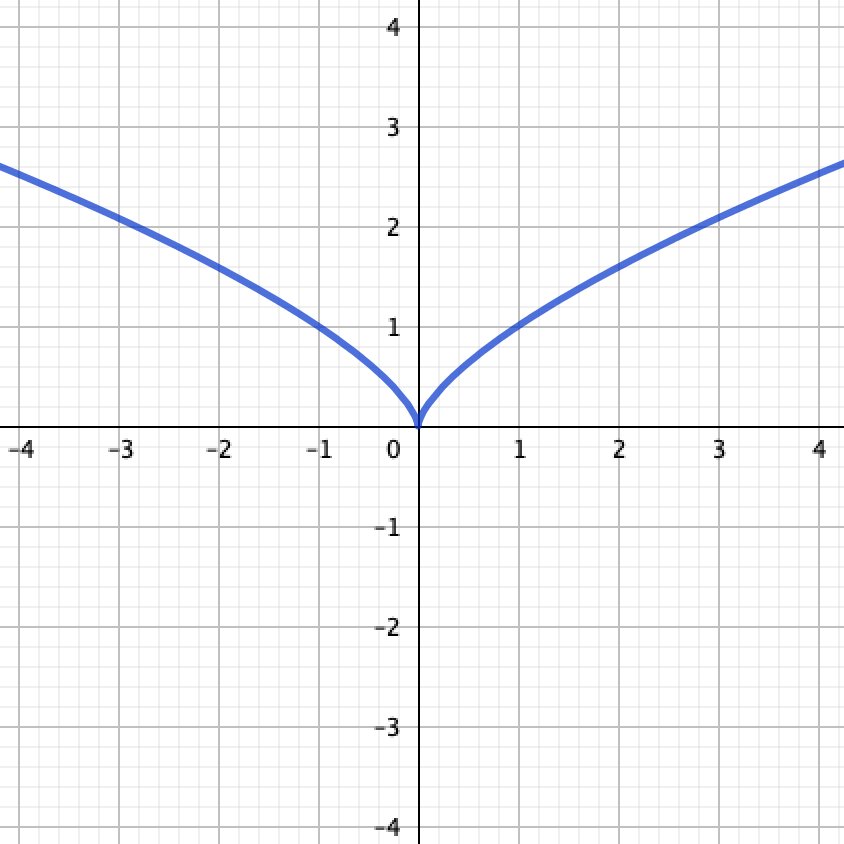
\includegraphics[scale=.5]{curve1}
\end{center}

Note the corner at $(0,0)$; we will see later that this has something to do with our unexpected derivation in the example above.
\end{ex}



\begin{ex} This business about maps of varieties going the wrong way is a bit disorienting. Let's try a couple of examples of this.
\begin{itemize}
\item Given a (radical) ideal $I \subset S=\C[x_1,\dots,x_n]$, the quotient map $S\to S/I$ is given by sending $x_i\mapsto x_i$, so the corresponding map of varieties $V(I)\to \C^n$ is just the inclusion map.
\item Consider $\C[x,y]/(x^2-y^3) \cong \C[t^2,t^3]$ (via $x\mapsto t^3, y\mapsto t^2$) and take the inclusion of rings $\C[t^2,t^3] \subseteq \C[t]$. Under the composition $x\mapsto t^3, y\mapsto t^2$ in $\C[t]$, and corresponding map of varieties goes from $\C\mapsto V(x^2-y^3)$ and sends $b\mapsto(b^3,b^2)$.
\end{itemize}
\end{ex}

One important thing that is \emph{not} included in this correspondence is the usual \emph{Euclidean}\index{Euclidean} topology on $\C^n$ or a subset $X\subseteq \C^n$ with an open basis given by $B_\varepsilon(a) = \{ x \ | \ |x-a|<\varepsilon\}$ with the usual norm $|\cdot |$. We have the \emph{Zariski} topology\index{Zariski} in which the closed sets are subvarieties, but this has no knowledge of what things are close in the Euclidean sense. 

The magic making this all work out so nicely is the Nullstellensatz, which guarantees that maximal ideals of $\C[X]$ all correspond to points of $X$. In general, we just take the (instead of maximal) prime ideals to be our points and work from there.




\begin{center}
\begin{tabular}{c|c}
algebra & ``geometry'' \\ \hline \hline
ring & prime spectrum \\ \hline
 $R$ & $\Spec(R)=\{\fp \ | \ \fp\subset R \ \text{prime ideal}\}$ \\ \hline
prime ideal & point \\ \hline
maximal ideal & closed point \\ \hline
ring homomorphism $R\to S$  & continuous map $Y\to X$ \\
$\phi$ & $\fq \mapsto \phi^{-1}(\fq)$
\end{tabular}
\end{center}

Whereas the correspondence between varieties and reduced f.g. $\C$-algebras was bijective above, the correspondence between rings and their spectra as topological spaces is far from: in particular, every field $K$ has $\Spec(K)$ a singleton. 


\newpage

\sssec{Tangent spaces of varieties}

Let's get to the bottom of this corner business while we're at it. Let's define the \emph{tangent space} of an affine variety $X$ at a point $a$, $T_{a}(X)$. For starters, the tangent space of affine space $\C^n$ at a point $a$ will be the vector space $\C^n$, thought of as centered at $a$. 

\begin{center}
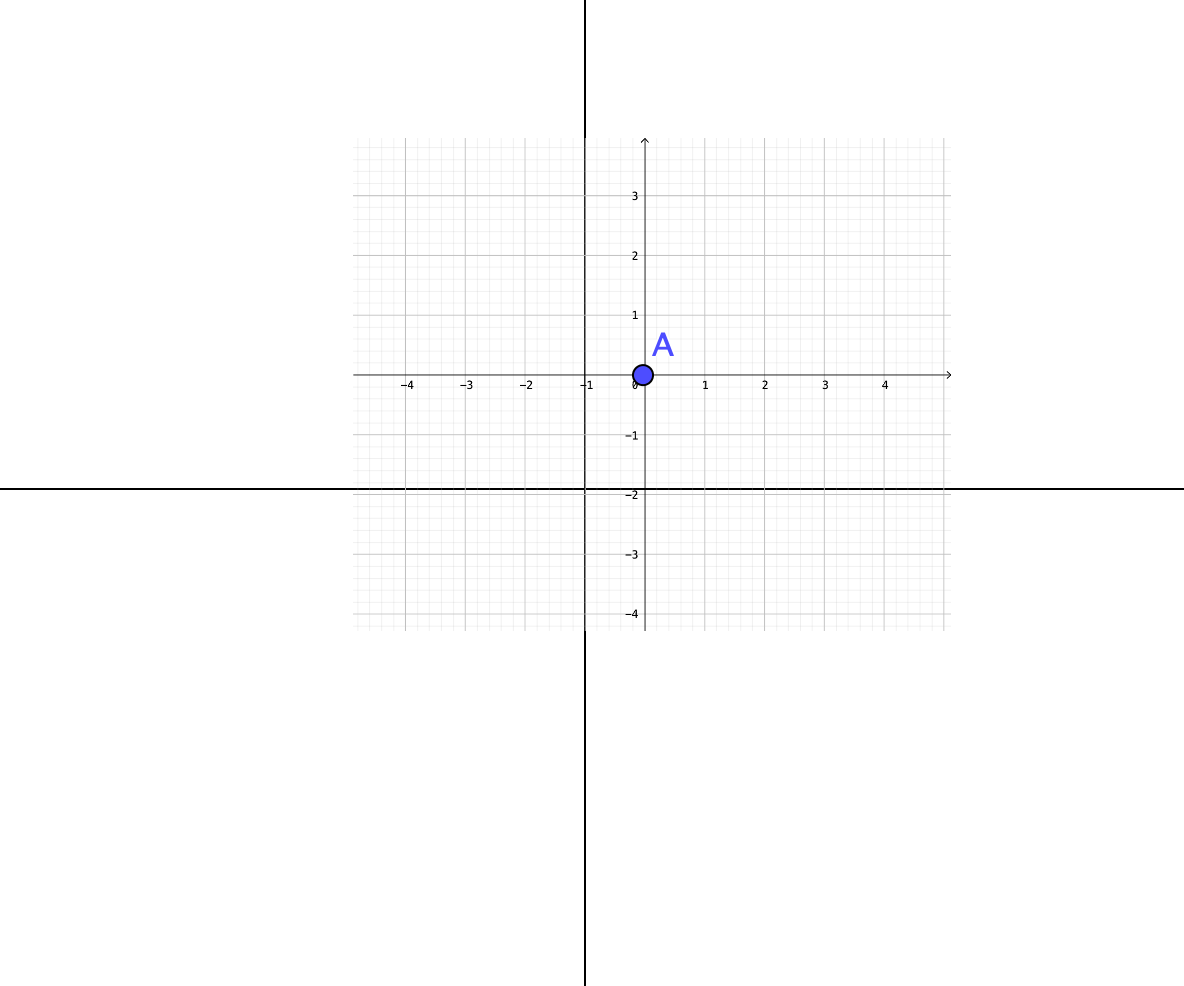
\includegraphics[scale=.4]{tang1}
\end{center}

We can recenter our coordinates there as $\widetilde{x_j}:=x_j-a_j$. Now, given a variety $X=V(f_1,\dots,f_m)$, for each $f_i$ we look at its \emph{linear part}\index{linear part} near $a$: we can take its Taylor expansion at $a$
\[ f_i = f_i(a) + \sum_j \frac{d}{dx_j}|_{x=a}(f_i) (x_j-a_j) + \mathrm{higher \ order \ terms} \ . \]
Since $a\in X$, $f_i(a)=0$, and we have
\[ f_i = \sum_j \frac{d}{dx_j}|_{x=a}(f_i) \widetilde{x_j} + \mathrm{higher\  order\  terms} \ ,\]
so the linear part of $f$ is given by the linear functional $\nabla(f_i)|_{x=a}\cdot \widetilde{x}$. Then we take $T_{a}(X)$ to be the linear subspace of $T_a(\C^n)$ cut out by the linear equations $\nabla(f_1)|_{x=a} v= \cdots = \nabla(f_m)|_{x=a} v = 0$. In particular, $T_a(\C^n)$ is the kernel of the \emph{Jacobian matrix}\index{Jacobian matrix}
\[ J(f_1,\dots,f_m)|_{x=a} = \begin{bmatrix} \frac{d}{dx_1}|_{x=a} (f_1)& \cdots & \frac{d}{dx_n}|_{x=a} (f_1) \\ 
\vdots & \ddots & \vdots \\
\frac{d}{dx_1}|_{x=a} (f_m)& \cdots & \frac{d}{dx_n}|_{x=a} (f_m) \end{bmatrix},\]
whose rows are the gradient vectors.

\Feb{6}
\begin{ex}
Take the parabola $X=V(y - (x-1)^2 -2)$. To compute the tangent space at $a=(1,2)$, take the gradient at $(1,2)$, which is $\begin{bmatrix} -2(x-1) \\ 0\end{bmatrix} |_{(1,2)} =\begin{bmatrix} 0 \\ 1 \end{bmatrix}$, so the defining equation is $\widetilde{y}=0$.
\end{ex}

\begin{center}
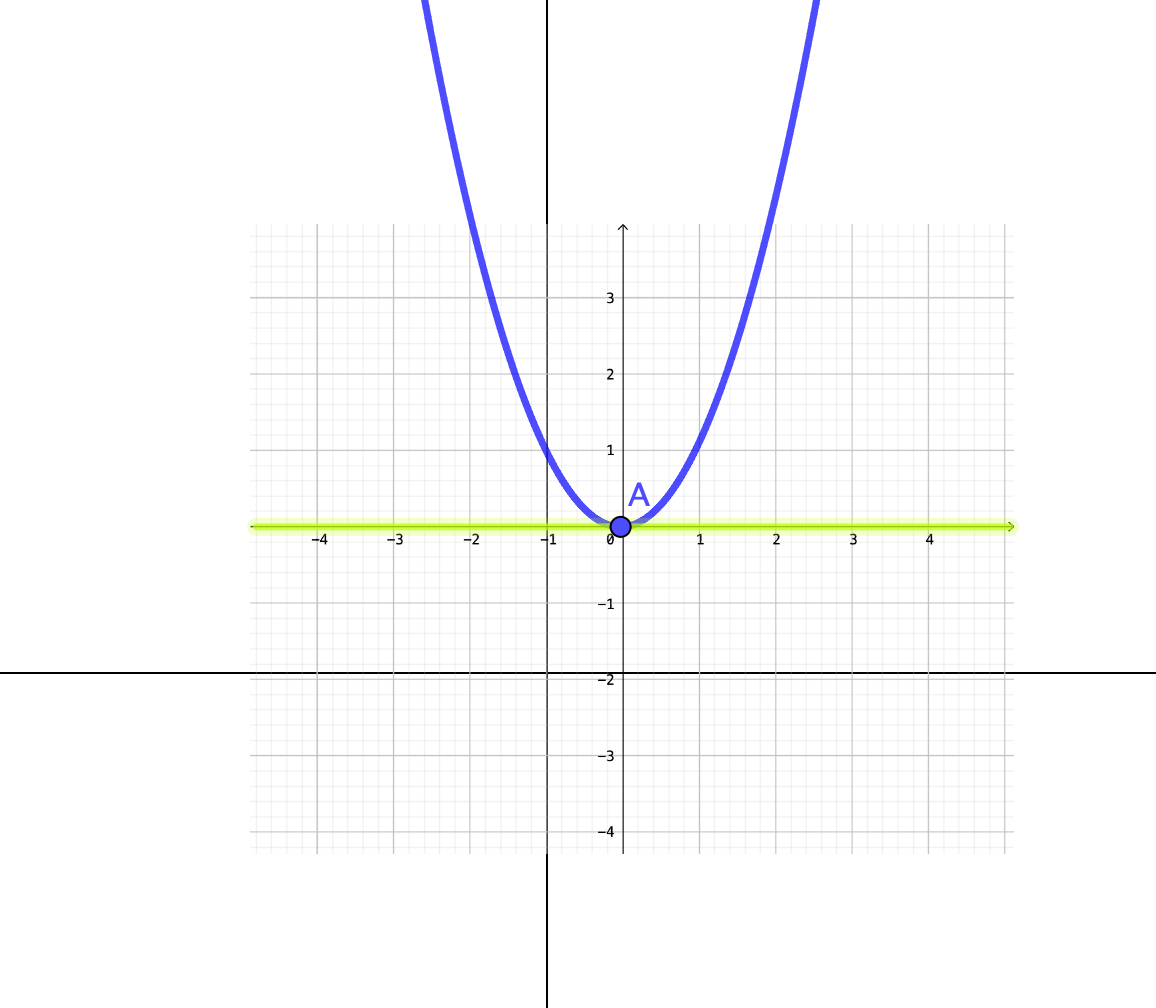
\includegraphics[scale=.4]{tang2}
\end{center}

\begin{ex}
Take the curve $X=V(y^2 - x^3)$. To compute the tangent space at $a=(0,0)$, take the gradient at $(0,0)$, which is $\begin{bmatrix} -3x^2 \\ 2y \end{bmatrix} |_{(0,0)} =\begin{bmatrix} 0 \\ 0  \end{bmatrix}$, so the defining equation is the zero equation. Thus, the tangent space is all of $T_{a}(\C^2)$.
\end{ex}

\begin{center}
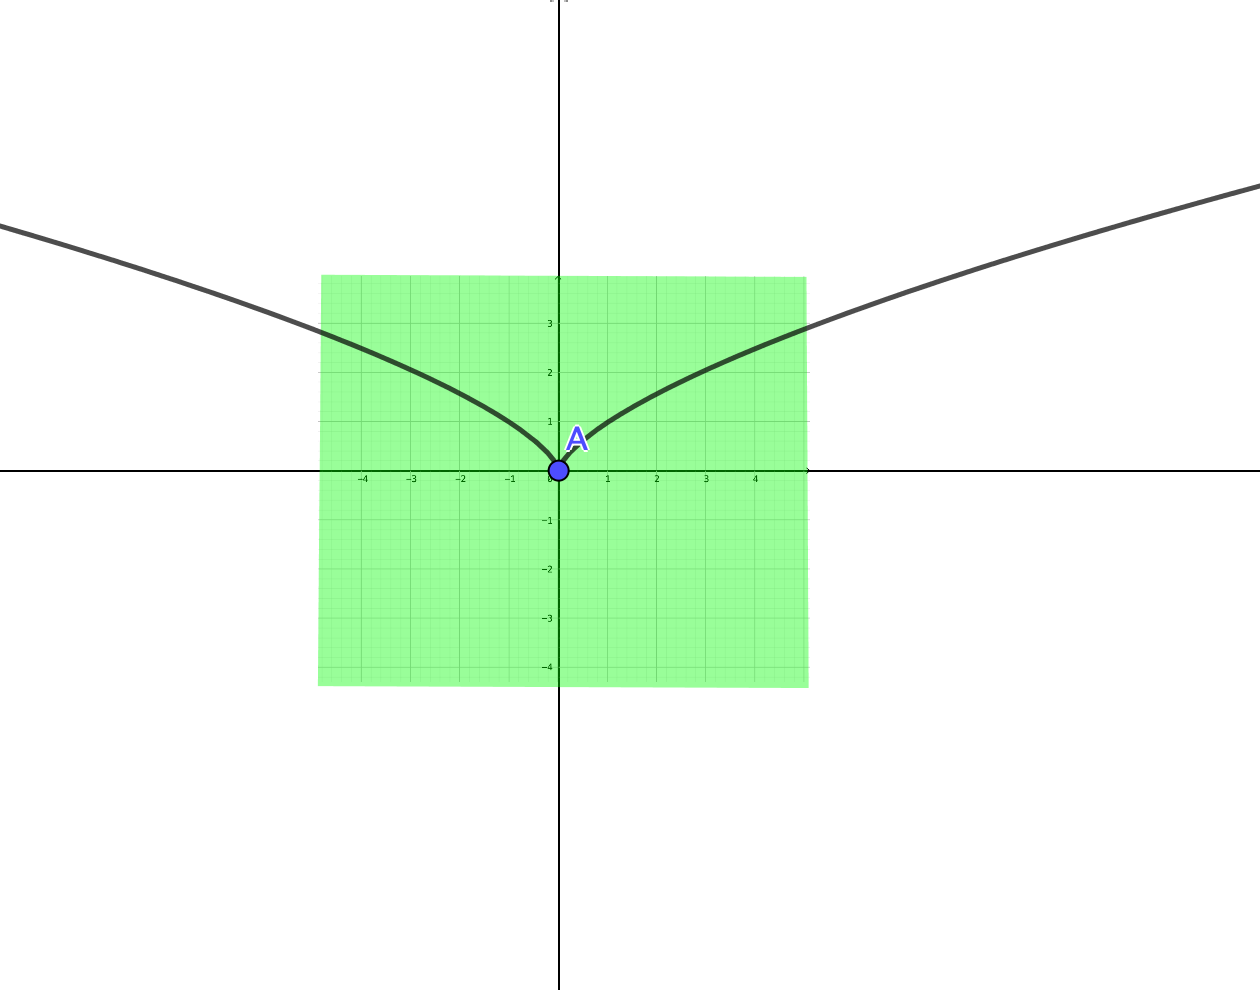
\includegraphics[scale=.4]{tang3}
\end{center}

We want to understand this tangent space in terms of the algebra of the coordinate ring. Here's how.

\begin{prop}
Let $X = V(I)$ be a complex affine variety (with $I$ reduced) and $a\in X$. Let $R=\C[x_1,\dots,x_n]/I$ be the coordinate ring of $X$ and $\fm$ the corresponding maximal ideal. Then there is a $\C$-vector space isomorphism $(\fm/\fm^2)^*\cong T_a(X)$, where $(-)^*$ denotes $\C$-vector space dual.
\end{prop}
\begin{proof} Let $S=\C[x_1,\dots,x_n]$ and $\fn$ be the preimage of $\fm$. Set $\widetilde{x_j} = x_j-a_j$; these are the generators of $\fn$. 
Then  the images of the $\widetilde{x_j}$ form a vector space for $\fn/\fn^2$; we have essentially defined $T_a(\C^n)$ as the $\C$-vector space with coordinates $\widetilde{x_j}$; i.e., the dual space to $\fn/\fn^2$. So $T_a(\C^n)^*\cong \fn/\fn^2$. We will think of $T_a(\C^n)^*= \fn/\fn^2$ each as $1\times n$ row vectors corresponding to the basis $\widetilde{x_j}$ and $T_a(\C^n)$ as $n \times 1$ column vectors.

For an element $f\in \fn$, we can write $f=\nabla(f)|_{x=a}  \widetilde{x}$ in $\fn / \fn^2$, so $\nabla(f)|_{x=a}$ is its row vector.

Then $T_a(X)^*$ corresponds to quotient of the linear functionals on $T_a(\C^n)\to \C$ modulo the ones that vanish on $T_a(X)$. But since $T_a(X)$ is just the set of vectors $v$ such that $\nabla(f_i)|_{x=a} v=0$ for all $i$, a linear functional in $T_a(\C^n)^*$ vanishes on $T_a(X)$ if and only if it is in the (row) span of $\nabla(f_i)|_{x=a}$. Thus, we have \[T_a(X)^* \cong \frac{\fn/\fn^2}{((f_1,\dots,f_m)+\fn^2)/\fn^2} \cong \frac{\fn}{\fn^2+I}.\] Finally, by some basic isomorphism theorems, we can identify $\fm/\fm^2 \cong \fn / (\fn^2+I)$: namely,
\[ \frac{\fm}{\fm^2} \cong \frac{\fn/I}{(\fn^2 + I)/I} \cong \frac{\fn}{\fn^2+I}.\qedhere\]
\end{proof}


\begin{cor} Let $R=\C[X]$ be the coordinate ring of an affine variety and $a\in X$ with associated maximal ideal $\fm$. Then there is an isomorphism $\Der_{R|\C}(R/\fm) \cong T_a(X)$.
\end{cor}

This description of the tangent space of a variety like so is useful; in fact, in many situations, one defines the tangent space to an object by using derivations! Clearly this has some advantages as it naturally arises from $X$ rather than thinking about $X$ inside of $\C^n$ cut out by some equations.



We say that an irreducible affine variety $X$ is \emph{nonsingular} at $a$ if $\dim_\C T_a(X) = \dim X$, and \emph{singular}\index{singular}\index{nonsingular} otherwise (in which case ``$>$'' happens).

\Feb{9}

From the geometric definition of tangent space, we have the following.

\begin{thm}[Jacobian criterion for varieties] Let $X\subseteq \C^n$ be an irreducible affine variety of dimension $d=n-h$. Then
\[ \{a\in X \ | \ X \ \text{is singular at} \ a\} \]
is equal to the vanishing locus of the $h\times h$-minors of $J(f_1,\dots,f_m)$ in $X$.
\end{thm}
\begin{proof}
We have that $T_a(X)=\ker(J(f_1,\dots,f_m)|_{x=a})$, so $\dim(T_a(X)) = n - \mathrm{rank}(J(f_1,\dots,f_m)|_{x=a})$, and so $X$ is singular at $a$ if and only if the rank of $J(f_1,\dots,f_m)|_{x=a}$ is less than $h$. This is equivalent to the all of the $h\times h$ minors of the matrix $J(f_1,\dots,f_m)|_{x=a}$ vanishing. This happens at a point $a$ if and only if each $h\times h$ minor of $J(f_1,\dots,f_m)$ evaluated at $a$ is zero; i.e., $a\in X$ is in the vanishing locus of each $h\times h$ minor.
\end{proof}

\begin{ex} Consider $X=V(x^3-y^2,z-xy)$. The Jacobian matrix is
\[ \begin{bmatrix} 3x^2 & -2y & 0 \\ -y & -x & 1 \end{bmatrix}.\]
Since $X$ has dimension $1$ in $3$ space, we consider the $2\times 2$-minors
\[ -3x^3 - 2y^2, 3x^2, -2y\]
so $x=0, y=0$, and using $z=xy$, $z=0$, and this is the unique singular point on the curve.
\end{ex}


Motivated by the geometric case, for a local ring $(R,\fm,k)$ we define $\fm/\fm^2$ to be the \emph{cotangent space}\index{cotangent space} and $\Hom_k(\fm/\fm^2,k)$ to be the \emph{tangent space}\index{tangent space} of $R$. We recall that a local ring $(R,\fm,k)$ is \emph{regular}\index{regular ring} $\dim(R) = \dim_k(\fm/\fm^2)$.

\begin{ex}
If $R=\C[x_1,\dots,x_n]/I$ is a reduced finitely generated $\C$-algebra, and $\fm$ is a maximal ideal, then $R_{\fm}$ is regular if and only if the variety $X=V(I)$ is nonsingular at $a=V(\fm)$. 
\end{ex}

\begin{ex}
Let $R=\Z_{(2)}$. This is a local ring with maximal ideal $(2)$. The dimension of $R$ is the height of $(2)$ in $\Z$, which is one, and the maximal ideal is generated by one element, so $R$ is regular.
\end{ex}

\begin{ex}
Let $R=\Z[\sqrt{5}]_{(2,1+\sqrt{5})}$. Note that $2,1+\sqrt{5}$ generates a maximal ideal in $\Z[\sqrt{5}]$. The ring $\Z[\sqrt{5}]$ has dimension one, since it is integral over $\Z$, and we see that $R$ has dimension one as well. One can check that the maximal ideal $(2,1+\sqrt{5})$ cannot be generated by one element; equivalently that these elements are $\Z/2\Z$-linearly independent modulo the square of this ideal. Thus, $R$ is not regular.
\end{ex}

{\color{blue}
\begin{rem} It is often handy to use the following fact:

\

Let $R$ be a ring and $\fm$ be a maximal ideal. Let $M$ be an $R$-module such that for every $x\in M$, there is some $n$ such that $\fm^n x=0$. Then the localization map $M\to M_\fm$ is an isomorphism.

\ 

To see it, first note that for any $v\notin \fm$ and and $n\in \N$, there is some $w\notin \fm$ with $vw-1\in \fm^n$. Indeed, since the image of $v$ in $R/\fm$, $v+\fm$, is a unit, there is some $u+ \fm\in R/\fm$ that is its inverse, so $vu+ \fm = 1+\fm$. For an arbitrary representative $u$, we have $vu=1-a$ for some $a\in \fm$. Take $w=u(1+a+a^2+\cdots+a^{n-1})$. Then \[vw=vu(1+a+a^2+\cdots+a^{n-1})=(1-a)(1+a+a^2+\cdots+a^{n-1})=1-a^{n},\]
with $a^n\in \fm^n$.

\

Now, to show that the localization map is injective, we need to check that for any $x\neq 0$, $\frak{x}{1}$ is nonzero as well, so $vx\neq 0$ for any $v\notin \fm$. Take $n$ such that $\fm^n x=0$, and $w\notin\fm$ with $vw-1\in \fm^n$. In particular, $(vw-1)x-0$ so $x=vwx$. Then $0\neq x = vwx$ so $vw\neq 0$.
To show that the localization map is surjective, we show that for any $x\in M$ and $v\notin \fm$, there is some $y\in M$ with $\frac{x}{v} =\frac{y}{1}$. With $n$ and $w$ as above, take $y=wx$: since $vwx=x$, the equality holds.
\end{rem}
}


\ssec{Localization}
 We include one more property of derivations.
 
 \begin{prop} Let $R$ be an $A$-algebra. Let $W \subseteq R$ be a multiplicative set and $V=W\cap A$. For any $W^{-1}R$ module $M$, any $A$-linear derivation $\partial:R\to M$ extends uniquely to an $A$-linear derivation $W^{-1}R \to M$ given by the rule
 \[\widetilde{\partial}\left(\frac{r}{w}\right) = \frac{w \partial(r) - r\partial(w)}{w^2},\]
 and this extension is $V^{-1}A$-linear. Conversely, any $A$-linear derivation from $W^{-1}R \to M$ is of this form.
 
 That is, there are isomorphisms
 \[ \Der_{R|A}(M) \to  \Der_{W^{-1}R|A}(M) \to  \Der_{W^{-1}R|V^{-1}A}(M).\]
 \end{prop}
 \begin{proof}
 We omit the verification that the rule for the map $W^{-1}R \to M$ is well-defined, that this is $V^{-1}A$-linear, and satisfies the product rule. 
 
 If $\alpha:W^{-1}R \to M$ is an $A$-linear derivation, by restriction through the localization map, we get a derivation $\partial:R\to M$ with $\widetilde{\partial} \circ i = \partial$. We claim that $\alpha=\widetilde{\partial}$. Indeed, \[ \partial(r) = \alpha(r) = \alpha(\frac{r}{w} w) = w \alpha(\frac{r}{w}) + \frac{r}{w} \alpha(w) =  w \alpha(\frac{r}{w}) + \frac{r}{w} \partial(w), \]
 so \[\alpha (\frac{r}{w}) = \frac{ \partial(r)-\frac{r}{w} \partial(w) }{w} = \widetilde{\partial}(\frac{r}{w}).\]
 \end{proof}


\Feb{14}

\ssec{Left-exact sequences}

We now encode many of the key properties of derivations in some left-exact sequences. Recall that a sequence of maps of $R$-modules is  a \emph{left exact sequence}\index{left exact sequence} is an exact sequence of $R$-module maps of the form
\[ 0\to L \xra{\alpha} M \xra{\beta} N.\]
That is, $\alpha$ and $\beta$ are $R$-module homomorphisms such that
with $\alpha$  is injective and $\ker(\beta)=\im(\alpha)$.

\begin{prop} Let $R$ be an $A$-algebra and
\[ 0\to L \xra{\alpha} M \xra{\beta} N\]
be a left exact sequence of $R$-modules. Then
\[ 0\to \Der_{R|A}(L) \xra{\alpha_*} \Der_{R|A}(M) \xra{\beta_*} \Der_{R|A}(N)\]
is a left exact sequence, where $\alpha_*(\partial) = \alpha\circ \partial$ and likewise with $\beta_*$.
\end{prop}
\begin{proof} First we observe that $\alpha_*$ is $R$-linear, since $\alpha_*(\partial+\partial') = \alpha_*\partial + \alpha_*\partial'$ and $\alpha_*(r\partial) = r\alpha_*\partial$. 

Since $\alpha$ is injective, if $\partial\neq 0$, then $\alpha_*\partial\neq 0$. If $\beta_*(\partial)=0$, then $\beta \partial (r)=0$ for all $r\in R$, so $\partial(r)\in \ker(\beta)=\im(\alpha)$ for all $r\in R$, and since $\alpha$ is injective, there is an $R$-linear map $\alpha^{-1}:\im(\alpha) \to L$; then $\partial = \alpha_*(\alpha^{-1} \circ \partial) \in \im(\alpha_*)$.
\end{proof}

\begin{prop} Let $A\to R \xra{\phi} S$ be ring homomorphisms, and $M$ be an $S$-module. Then there is a left exact sequence
\[ 0 \to \Der_{S|R}(M) \xra{\inc} \Der_{S|A}(M) \xra{\phi^*} \Der_{R|A}(M)\]
where $\inc$ is the inclusion map and $\phi^*$ is precomposition with $\phi$.
\end{prop}
\begin{proof}
We start by noting that $\Der_{S|R}(M)$ naturally includes in $\Der_{S|A}(M)$, since any $R$-linear map is automatically linear over the image of $A$. 

If $\partial = \inc(\theta)$, then $\phi^*(\partial) = \partial \circ\phi$ is an $R$-linear derivation on $R$, which must be zero. Conversely, if $\phi^*(\partial) =  \partial \circ\phi$ is zero, then $\phi(R)$ is in the kernel of $\partial$, so $\partial$ is $R$-linear, and hence i the image of $\inc$.
\end{proof}

\begin{prop} Let $A\to R  \xra{\pi} R/I$ be ring homomorphisms, and $M$ be an $R/I$-module. Then there is a left exact sequence
\[ 0 \to \Der_{R/I|A}(M) \xra{\pi^*} \Der_{R|A}(M) \xra{\res} \Hom_{\red{R}}(I/I^2,M). \]
\end{prop}
\begin{proof}
First, we have $\pi^*$ is injective, since if $\partial([r])=0$, then $\pi^*(\partial)(r) = \partial \pi(r) = \partial([r])\neq 0$. 

If $\partial=\pi^*(\theta)$, then $\res( \partial) ([a]) =\theta \circ \pi([a]) = \theta (0)$ for $[a]\in I/I^2$, so $\res\circ\pi^*=0$. Conversely, if $\res(\partial)=0$, then $\partial(a)=0$ for all $a\in I$, so $\partial$ yields a well-defined derivation from $R/I\to M$; i.e., is in the image of~$\pi^*$.
\end{proof}

\begin{prop} Let $A\to R  \xra{\pi} R/I$ be ring homomorphisms, and suppose that there is an $A$-algebra homomorphism $\tau:R/I \to R/I^2$ such that $\tau\pi: R\to R/I^2$ is just the quotient map. Then the sequence
\[ 0 \to \Der_{R/I|A}(M) \xra{\pi^*} \Der_{R|A}(M) \xra{\res} \Hom_{\red{R}}(I/I^2,M) \to 0 \]
is exact.
\end{prop}
\begin{proof}
Follows from the previous, plus proposition on surjectivity of res.
\end{proof}


\sec{Kahler differentials}

\ssec{Restriction and extension of scalars}

\sssec{Hom}


\begin{defn} Let $L,M,N$ be $R$-modules.
	\begin{itemize}
		\item The \emph{module of homomorphisms}\index{module of homomorphisms}\index{$\Hom_R(M,N)$} from $M$ to $N$ is 
		\[ \Hom_R(M,N) := \{ \phi:M \to N \ | \ \phi\text{ is $R$-linear}\}.\]
		The $R$-module structure is given by the rule $r \cdot \phi$ is the homomorphism $m \mapsto r \phi(m) = \phi(rm)$.
		\item If $\alpha: M\to N$ is a module homomorphism, we define a map $\Hom_R(L,\alpha)$ or $\alpha_*$\index{$\Hom_R(L,\alpha)$}\index{$\alpha_*$} from $\Hom_R(L,M)\to \Hom_R(L,N)$ by the rule
		\[ \alpha_*{(\phi)} =  \alpha \circ \phi ;\]
		i.e.,
		\[ \alpha_* : \qquad (\ L\xrightarrow{\phi} M \ ) \ \ \mapsto \ \ (\ L \xrightarrow{\alpha }M\xrightarrow{\phi} N \ ).   \]
			\item If $\alpha: M\to N$ is a module homomorphism, we define a map $\Hom_R(\alpha,L)$ or $\alpha^*$\index{$\Hom_R(\alpha,L)$}\index{$\alpha^*$} from $\Hom_R(N,L)\to \Hom_R(M,L)$ by the rule
		\[ \alpha^*{(\phi)} = \phi \circ \alpha;\]
		i.e.,
		\[ \alpha^* : \qquad (\ N\xrightarrow{\phi} L \ ) \ \ \mapsto \ \ (\ M \xrightarrow{\alpha }N\xrightarrow{\phi} L \ ).   \]
	\end{itemize}
\end{defn}

Thus, given a fixed $R$-module $L$, $F(-):=\Hom_R(L,-)$ is a rule that assigns to any $R$-module $M$ another $R$-module $F(M)$, and to any homomorphism $M \xrightarrow{\phi} N$ a homomorphism $F(M) \xrightarrow{F(\phi)} F(N)$. This plus the fact that $F$ takes the identity map to the identity map and compositions to compositions makes $F$ a \emph{covariant functor}\index{covariant functor} from $R$-modules to $R$-modules.

Similarly, given a fixed $R$-module $L$, $G(-):= \Hom_R(-,L)$ is rule that assigns to any $R$-module $M$ another $R$-module $G(M)$, and to any homomorphism $G(M) \xrightarrow{\phi} G(N)$ a homomorphism $G(N) \xrightarrow{G(\phi)} G(M)$. This plus the fact that $F$ takes the identity map to the identity map and compositions to compositions makes $G$ a \emph{contravariant functor}\index{contravariant functor} from $R$-modules to $R$-modules. The covariant vs.~contravariant bit refers to whether the directions of maps have changed.

Given maps $L \xrightarrow{\alpha} L'$ and $M \xrightarrow{\beta} M'$, we likewise get a map $\Hom_R(L',M) \xrightarrow{\Hom_R(\alpha,\beta)} \Hom_R(L,M')$, by combining the constructions above.

\begin{ex}
$\Hom_R(R,M)\cong M$ by $\phi\mapsto \phi(1)$, and under this isomorphism, $M \xrightarrow{\alpha} N$ corresponds to $1 \mapsto m \rightsquigarrow 1 \mapsto \alpha(m)$ under this isomorphism.

If $I$ is an ideal, $\Hom_R(R/I,M)\cong \ann_M(I)$ by the same map: the image of $1$ in $R/I$ must map to something killed by $I$, and there is a unique $R$-linear map that does this. The same recipe for maps as above holds. Thus, we can identify $\Hom_R(R/I,-)$ with the functor that sends modules $M$ to $\ann_M(I)$, and sends maps to their restrictions to these submodules.
\end{ex}

We recall that a sequence of maps of $R$-modules is \emph{split-exact} if it is of the form
\[ 0 \to L \xra{\alpha} M \xra{\beta} N \to 0\]
with $\alpha$ injective, $\beta$ surjective, $\ker(\beta)=\im(\alpha)$ and $\alpha$ has a left inverse (i.e., there is a map $\rho$ such that $\rho \alpha$ is the identity on $L$). It is equivalent if we replace the last condition with $\beta$ has a right inverse (i.e., there is a map $\iota$ such that $\beta \iota$ is the identity on $N$.

\begin{thm}
	\begin{enumerate}
		 \item	A sequence of maps \[ 0 \to L \xrightarrow{\alpha} M \xrightarrow{\beta} N\]
		is exact if and only if, for all $R$-modules $X$, the sequence
		\[ 0 \to \Hom_R(X,L) \xrightarrow{\alpha_*} \Hom_R(X,M) \xrightarrow{\beta_*} \Hom_R(X,N)  \]
		is exact.
		\item A sequence of maps \[ 0 \to L \xra{\alpha} M \xra{\beta} N \to 0\] is split-exact if and only if, for all $R$-modules $X$, the sequence
		\[ 0 \to \Hom_R(X,L) \xrightarrow{\alpha_*} \Hom_R(X,M) \xrightarrow{\beta_*} \Hom_R(X,N) \to 0 \]
		is exact.

\item	A sequence of maps \[ L \xrightarrow{\alpha} M \xrightarrow{\beta} N \to 0 \]
is right-exact if and only if, for all $R$-modules $X$, the sequence
\[ 0 \to \Hom_R(N,X) \xrightarrow{\beta^*} \Hom_R(M,X) \xrightarrow{\alpha^*} \Hom_R(L,X)  \]
is left-exact.
\item A sequence of maps \[ 0 \to L \xra{\alpha} M \xra{\beta} N \to 0\] is split-exact if and only if, for all $R$-modules $X$, the sequence
\[ 0 \to \Hom_R(N,X) \xrightarrow{\beta^*} \Hom_R(M,X) \xrightarrow{\alpha^*} \Hom_R(L,X) \to 0 \]
is exact.
\end{enumerate}
\end{thm}
\begin{proof}
\begin{enumerate}
\item
 Let $0 \to L \xrightarrow{\alpha} M \xrightarrow{\beta} N$ be exact, and $X$ be an $R$-module. 
 \begin{itemize}
 \item $\alpha_*$ is injective: if $X \xrightarrow{\phi} L$ is nonzero, $X \xrightarrow{\phi} L \xrightarrow{\alpha} M$ is as well, since a nonzero element in the image of $\phi$ goes to something nonzero in the composition.
\item $\ker(\beta_*)=\im(\alpha_*)$: $X \xrightarrow{\phi} M \xrightarrow{\beta} N$ is zero if and only if $\im(\phi) \subseteq \ker(\beta) = \im(\alpha)$, which happens if and only if $\phi$ factors through $L$; i.e., $\phi\in \im(\alpha_*)$.
\end{itemize}

  The other direction of the first part follows from the example above; we can use $X=R$.

\item Let $0 \to L \xrightarrow{\alpha} M \xrightarrow{\beta} N \to 0$ be split-exact, and $X$ be an $R$-module. In particular, $0 \to L \xrightarrow{\alpha} M \xrightarrow{\beta} N$ is a left exact sequence, so 
\[ 0 \to \Hom_R(X,L) \xrightarrow{\alpha_*} \Hom_R(X,M) \xrightarrow{\beta_*} \Hom_R(X,N)  \]
		is exact. We just need to see that $\Hom_R(X,M) \xrightarrow{\beta_*} \Hom_R(X,N) $ is surjective. Let $\iota$ be such that $\beta\iota$ is the identity on $N$. Then $\beta_*\iota_*$ is the identity on $\Hom_R(X,M)$, so $\beta_*$ must be surjective.
		
		For the converse, take $X=N$. Then the identity map in $\Hom_R(N,N)$ is in the image of $\beta_*$, so there is a map $\rho\in \Hom_R(M,N)$ such that $\beta \rho =\beta_*(\rho)$ is the identity on $N$, as required.
 
\item  Let $L \xrightarrow{\alpha} M \xrightarrow{\beta} N \to 0$ be a right-exact sequence, and $X$ be an $R$-module.
  \begin{itemize}
\item   $\beta^*$ is injective: if $N \xrightarrow{\phi} X$ is nonzero, pick $n\in N$ not in the kernel, and $m\in M$ that maps to $n$. Then, the image of $m$ under $ M \xrightarrow{\beta} N \xrightarrow{\phi} X$ is nonzero.
 \item $\ker(\alpha^*)=\im(\beta_*)$: $ L \xrightarrow{\alpha} M \xrightarrow{\phi} X$ is zero if and only if $\im(\alpha)\subseteq \ker(\phi)$, which happens if and only if $\phi$ descends to a map of the form $N \cong M/\im(\alpha) \to X$; i.e., $\phi \in \im(\alpha^*)$.
\end{itemize}
 Let $L \xrightarrow{\alpha} M \xrightarrow{\beta} N \to 0$ be a sequence of maps, and suppose that it is exact after applying $\Hom_R(-,X)$ for all $X$.
  
   \begin{itemize}\item $\beta$ is surjective: if not, let $X=N/\im(\beta)$. There is a nonzero projection map $N \xrightarrow{\phi} X$, but $M \xrightarrow{\beta} N \xrightarrow{\phi} X$ is zero, contradicting injectivity of $\beta^*$.
\item  $\ker(\beta)\supseteq \im(\alpha)$: Take $X=N$, and $N\xrightarrow{\mathrm{id}} X$. Since $\ker(\alpha^*)\supseteq \im(\beta^*)$, $L \xrightarrow{\alpha} M \xrightarrow{\beta} N\xrightarrow{\mathrm{id}} X = L \xrightarrow{\alpha} M \xrightarrow{\beta} N$ is zero.
 \item $\ker(\beta)\subseteq \im(\alpha)$: Take $X=M/\im(\alpha)$, and $M \xrightarrow{\phi} X$ the projection map. Since $L \xrightarrow{\alpha} M \xrightarrow{\phi} X$ is zero, $\phi$ is in the image of $\beta^*$, so it factors through $\beta$. This is equivalent to the stated containment.
 \end{itemize}
 
 \item Similar to (2). \qedhere
 
 \end{enumerate}
 
\end{proof}

In short, $\Hom_R(X,-)$ is kernel-preserving, and $\Hom_R(-,X)$ turns cokernels into kernels.

Given a ring homomorphism $\phi:R\to S$, we can use $\phi$ to turn $S$-modules and $S$-algebras into $R$-modules and $R$-algebras with \emph{restriction of scalars} and vice versa with \emph{extension of scalars}.

\sssec{Restriction of scalars}

Given $\phi:R\to S$ and an $S$-module $N$, we get an $R$-module $\phi_*(N)$\index{$\phi_*$} by \emph{restriction of scalars}\index{restriction of scalars} by keeping the same set and same addition, so $\phi_*(N)=N$ as additive groups, and the $R$-module action $r\cdot  n := \phi(r) \cdot n$, where the left-hand side is the action in $\phi_*(N)$ and the right hand side is the original $S$-action. When $\phi: R\to S$ is just an inclusion map $R\subseteq S$, this restriction of scalars is literally just restricting which scalars we consider in the module action. 

For example, consider $R=\C \subseteq S=\C[x]$ and $N=\C[x]/(x^3)$. $N$ is a cyclic $S$-module killed by some stuff, but we can also ``forget about the action of $x$'' and consider $N$ as a $\C$-vectorspace; as such it is just a free $3$-generated $R$-module.

Given a homomorphism of $S$-modules $\alpha:N \to N'$, we can call $\phi_*(\alpha)$ the same map from $\phi_*(N)\to \phi*(N)$, which is a homomorphism of $R$-modules.

We can think of this restriction of scalars $\phi_*$ as the ``demotion''\index{demotion} functor, when demotes modules from a ``bigger'' (target of $\phi$) ring to a ``smaller'' (source of $\phi$) ring.

In the same way, we can demote $S$-algebras to $R$-algebras: if $T$ is an $S$-algebra with structure map $\psi:S\to T$ take $\phi_*(T)$ to be the same ring $T$ with structure map $\psi\circ \phi:R\to T$.

To promote a module or an algebra, we have to do something a bit more interesting. For example, consider $R= \C \subseteq S=\C[x]$ and $M=\C^3$, a free $R$-module of rank $3$. There is no ``obvious'' or ``natural'' $R$-module structure on $M$, so we'll end up changing our underlying set. The ``right'' way of going about this is by using tensor products, but we'll take a barehanded approach using presentations, and everyone is encouraged to reconcile the two approaches now if they know tensors and, if not, later when they do.

\sssec{Presentations of modules}

Let $M$ be an $R$-module.

Given a generating set $\{m_\lambda\}_{\lambda\in \Lambda}$ for $M$, there is a surjection from a free module onto $M$:
\[\xymatrix@R=0pc{  \{m_\lambda\}_{\lambda\in \Lambda}  & \rightsquigarrow & R^{\oplus \Lambda} \to M \to 0 \\  \text{generating set} & &  e_\lambda \mapsto m_\lambda \ \ \ }\]
and conversely any such surjection yields a generating set (consisting of the images of the basis vectors).

The kernel of this map is a submodule of $R^{\oplus \Lambda}$ which are the relations on these generators. We can take a subset $\{v_\gamma\}_{\gamma\in \Gamma}$ that generates the module of relations (a set of \emph{defining relations}) and map a free module onto them:
\[\xymatrix@R=0pc@C=.5pc{  \{m_\lambda\}_{\lambda\in \Lambda}  & + & \{v_\gamma\}_{\gamma\in \Gamma} &  \rightsquigarrow & R^{\oplus \Gamma} \longrightarrow R^{\oplus \Lambda} \longrightarrow M \to 0 \\  \text{generating set} & & \text{defining relations} &  & e'_\gamma \mapsto v_\gamma \ \ e_\lambda \mapsto m_\lambda \ \ \ \ }\]
Conversely, any such right exact sequence is a recipe for a set of generators and defining relations on $M$. The map between free modules is given by multiplication by a (possibly infinite) matrix $A$ whose $\gamma$ column consists of the $\lambda$-coordinates of $v_\gamma$; concretely, each column is a relation on the $m_\lambda$'s. When $\Lambda$ and $\Gamma$ are finite, we'll just write something like
\[ R^m \xrightarrow{A} R^n \to M \to 0\]
and $A$ will be an actual $n\times m$ matrix, standing for the map of  multiplication (on the left) by $A$. We will call this (either in the finite or infinite case) a \emph{presentation matrix}\index{presentation matrix} for $M$. 

Given a presentation matrix, we can recover $M$ up to isomorphism as $M\cong R^n/\im(A)$ (i.e., the \emph{cokernel}\index{cokernel} of the map $A$) coming from the first isomorphism theorem, since the map from $R^n\to M$ is surjective with kernel $\im(A)$. The rows of the presentation matrix correspond to generators, and the columns correspond to relations.






\sssec{Extension of scalars for modules}
We're now ready to describe \emph{extension of scalars}\index{extension of scalars}, or \emph{promotion}\index{promotion} of a module along a ring homomorphism. Let $\phi:R\to S$ be a ring homomorphism and $M$ be an $R$-module. We define the extension of scalars of $M$, denoted $\phi^*(M)$ or $S\otimes_R M$\index{$\phi^*(M)$}\index{$S\otimes_R M$} as follows. Take a presentation of $M$:
\[ R^m \xra{A} R^n \to M \to 0;\]
then $\phi^*(M)$ is the $S$-module with the same presentation
\[ S^m \xra{\phi(A)} S^n \to \phi^*(M) \to 0.\]

\Feb{16}

It's not clear that what we did does not depend on the choice of presentation. However, we will show that the $\phi^*(M)$ satisfies an important universal property and use that to show it is well-defined.

First we note that there is an $R$-module homomorphism from $\eta_M: M \to \phi^*(M)$ (or more properly, to $\phi_*\phi^*(M)$). Given $r\in R$ write $m= \sum_i r_i [e_i]$, where the $e_i$'s are the standard basis in $R^n$. For convenience, set $\mathbf{e}$ to be the row vector with entries $e_1,\dots,e_n$ and $\mathbf{r}$ be the column vector of $r_1,\dots, r_n$ so $m= \mathbf{e}\mathbf{r}$. We map $m$ to $\mathbf{e} \phi(\mathbf{r}) = \sum_i \phi(r_i) [e_i]$. If $m$ also equals $\sum_i r'_i [e_i] = \mathbf{e}\mathbf{r'}$, then $\mathbf{e}(\mathbf{r}-\mathbf{r'})= 0$ so $\mathbf{r}-\mathbf{r'} = A\mathbf{v}$ for some $\mathbf{v}$, and hence \[ \mathbf{e} \phi(\mathbf{r}) - \mathbf{e} \phi(\mathbf{r'}) = \mathbf{e} \phi(\mathbf{r}-\mathbf{r'}) = \mathbf{e} \phi(A\mathbf{v}) = \mathbf{e} \phi(A) \mathbf{v},\]
so this is zero in $\phi^*(M)$. It is then clear to see that this is $R$-linear. 

\begin{prop}
Let $\phi:R\to S$ be a ring homomorphism. Let $M$ be an $R$-module, $N$ be an $S$-module, and $\alpha:M \to \phi_*(N)$ be an $R$-module homomorphism. Then there exists a unique $S$-module homomorphism $\beta: \phi_*(M) \to N$ that makes the diagram commute:
\[ \xymatrix{  M \ar[r]^-{\eta_M} \ar[dr]_-{\alpha} & \phi^*(M) \ar@{-->}[d]^-{\beta} \\ & N}.\]
\end{prop}
\begin{proof} We will abuse notation and drop the $\phi$ to identify elements in $R$ with their images in $S$.

Let $\alpha([e_i]) = n_i$ and write $\bs{n}$ for the row vector $[n_1,\dots,n_t]$. We define $\beta( \sum_i s_i [e'_i] ) = \sum_i s_i n_i$, or $\beta(\mathbf{e}\mathbf{s}) = \mathbf{n}\mathbf{s}$ for short. To see that this is well-defined, suppose that $\sum_i s_i [e'_i] = \sum_i s'_i [e'_i]$, and write $\bs{s}$ and $\bs{s'}$ for the column vectors of $s_i$ and $s'_i$. We need to show that $\bs{n}\bs{s}=\bs{n}\bs{s'}$. By construction of $\phi^*(M)$, we have that $\bs{s}-\bs{s'} = A \bs{v}$ for some vector $\bs{v}$ with entries in $S$. Since $\alpha$ is well-defined, we must have that for any columns of $A$, the corresponding combination of basis vectors maps to zero, so the corresponding combination of the $n$'s is zero; i.e., $\bs{n} A=0$. But then $\bs{n} A \bs{v} = \bs{n} (\bs{s}-\bs{s'})$, and this shows the claim. Checking $S$-linearity is straightforward from the construction.
 For uniqueness, $\phi^*(M)$ is generated by $[e_i]$, and $n_i = \alpha([e_i])= \beta \eta_M([e_i])=\beta([e'_i])$, so the generators must go to the same place, and hence there can only be one map.
\end{proof}

In other words, the proposition says that for any $R$-module $M$ and $S$-module $N$, there is an isomorphism 
\[  \Hom_S(\phi^*M,N) \xra{\eta_M^*} \Hom_R(M,\phi_* N).\]

\begin{cor}
 $\phi:R\to S$ be a ring homomorphism, and $M$ be an $R$-module. Fix two presentations for $M$, and let $(\phi_1^*(M),\eta^M_1)$ and $(\phi^*_2(M), \eta^M_2)$ be the two modules and morphisms constructed above for each presentation. Then $\phi^*_1(M)\cong \phi^*_2(M)$ as $S$-modules. Moreover, there is a unique $S$-module isomorphism $\theta$ for which $\eta^M_2 = \theta \circ \eta^M_1$.
\end{cor}
\begin{proof}
It suffices to show that there is an isomorphism that makes $\eta^M_2 = \theta \circ \eta^M_1$, for the uniqueness will follow from the proposition applied with $\alpha=\eta_2$.
Consider the diagram
\[ \xymatrix{ & \phi^*_1(M) \ar@{-->}[d]\\
M \ar[ur]^{\eta_1} \ar[r]^{\eta_2} \ar[dr]_{\eta_1} & \phi^*_2(M)\ar@{-->}[d] \\
& \phi^*_1(M)}\]
The universal property yields unique $S$-module dotted maps making the triangles commute. The double down composition and the identity map on $\phi^*_1(M)$ are two maps that make the big triangle commute. Applying the uniqueness in the proposition with $\alpha=\eta_1$, we get that the composition is the identity. We can switch the roles of $\phi^*_1$ and $\phi^*_2$ to get that the other composition is the identity. Thus, the induced map is an isomorphism.
\end{proof}

\begin{cor}
Let $\phi:R\to S$ be a ring homomorphism. For any $R$-module homomorphism $\alpha:M\to N$, there is a unique $S$-module homomomorphism $\phi^*\alpha:\phi^*M \to \phi^*N$ such that $\phi^*\alpha \circ \eta_M = \eta_N \circ \alpha$.
\end{cor}
\begin{proof} 
Apply the universal property of $(\phi^*M, \eta_M)$ to $\eta_N \circ \alpha$.
\end{proof}

Tracing the proof of the universal property, we see that $\phi^*\alpha$ can be computed as follows: take presentations for $M$ and $N$, and
lift $\alpha$ to a matrix from the free modules over $M$ and $N$; then use the same matrix for $\phi^*\alpha$.

\begin{lem} Under the isomorphisms $\Hom_S(\phi^*M,N) \xra{\eta_M^*} \Hom_R(M,\phi_* N)$, the map $\Hom_S(\phi^*\alpha,N)$ corresponds to $\Hom_R(\alpha,N)$.
That is, for an $R$-module homomorphism $\alpha:L\to M$ and $S$-module $N$, there is a commutative diagram:
\[\xymatrix@C=5em{
 \Hom_S(\phi^* M, N) \ar[r]^{\Hom_S(\phi^*\alpha,N)} \ar[d]^{\eta_M^*}_{\cong} &  \Hom_S(\phi^* L, N) \ar[d]^{\eta_L^*}_{\cong} \\
 \Hom_R(M,N) \ar[r]^{\Hom_R(\alpha,N)} & \Hom_R(L,N)
}\]
\end{lem}
\begin{proof}
First, by construction of $\phi^*\alpha$, we have a commutative diagram:
\[ \xymatrix{
\phi^*M & \ar[l]_{\phi^* \alpha} \phi^* L \\
M \ar[u]_{\eta_M} & L \ar[l]_{\alpha} \ar[u]_{\eta_L}}\]
Then using this commutativity, given an $S$-linear map $\theta:\phi^*M \to N$, we have that
\[(\eta_L^* \circ \Hom(\phi^*\alpha,N)) (\theta) = \theta \circ \phi^*\alpha \circ \eta_L = \theta \circ \alpha \circ \eta_M = (\Hom(\alpha,N) \circ \eta_M^*)(\theta).\qedhere\]
\end{proof}

\begin{prop} Let $\phi:R\to S$ be a ring homomorphism, and 
\[ L \xra{\alpha} M \xra{\beta} N \to 0\]
be a right exact sequence of $R$-modules. Then the sequence of $S$-modules
\[ \phi^*L \xra{\phi^*\alpha} \phi^*M \xra{\phi^*\beta} \phi^*N \to 0\]
is exact.
\end{prop}
\begin{proof}
Let $X$ be an arbitrary $S$-module. Applying Hom into $X$ to the sequence above, we have a sequence:
\[ 0 \to \Hom_S(\phi^*N,X)  \xra{\Hom(\phi^*\beta,X)} \Hom_S(\phi^*M,X) \xra{\Hom(\phi^*\alpha,X)} \Hom_S(\phi^*L,X).\]
We have isomorphisms
\[ \xymatrix@C=5em{ 
0 \ar[r] \ar@{=}[d]  & \Hom_S(\phi^*N,X)  \ar[r]^{\Hom(\phi^*\beta,X)} \ar@{=}[d] & \Hom_S(\phi^*M,X) \ar[r]^{\Hom(\phi^*\alpha,X)} \ar@{=}[d] & \Hom_S(\phi^*L,X) \ar@{=}[d] \\
0 \ar[r] & \Hom_R(N,X) \ar[r]^{\Hom(\beta,X)} & \Hom_R(M,X) \ar[r]^{\Hom(\alpha,X)} & \Hom_R(L,X) }\]
The last row is exact, by left exactness of Hom (part (3) in the forward implication). But then by left exactness of Hom again, since this is true for all $X$, the sequence we consider is exact.
\end{proof}

In general, exact sequences (or left exact sequences) no longer remain exact. We say that a ring homomorphism $\phi:R\to S$ is \emph{flat}\index{flat} if it has the special property that extension of scalars preserves exact sequences.

\begin{prop} Let $R$ be a ring and $W$ be a multiplicative set. Let $\phi:R\to W^{-1}R$ be the localization map. Then $\phi^*(M)\cong W^{-1}M$ for any $R$-module $M$.
\end{prop}
\begin{proof} Let $\eta:M \to W^{-1}M$ be the localization map. We will show that $(W^{-1}M,\eta)$ satisfies the universal property of $\phi^*M$. If $N$ is any $W^{-1}R$-module, and $\alpha:M\to N$ is a homomorphism, define $\beta:W^{-1}M \to N$ by sending $\beta(\frac{m}{w}) = \frac{\alpha(m)}{w}$. The check that this $\beta$ is well-defined and $W^{-1}R$-linear is straightforward; that it is the unique map making the diagram commute follows from the fact that the image of $M$ generates $W^{-1}M$ as a $W^{-1}R$-module.
\end{proof}



\sssec{Presentations of algebras}
We can play a similar game with algebras. Let $S$ be an $R$-algebra, so there is some $\phi:R\to S$. Given a generating set for $S$ as an algebra, we get a surjection from a polynomial ring:
\[\xymatrix@R=0pc{  \{s_\lambda\}_{\lambda\in \Lambda}  & \rightsquigarrow & R[\{x_\lambda\}_{\lambda\in\Lambda}] \to S  \to 0 \\  \text{algebra generating set} & & \ \ \ \ \ \ x_\lambda \mapsto s_\lambda }\]
The kernel is an ideal $I$, for which we can pick generators $(\{f_\gamma\}_{\gamma\in \Gamma})$ and we get
\[\xymatrix@R=0pc@C=.5pc{  \{s_\lambda\}_{\lambda\in \Lambda}  & + & \{f_\gamma\}_{\gamma\in \Gamma} &  \rightsquigarrow & R[\{x_\lambda\}_{\lambda\in\Lambda}]^{\oplus \Gamma}  \longrightarrow R[\{X_\lambda\}_{\lambda\in\Lambda}] \longrightarrow S \to 0 \\  \text{algebra generating set} & & \text{defining relations} &  & \quad \qquad e'_\gamma \mapsto f_\gamma \qquad \qquad e_\lambda \mapsto s_\lambda }\]
Note that we have \emph{polynomial} relations rather than linear relations now, so we can't use a matrix to describe them anymore. 


Given an $R$-algebra $S$ with an algebra presentation $S\cong R[x_1,\dots,x_n]/(f_1,\dots,f_m)$, we can also ask what $S$ looks like as an $R$-module. As a generating set, we can take the monomials $\{x_1^{a_1}\cdots x_n^{a_n} \ | \ a_i\in \N\}$. The relations are generated as an $R[x_1,\dots,x_n]$-module by $f_1,\dots, f_m$; to find an $R$-module generating set of the relations, we can take $\{ x_1^{a_1}\cdots x_n^{a_n} f_j \ | \ a_i\in \N, j=1,\dots,m\}$ and collect the coefficients of the monomials, and this gives a presentation. That is, if $f_j = \sum_a c_{a,j} x^a$ for some tuples $a$, then $\{\sum_a c_{a,j} x^{a+b} \ | \ b\in \N^n, j=1,\dots,m\}$ is a defining set of relations. 

For example, consider $R=\Z[x]/(2x^2-5)$. Let's find a $\Z$-module presentation of this ring. As a generating set, we have $1,x,x^2,x^3,\dots$; the relations are given by $2x^2-5, 2x^3 -5x, 2x^4-5x^2, \dots$; the presentation matrix is
\[ \begin{bmatrix} 
-5 & 0 & \cdots & & \\
0 & -5 & 0 & \cdots & \\
2 & 0 & -5 & 0 & \cdots \\
0 & 2 & 0 & -5 & \ddots \\
& \ddots & \ddots & \ddots & \ddots \end{bmatrix}\]



\sssec{Base change for algebras}


Let's promote some algebras too. We'll follow the same recipe: take a presentation (as an algebra) and upgrade the base ring. That is, let $\phi:R\to S$ be a ring homomorphism and $T$ be an $R$-algebra. We define the \emph{extension of scalars}\index{extension of scalars} or \emph{base change}\index{base change} of $T$ as follows. Write
\[ R[X_1,\dots,X_n]^{m} \xra{[f_1,\dots,f_m]} R[X_1,\dots,X_n] \to T \to 0;\]
then $\phi^*(T)$ is the $S$-algebra with presentation
\[ S[X_1,\dots,X_n]^{m} \xra{[\phi(f_1),\dots,\phi(f_m)]} S[X_1,\dots,X_n] \to \phi^*(T) \to 0.\]

Note that we are using the same notation as module extension of scalars, though it is not immediately clear these should be related. For starters, in analogy with the module extension of scalars, one has:

\begin{prop} For a ring homomorphism $\phi:R\to S$ and an $R$-algebra $T$, the base change $\phi^*T$ 
admits an $R$-algebra homomorphism $\eta_T: T\to \phi^*T$ that satisfies the universal property that for any $S$-algebra $V$ and $R$-algebra homomorphism $\alpha:R\to V$, there is a unique $S$-algebra homomorphism $\beta: \phi^*T\to V$ that makes the diagram commute:
\[  \xymatrix{  T \ar[r]^-{\eta_T} \ar[dr]_-{\alpha} & \phi^*T \ar@{-->}[d]^-{\beta} \\ & V}.\]
Consequently, $\phi^*T$ is well-defined (independent of the choice of presentation) up to isomorphism.
\end{prop}
\begin{proof} Omitted; similar to what we did with modules.
\end{proof}

Another key point is that this base change operation for algebras agrees with that for modules. Namely:

\begin{prop} Let $\phi:R\to S$ be a ring homomorphism and $T$ an $R$-algebra. Then the $S$-algebra $\phi^* T$ obtained by extension of scalars of $R$-algebras along $\phi$, considered as an $S$-module, is isomorphic to the extension of scalars of $T$ considered as an $S$-module.
\end{prop}
\begin{proof}
Take a presentation of $T$ as an $R$-algebra, and take the presentation as an $R$-module obtained from it as discussed above, i.e., with relations $\{\sum_a c_{a,j} x^{a+b} \ | \ b\in \N^n, j=1,\dots,m\}$ for an algebra generating set $f_j=\sum_a c_{a,j} x^a$. If we take algebra extension of scalars of $T$, then we get the same presentation as an $S$-module by this formula.
\end{proof}


\Feb{23}

\ssec{Kahler differentials}

\begin{defn} Let $R$ be an $A$-algebra. A derivation $d_{R|A}:R\to \Omega_{R|A}$ to some $R$-module $\Omega_{R|A}$ is called a \emph{universal derivation}\index{universal derivation} of $R$ over $A$ if for any $A$-linear derivation $\partial:R\to M$ to any $R$-module $M$, there is a unique $R$-module homomorphism $\alpha:\Omega_{R|A}\to M$ such that $\partial = \alpha\circ d_{R|A}$:
\[  \xymatrix{  R \ar[r]^-{d_{R|A}} \ar[dr]_-{\partial} & \Omega_{R|A} \ar@{-->}[d]^-{\alpha} \\ & M}.\]
We call the target module $\Omega_{R|A}$ a \emph{module of differentials} or module of \emph{Kahler differentials} of $R$ over $A$.
\end{defn}

\begin{thm} Let $R$ be an $A$-algebra. There exists a universal derivation of $R$ over $A$. Given two universal derivations $d_{R|A}:R\to\Omega_{R|A}$ and $d'_{R|A}:R\to \Omega'_{R|A}$ of $R$ over $A$, there is a unique isomorphism $\alpha:\Omega_{R|A} \cong \Omega'_{R|A}$ such that $\alpha d = d'$. In particular, there exists a module of differentials that is unique up to isomorphism.
\end{thm}
\begin{proof}
\textbf{Existence of universal derivation:} Let $F$ be a free module with basis $\{dr \ | \ r\in R\}$, and $d:R\to F$ be function $d(r) = dr$. (Note that this function is not a  homomorphism in any sense, just a function.) Let $J$ be the submodule of $F$ generated by the elements of the form
\begin{itemize}
\item $d(r+s) - dr -ds$, $r,s\in R$,
\item $d(rs) = r ds - s dr$, $r,s\in R$,
\item $d(ar) = a dr$, $a\in A$, $r\in R$,
\end{itemize}
and set $\Omega=F/J$, and by abuse of notation $d$ the map $R\to \Omega$. First, we observe that $d$ is an $A$-linear derivation: the relations in $J$ force each rule to hold.
Now, suppose that $\partial:R\to M$ is a derivation. We need to see that there is exactly one $R$-module homomorphism $\alpha:\Omega\to M$ such that $\alpha\circ d = \partial$.
There is at most one, since $\Omega$ is generated by the elements $dr$ and $\alpha(dr) = \alpha(d(r)) = \partial(r)$, so the images of the generators are determined. To see that the map $\alpha:F\to M$ given on the generators $dr$ as $\alpha(dr) = \partial(r)$ gives a well-defined $R$-module homomorphism $\alpha:\Omega\to M$, we just need to check that $\alpha(J)=0$, or equivalently that $\alpha$ maps each of the generators of $J$ to zero. But $\alpha( d(r+s) - dr - ds ) = \partial(r+s) - \partial(r) - \partial(s) = 0$, and similarly for the other rules since $\partial$ is an $A$-linear derivation. Thus, such a map $\alpha$ exists (and, still, is unique). This shows that $d:R\to \Omega$ is a universal derivation.

\textbf{Uniqueness of universal derivation:} This is the analogous to the proof for extension of scalars: Uniqueness of the isomorphism (if it exists) is immediate from the universal property. Consider the diagram
\[ \xymatrix{  & \Omega_{R|A} \ar@{-->}[d]\\
R \ar[ur]^{d_{R|A}} \ar[r]^{d'_{R|A}} \ar[dr]_{d_{R|A}} & \Omega'_{R|A}\ar@{-->}[d] \\
& \Omega_{R|A}}\]
The identity map on $\Omega_{R|A}$ makes the big triangle commute, and by uniqueness, the vertical maps must compose to the identity. Switch roles to get that the two maps compose to the identity the other way.
\end{proof}

From the definition of module of differentials, we have:
\begin{lem} For any $R$-algebra $A$ and $R$-module $M$, there is an isomorphism
\[  \Hom_R(\Omega_{R|A},M) \xra{d^*_{R|A}} \Der_{R|A}(M), \]
where $d^*_{R|A}$ is precomposition by $d_{R|A}$.
\end{lem}

Thus, the single module $\Omega_{R|A}$ contains all of the information about all of the $A$-linear derivations from $R$ to any $R$-module! Of course, translating back and forth may be challenging in general.

It turns out that we have computed the module of differentials is a relatively broad setting already.

\begin{thm}
Let $A$ be a ring, and $R=A[x_\lambda \ | \ \lambda\in \Lambda]$ be a polynomial ring over $A$. The module of differentials $\Omega_{R|A}$ of $R$ over $A$ is a free $R$-module with basis $\{dx_\lambda \ | \ \lambda\in \Lambda\}$, and the universal derivation is given by
\[ d_{R|A}(f) = \sum_{\lambda\in\Lambda} \frac{df}{dx_{\lambda}} \, dx_{\lambda}.\]
\end{thm}
\begin{proof}
We know that this is a valid derivation based on our earlier computation of derivations on polynomial rings. Let us see that it is universal. Given any $R$-module $M$, we have that every derivation $\partial:R\to M$ can be written uniquely in the form $\sum_{\lambda\in\Lambda} \frac{df}{dx_{\lambda}} m_\lambda$. If $\partial = \alpha\circ d$, then $m_\lambda=\partial(x_\lambda) = \alpha(dx_{\lambda})$, and this uniquely determines $\alpha$, so there is at most one homomorphism that makes the diagram commute in the universal property. On the other hand, if we take the $R$-linear map given by this equation, then $\alpha \circ d$ is a derivation that agree with $\partial$ on the $x_\lambda$'s, and since a derivation is uniquely determined by its values on a generating set, the map we have $\partial = \alpha\circ d$. Thus, the universal property holds.
\end{proof}

To compute modules of differentials in general, we will bootstrap off of this case. To get started, we will need to set up some functoriality properties.

\begin{prop}
\begin{enumerate}
\item Let $A \xra{\psi} B$ be a ring homomorphism and $R$ be a $B$-algebra. There there is a unique $R$-module homomorphism $d_{R|\psi}$ such that the diagram commutes:
\[ \xymatrix{ \Omega_{R|A} \ar[rr]^{d_{R|\psi}} & & \Omega_{R|B} \\
 &R\ar[lu]^{d_{R|A}} \ar[ur]_{d_{R|B}} & } \]

\item Let $A$ be a ring, and $\phi:R\to S$ be an $A$-algebra homomorphism. Then there is a unique $R$-module homomorphism $d_{\phi|A}:\Omega_{R|A}\to \Omega_{S|A}$ such that the diagram commutes
\[ \xymatrix{ \Omega_{R|A} \ar[r]^{d_{\phi|A}} & \Omega_{S|A} \\
R\ar[u]^{d_{R|A}} \ar[r]^{\phi} & S \ar[u]_{d_{S|A}} } \]

\item Let $A$ be a ring, and $\phi:R\to S$ be an $A$-algebra homomorphism. Then there is a unique $S$-module homomorphism $S\otimes d_{\phi|A}: S\otimes_R \Omega_{R|A}\to \Omega_{S|A}$ such that the diagram commutes
\[ \xymatrix{S\otimes_R \Omega_{R|A} \ar[r]^{S\,\otimes\, d_{\phi|A}} & \Omega_{S|A} \\
 \Omega_{R|A} \ar[u]^{\eta} & \\
R\ar[u]^{d_{R|A}} \ar[r]^{\phi} & S \ar[uu]_{d_{S|A}} } \]
\end{enumerate}
\end{prop}
\begin{proof} 
\begin{enumerate}
\item The map $d_{R|B}$, since it is $B$-linear, is an $A$-linear derivation when viewed via restriction of scalars along $\psi$. Apply the universal property of $\Omega_{R|A}$ and $d_{R|A}$ to this derivation.
\item The map $d_{S|A} \circ \phi$ is an $A$-linear derivation from $R$ to $\Omega_{S|A}$. Apply the universal property of $\Omega_{R|A}$ and $d_{R|A}$ to this derivation.
\item Apply the universal property of extension of scalars to the map $d_{\phi|A}$.\qedhere
\end{enumerate}
\end{proof}

\begin{thm}[First fundamental sequence]
Let $A\xra{\psi} R \xra{\phi} S$ be ring homomorphisms. Then there is a right exact sequence of $S$-modules
\[ S\otimes_R \Omega_{R|A} \xra{S\otimes d_{\phi|R} } \Omega_{S|A} \xra{d_{S|\psi}} \Omega_{S|R} \to 0.\]
\end{thm}
\begin{proof}
By the Theorem on exactness of Hom, it suffices to show that for every $S$-module $M$ there is a left exact sequence
\[ \xymatrix@C=4em{ 0 \ar[r] & \Hom_S(\Omega_{S|R},M) \ar[r]^{d_{S|\psi}^*} & \Hom_S(\Omega_{S|A},M) \ar[r]^-{(S\,\otimes\, d_{\phi|R})^*} & \Hom_S(S\otimes_R \Omega_{R|A},M)}. \]
This is just the left exact sequence on derivations from before! Precisely, we have a commutative diagram
\[ \xymatrix@C=4em{ 0 \ar[r] & \Hom_S(\Omega_{S|R},M) \ar[r]^{d_{S|\psi}^*} \ar[d]^{d_{S|R}^*}_\cong & \Hom_S(\Omega_{S|A},M) \ar[r]^-{(S\,\otimes \,d_{\phi|R})^*}   \ar[d]^{d_{S|A}^*}_\cong& \Hom_S(S\otimes_R \Omega_{R|A},M)  \ar[d]^{d_{R|A}^* \circ \eta^*}_\cong  \\
0\ar[r] & \Der_{S|R}(M) \ar[r]^{\mathrm{inc}} & \Der_{S|A}(M) \ar[r]^{\phi^*} & \Der_{R|A}(M)
} \]
Let's check them: for $\Omega_{S|R} \xra{\theta} M$, we have 
\[ d_{S|A}^* d_{S|\psi}^* \theta = \theta \circ d_{S|\psi} \circ d_{S|A} = \theta d_{S|R} = d_{S|R}^* \theta = \mathrm{inc} d_{S|R}^* \theta\]
and for $\Omega_{S|A} \xra{\theta} M$, we have
\[ d_{R|A}^* \circ \eta^* \circ (S\,\otimes \,d_{\phi|R})^* \theta = \theta \circ (S\,\otimes \,d_{\phi|R}) \circ \eta \circ d_{R|A} = \theta \circ d_{S|A} \circ\phi = \phi^* d_{S|A}^* \theta.\qedhere\]
\end{proof}



\Feb{28}

\begin{thm}[Second fundamental sequence]
Let $A\to R \xra{\pi} R/I$ be ring homomorphisms. Then there is a right exact sequence of $R/I$-modules
\[ I/I^2 \xra{\overline{d_{R|A}} } R/I \otimes_R \Omega_{R|A} \xra{R/I \otimes d_{\pi|A}} \Omega_{R/I \,|A} \to 0 ,\]
where $\overline{d_{R|A}}$ is the map obtained from $d_{R|A}$ by postcomposing with the quotient map $\pi$ and taking restriction.

If we also have that the quotient map $R/I^2\to R/I$ admits an $A$-algebra right inverse, then 
\[ 0 \to I/I^2 \xra{\overline{d_{R|A}} } R/I \otimes_R \Omega_{R|A} \xra{R/I \otimes d_{\pi|A}} \Omega_{R/I \,|A} \to 0 \]
is split exact.
\end{thm}
\begin{proof}
By the Theorem on exactness of Hom it suffices to show that for every $R/I$-module $M$ there is a left exact sequence
\[ \xymatrix@C=4em{ 0 \ar[r] & \Hom_{R}(\Omega_{R/I | A},M) \ar[r]^{(R/I \otimes d_{\pi|A})^*} & \Hom_{R}(\Omega_{R|A},M) \ar[r]^-{\overline{d_{R|A}}^*} & \Hom_{R}(I/I^2,M)}. \]
and that the last map is surjective under the hypothesis that  the quotient map $R/I^2\to R/I$ admits an $A$-algebra right inverse.
This is just the other left exact sequence on derivations from before! 

Precisely, we have a commutative diagram
\[ \xymatrix@C=4em{ 0 \ar[r] & \Hom_{R/I}(\Omega_{R/I | A},M) \ar[r]^{(R/I \otimes d_{\pi|A})^*} \ar[d]^{d_{R/I |A}^*}_{\cong} & \Hom_{R/I}(\Omega_{R|A},M) \ar[r]^-{\overline{d_{R|A}}^*} \ar[d]^{d_{R|A}^* \circ \eta^*}_{\cong} & \Hom_{R/I}(I/I^2,M) \ar@{=}[d]  \\
0\ar[r] & \Der_{R/I | A}(M) \ar[r]^{\mathrm{\pi^*}} & \Der_{R|A}(M) \ar[r]^{\mathrm{res}} & \Hom_R(I/I^2,M)
} \]
The first square is just a special case of the second square in the previous proof and the second is easily checked too. The last map on the bottom is also surjective under the bonus hypothesis, so the top row extends to a short exact sequence in this case.
\end{proof}

We can now write everything about differentials in concrete terms. We recall that the \emph{Jacobian}\index{Jacobian} of a set of elements $f_1,\dots,f_m$ in a polynomial ring $A[x_1,\dots,x_n]$ is the matrix
\[ J(f_1,\dots,f_m) = \begin{bmatrix} \frac{df_1}{dx_1} & \cdots & \frac{df_1}{dx_n}\\ 
\vdots & \ddots & \vdots \\
 \frac{df_m}{dx_1} & \cdots & \frac{df_m}{dx_n} \end{bmatrix}.\]
 Let's also call this the \emph{row Jacobian}\index{row Jacobian} to indicate that the elements $f_i$ correspond to rows. The \emph{column Jacobian}\index{column Jacobian} is its transpose:
 \[ J(f_1,\dots,f_m)^T = \begin{bmatrix} \frac{df_1}{dx_1} & \cdots & \frac{df_m}{dx_1}\\ 
\vdots & \ddots & \vdots \\
 \frac{df_1}{dx_n} & \cdots & \frac{df_m}{dx_n} \end{bmatrix}.\]

\begin{cor} Let $A\xra{\psi} R\xra{\phi} S$ be maps of rings. Concretely, let
\begin{itemize}
\item $R$ be the $A$-algebra with generators $x_i$ and relations $f_j$,
\item $S$ be the $A$-algebra with generators $y_i$ and relations $g_j$,
\item $\phi(x_i)=h_i(y)$.
\end{itemize}
Then,
\begin{enumerate}
\item $\Omega_{R|A}$ is the $R$-module with generators $dx_i$ and relations $df_j=\sum_i \frac{df_j}{dx_i} dx_i$. In particular (if the set of generators and relations are finite), the presentation matrix of $\Omega_{R|A}$ is the column Jacobian $J(f_1,\dots,f_m)^T$.
\item The universal derivation $d_{R|A}$ maps $r\in R$ to $\sum_{i} \frac{dr}{dx_i} dx_i$. 
\item The map $d_{\phi|A}$ maps the $ dx_k \in \Omega_{R|A}$ to the element $\sum_i \frac{dh_k}{dy_i} dy_i \in \Omega_{S|A}$. In particular (if the set of generators and relations on both sides are finite), the matrix of the map in the given generating sets is the column Jacobian $J(h_1,\dots,h_\ell)^T$.
\item The map $d_{S|\psi}$ is a quotient map from $\Omega_{S|A} \to \Omega_{S|R}$ given by killing the elements of the form $\sum_i \frac{dh_k}{dy_i} dy_i$ for all $k$. That is, with respect to the given generators (if all are finite), the map is quotienting by the image of the column Jacobian $J(h_1,\dots,h_\ell)^T$.
\end{enumerate}
\end{cor}

\begin{proof}
For (1),
we can write $R=T/I$ with $T=A[\{x_i\}]$ and  $I=(\{f_j\})$. Then $\Omega_{T|A}$ is the free $T$-module with basis $\{dx_i\}$, and $R \otimes_T \Omega_{T|A}$ is the free $R$-module on the same basis. The image of the $R$-linear map $I/I^2 \xra{\overline{d_{T|A}} } R \otimes_T \Omega_{T|A}$ is generated by the elements $\overline{d_{T|A}}(f_j)$, which are just the $df_j$ elements above. The second fundamental sequence then gives the result.
For (2), if $\pi:T\to R$ is the quotient map, in the isomorphism above, we have identified $\Omega_{R|A}$ with a quotient of $R\otimes_T \Omega_{T|A}$, so $R\otimes_T d_{\pi|A}$ is a quotient map. Then $d_{R|A} \circ \pi = R\otimes_T {d_{\pi|A} }\circ \eta \circ d_{T|A}$, so for $r'\in T$ with $\pi(r')=r$, we have $d_{R|A}(r)=d_{R|A}(r')=\sum_i \frac{dr}{dx_i} dx_i$. 
For (3), we  have \[d_{\phi|A}(dx_k)=d_{\phi|A} d_{R|A} (x_k) = d_{S|A} \phi(x_k) = d_{S|A}(h_k) = \sum_i \frac{dh_k}{dy_i} dy_i.\]
For (4), from the first fundamental sequence, we have that $\Omega_{S|R}$ is the quotient of $\Omega_{S|A}$ by the image of $S\otimes_R d_{\phi|A}$. This is generated by the images of $dx_i$ under this map, which are as above.
\end{proof}

\begin{ex} Let $K$ be a field.
\begin{enumerate}
\item For a polynomial ring $R=K[x,y,z]$, we have $\Omega_{R|K} = R dx \oplus R dy \oplus R dz$. This is free of rank $3$.
\item For $R=K[x]/(x^2)$, if the characteristic of $K$ is not 2, then $\Omega_{R|K}=R dx / (2x dx) \cong R/(x)$. If the characteristic is $2$, then $\Omega_{R|K}=R dx$. 
\item For $R=K[x,y,z]/(x^n+y^n+z^n)$ with $n>1$ we have $\displaystyle \Omega_{R|K} = \frac{R dx \oplus R dy \oplus R dz}{(n x^{n-1} dx + n y^{n-1} dy + n z^{n-1} dz)}$. 

In particular, if $K$ has characteristic zero we get a free module of rank three quotiented out by a relation with entries in the maximal ideal $\fm=(x,y,z)$. If we invert the nonzero elements in $R$ in our relation we can divide by the coefficient of $dx$ and write it as a combination of the others, so $ (\Omega_{R|K})_{(0)}$ is a free module over the quotient field of rank two. That is $\Omega_{R|K}$ has rank two as an $R$-module. However, $\Omega_{R|K}$ is not free; in particular $(\Omega_{R|K})_\fm$ is not, since $\displaystyle (\Omega_{R|K})_\fm / \fm (\Omega_{R|K})_\fm$ is a three dimensional $K$-vector space on the basis $dx,dy,dz$. This all works as long as $n$ is not a multiple of the characteristic of $K$.

If $K$ has characteristic $p$ and $n=p$, then the relation is trivial, so $\Omega_{R|K}$ is free of rank three.

\item For $R=K[x,y,z]/(x^n+y^n+z^n-1)$, we have $\Omega_{R|K} = \displaystyle \frac{R dx \oplus R dy \oplus R dz}{(n x^{n-1} dx + n y^{n-1} dy + n z^{n-1} dz)}$. We claim that, if the characteristic of $K$ is zero, $\Omega_{R|K}$ is a locally free/projective module of rank two. Since $(x,y,z)$ generate the unit ideal of $R$, there is no maximal ideal containing all of them, so any maximal ideal fails to contain at least one. Let $\fm$ be a maximal ideal; WLOG say $x\notin \fm$. Then by an argument similar to above, we get that $(\Omega_{R|K})_\fm$ is free of rank two. Depending on $K$ and $n$, this module is not necessarily (globally) free. For example, if $K=\R$ and $n=2$, this is impossible. Prove it! 
%\item Let $R=\Z[i]$. We write $R=\Z[x]/(x^2+1)$ so $\Omega_{\Z[i] | \Z} = \frac{\Z[i] dx}{(2x dx)} =  \frac{\Z[i] di}{(2 di)}$.

\end{enumerate}
\end{ex}

\Mar{2}

Recall that a module $P$ is \emph{projective}\index{projective} if the equivalent conditions hold:
\begin{itemize}
\item For any surjection of $R$-modules $M\xra{p} N \to 0$ and homomorphism $P\xra{\beta} N$, there is a map $P\xra{\alpha} M$ such that $\beta = p \alpha$;
\item Every short exact sequence of the form $0 \to A \to B \to P \to 0$ is split exact;
\item There is a module $Q$ such that $P\oplus Q$ is free.
\end{itemize}
If $P$ is finitely generated and $R$ is Noetherian, these are equivalent to
\begin{itemize}
\item $P$ is \emph{locally free}\index{locally free}: for every maximal ideal $\fm$ (equivalently, every prime ideal $\fp$), $P_\fm$ is a free $R_\fm$-module (resp., $P_{\fp}$ is a free $R_{\fp}$-module).
\end{itemize}


%\begin{comment}
We can also show that modules of differentials localize.

\begin{prop}
Let $R$ be an $A$-algebra and $W\subseteq R$ a multiplicative set. Then there are isomorphisms
\[ W^{-1}\Omega_{R|A} \cong \Omega_{W^{-1}R|A}.\]
\end{prop}
\begin{proof}
First, note that there is a natural $R$-linear map $\eta:\Omega_{R|A} \to W^{-1}\Omega_{R|A}$
\[ \xymatrix{
W^{-1} R \ar[r]^{\tilde{d}_{R|A}} & W^{-1} \Omega_{R|A}  \\
R \ar[r]^{d_{R|A}} \ar[u] & \Omega_{R|A} \ar[u]^{\eta} }\]
which induces a unique $A$-linear derivation from $W^{-1}R$ to $W^{-1} \Omega_{R|A}$ making the diagram commute. We claim this is a universal derivation. Let $M$ be an $W^{-1}R$-module and $\partial:W^{-1}R \to M$ an $A$-linear derivation. Then, restricting to $R$ we get a derivation $\partial|_R$, so the universal property of $\Omega_{R|A}$ yields an $R$-linear map $\alpha$ with $\alpha d_{R|A} = \partial$. But then the universal property of extension of scalars yields a unique $W^{-1}R$-linear map $\beta:W^{-1} \Omega_{R|A} \to M$ with $\beta\eta =\alpha$.
\[ \xymatrix{
W^{-1} R \ar[r]^{\tilde{d}_{R|A}} \ar[rrd]_\partial & W^{-1} \Omega_{R|A} \ar@{-->}[dr] &  \\
& & M \\
R \ar[r]^{d_{R|A}} \ar[uu] \ar[rru]^{\partial|_R} & \Omega_{R|A} \ar[uu] \ar@{-->}[ur] & }\]
Then $\beta \tilde{d} i = \beta\eta d = \alpha d = \partial|_R$ and since two derivations on $W^{-1}R$ with the same restriction to $R$ must be the same by the lemma on derivations and localization we must have $\beta \tilde{d} = \partial$. Moreover, since the image of $d$ generates $\Omega_{R|A}$, the image of $\tilde{d}$ generates $W^{-1}\Omega_{R|A}$, and since $\beta$ is unique determined by its values on a generating set, the map $\beta$ must be unique. This verifies the universal property.
\end{proof}

\begin{defn} We say that a ring homomorphism $R\xra{\phi} S$ is
\begin{itemize}
\item \emph{essentially algebra-finite}\index{essentially algebra-finite} if $\phi$ factors as an algebra-finite map followed by a localization. Concretely, $S=W^{-1} (R[x_1,\dots,x_n]/I)$ for some ideal $I$ and multiplicatively closed set $W$.
\item \emph{finitely presented}\index{finitely presented} if it is algebra-finite and the kernel is a finitely generated ideal. Concretely, $S=R[x_1,\dots,x_n]/(f_1,\dots,f_m)$. Note that if $R$ is Noetherian, then algebra-finite and finitely presented are equivalent by Hilbert Basis Theorem.
\item \emph{essentially finitely presented}\index{essentially finitely presented} if $\phi$ factors as an finitely presented map followed by a localization. Concretely, $S=W^{-1} (R[x_1,\dots,x_n]/(f_1,\dots,f_m))$ multiplicatively closed set $W$.
\end{itemize}
\end{defn}

\begin{cor} Let $S=W^{-1}R[x_1,\dots,x_n]/I$ and $I=(f_1,\dots,f_m)$. Then $\Omega_{S|R}$ is the $S$ module with generators $dx_1,\dots,dx_n$ and relations $df_j = \sum_i \frac{d f_j}{dx_i} dx_i$. In particular, $\Omega_{S|R}$ is finitely generated.
\end{cor} 

\subsection{Jacobi-Zariski sequence}

\begin{defn}
Let $R$ be an $A$-algebra. Write $R=S/I$ with $S=A[X]$. We define
 $\Gamma_{R|A}$\index{$\Gamma_{R\mid A}$} to be the kernel of the map $I/I^2 \xra{\overline{d_{S|I}}} R\otimes_S \Omega_{S|A}$.
\end{defn}

We will call the map $I/I^2 \xra{\overline{d_{S|I}}} R\otimes_S \Omega_{S|A}$ the \emph{conormal map}\index{conormal map} associated with the presentation $R=A[X]/I$.

Thus, there is an exact sequence
\[ 0 \to \Gamma_{R|A} \to I/I^2 \xra{\overline{d_{S|I}}} \bigoplus R dx \to \Omega_{R|A} \to 0.\]
We need to see that $\Gamma_{R|A}$ is well-defined.

\begin{prop} Different presentations of $R$ as an $A$-algebra yield isomorphic $R$-modules $\Gamma_{R|A}$.
\end{prop}

(To prove next time).

\begin{thm}[Jacobi-Zariski sequence]
Let $A\to R \to S$ be ring homomorphisms. Then there is an exact sequence
\[ \Gamma_{S|A} \to \Gamma_{S|R} \to S\otimes_R \Omega_{R|A} \to \Omega_{S|A} \to \Omega_{S|R} \to 0.\]
\end{thm}

(To prove next time).


\begin{rem}
Both of the fundamental sequences are special cases of this! The tail is just the first fundamental sequence. If we have $R\to S=R/I$, then we don't need any variables at all to present $R/I$; i.e., we can take $R[X]$ in the presentation $R[X]\to R/I$ to be just $R$ itself. Thus, the sequence defining $\Gamma_{R/I | R}$ reads
\[ 0 \to \Gamma_{R/I | R} \to  I/I^2 \to 0 \to \Omega_{R/I | R} \to 0,\]
so $\Gamma_{R/I | R}\cong I/I^2$ and $\Omega_{R/I | R}=0$. Thus, we obtain the second fundamental sequence as
the tail of the Jacobi-Zariski sequence in this case.
\end{rem}

\Mar{7}

\begin{lem}[Snake Lemma]
Given a commutative diagram with exact rows
\[ \xymatrix{ & A \ar[r] \ar[d]^{a} & B \ar[r] \ar[d]^{b}& C \ar[r]^{c} \ar[d]& 0 \\ 0\ar[r]& A' \ar[r] & B' \ar[r] & C'  & }\]
there is an exact sequence
\[  \ker(a) \to \ker(b) \to \ker(c) \to \coker(a)\to \coker(b) \to \coker(c).\]
If in addition the top row has $0\to$ on the left or the bottom row has $\to 0$ on the right, then one can add $0\to$ or $\to 0$ respectively to the exact sequence.
\end{lem}

\begin{prop} Different presentations of $R$ as an $A$-algebra yield isomorphic $R$-modules $\Gamma_{R|A}$.
\end{prop}
\begin{proof}
Unfortunately, we do not have a snappy universal property to help us here, so we proceed directly. Suppose we are given polynomial rings $A[X]$ and $A[Y]$ with surjections $\pi:A[X]\to R$ and $\pi':A[Y]\to R$. Then there is a surjection $\pi'':A[X,Y]\to R$ given by sending $\pi''(x_i)=\pi(x_i)$ and $\pi''(y_i)=\pi'(y_i)$. 
\[\xymatrix{  A[X,Y] \ar[dr]^-{\pi''} & A[Y] \ar[l]_-{\rotatebox{180}{$\subset$}} \ar[d]^-{\pi'} \\ A[X] \ar[r]^-{\pi}\ar[u]^-{\rotatebox{90}{$\subset$}} & R}\]
If we show that $\pi$ and $\pi''$ yield isomorphic $\Gamma$ modules, then by symmetry, $\pi$ and $\pi'$ do as well.

For each $y_i\in Y$, we can choose some $g_i\in A[X]$ with $\pi(g_i)=\pi'(y_i)$. Let $I=\ker(\pi)$; we'll sometimes write $I(x)$ for $I$ to indicate this consists of polynomials in the $X$ variables. Note that \[J:=\ker(\pi'')=(I(x) , \{ y_i - g_i \})A[X,Y].\] We can take a change of variables in $A[X,Y]$ replacing $y_i$ by $y_i-g_i$; then without loss of generality, we can assume that $J= (I(x),Y)A[X,Y]$. 

The inclusion maps $I\subseteq J$ and $I^2\subseteq J^2$ induce a map $I/I^2 \to J/J^2$. Since 
\[J^2\cap I = (I(x)^2,I(x) Y, (Y)^2)A[X,Y] \cap I \subseteq (I(x)^2,I(x) Y, (Y)^2)A[X,Y] \cap A[X] = I(x)^2,\] this map is injective. The cokernel is 
\[\frac{(I(x),Y)A[X,Y]}{(I(x),Y)^2 A[X,Y] + I(x)}\cong \frac{(I(x),Y)S''}{(I(x)^2,I(x) Y, (Y)^2)A[X,Y] + I(x)}\cong  \frac{(I(x),Y)A[X,Y]}{(I(x),(Y)^2) A[X,Y]},\]
since $I(x)A[X,Y]=I(x) + I(x)YA[X,Y]$. We claim that this is a free $R$-module with basis $\{[y_i]\}$. Indeed, it is generated by these as an $S''$-module, and given an $R$-linear relation on these classes, this pulls back to an $A[X,Y]$-linear relation $\sum_j p_j(x,y) y_j\in (I(x),(Y)^2)A[X,Y]$: the terms in $p_j$ without any $y$'s must also be in $I$, so each $p_j(x,y)\in (I(x),Y)A[X,Y]$, and hence is the trivial relation over $R$.

We then have a
\[ \xymatrix{
0 \ar[d] & 0 \ar[d] \\
I/I^2 \ar[r]^{d} \ar[d] & \bigoplus R dx_i \ar[d]\\
J/J^2 \ar[r]^-d \ar[d]& \bigoplus R dx_i \oplus \bigoplus R dy_i \ar[d]\\
\bigoplus R y_i  \ar[r]^-d\ar[d] & \bigoplus R dy_i \ar[d] \\ 
0 & 0
 }\]
 with exact rows, where the bottom map sends $y_i$ to $dy_i$. We claim that this commutes. For the top square, for $a\in I(x)$, under the $\rightarrow$ then $\downarrow$ composition, we have $[a] \mapsto \sum_i \frac{da}{dx_i}dx_i \mapsto \sum_i \frac{da}{dx_i}dx_i$ and under the $\downarrow$ then $\rightarrow$ composition, we have $[a] \mapsto [a] \mapsto \sum_i \frac{da}{dx_i}dx_i$. For the bottom square, it suffices to check for a elements in a generating set, so for $y_i$ and for $a\in I(x)$. For $a\in I(x)$,  under the $\rightarrow$ then $\downarrow$ composition, we have $[a] \mapsto \sum_i \frac{da}{dx_i}dx_i \mapsto 0$, and under the $\downarrow$ then $\rightarrow$ composition, we have $[a] \mapsto 0 \mapsto 0$. For $y_i$,  under the $\rightarrow$ then $\downarrow$ composition, we have $[y_i] \mapsto dy_i \mapsto dy_i$, and under the $\downarrow$ then $\rightarrow$ composition, we have $[y_i] \mapsto [y_i] \mapsto dy_i$. 
 
The map on cokernels is an isomorphism. The Snake Lemma, then says that 
\[ 0 \to  \ker\big( I/I^2 \xra{d} \bigoplus R dx_i \big) \to \ker\big( J/J^2 \xra{d} \bigoplus R dx_i \oplus \bigoplus R dy_i \big) \to 0 \to \cdots\]
is exact, so these modules are isomorphic.
\end{proof}


\begin{prop} Let $A\xra{\phi} R$ be a homomorphism and $W\subseteq R$ be a multiplicative set. Then $W^{-1}\Gamma_{R|A} \cong \Gamma_{W^{-1}R|A}$.
\end{prop}
\begin{proof} Let $R=A[X]/I$. We have that $W^{-1}R \cong R[Y]/(\{w y_w - 1\})$ for a set of variables in bijection with $W$; one can see this by verifying the latter quotient satisfies the universal property of localization. We then obtain the presentation $W^{-1}R= A[X,Y]/J$ with $J= IA[X,Y] + (\{w y_w - 1\})$. 

The inclusions $I\subseteq J$ and $I^2\subseteq J^2$ induce a map $I/I^2 \to J/J^2$, and thus by the universal property of localization,  $W^{-1}(I/I^2)\to J/J^2$. As $J/J^2$ is a $W^{-1}R$-module, we can rewrite \[ J/J^2=\frac{(I,\{ w y_w-1\})W^{-1}R}{ (I,\{ w y_w-1\})^2 W^{-1}R} = \frac{(I,\{ y_w - w^{-1}\})W^{-1}R}{ (I,\{ y_w - w^{-1}\})^2 W^{-1}R}.\]
We can then take a change of coordinates and replace $y_w-w^{-1}$ by $y_w$, and the rest of the argument proceeds as in the previous one.
\end{proof}

We recall that a ring homomorphism $R\xra{\phi} S$ is \emph{flat}\index{flat} if the corresponding extension of scalars functor $S\otimes_R -$ turns injective maps into injective maps. This is true for polynomial maps and localizations.



\begin{thm}
Let $A\to R \to S$ be ring homomorphisms. Then there is an exact sequence
\[ \Gamma_{S|A} \to \Gamma_{S|R} \to S\otimes_R \Omega_{R|A} \to \Omega_{S|A} \to \Omega_{S|R} \to 0.\]
If $R\to S$ is flat, then one can extend the sequence one further to the left by $S\otimes_R \Gamma_{R|A}$.
\end{thm}
\begin{proof} Take $R=A[X]/I$ and $S=R[Y]/J$. Let's write $A[X] \xra{\pi} R$ and $R[Y] \xra{\pi'} S$ for these surjections, and just to keep track of things, write $I(x)=I$ and $J(y)=J$ to remember that they are polynomials in $x$ and $y$ respectively. Then the quotient map $A[X]\xra{\pi} R$ induces by extension of scalars $A[Y] \otimes_A -$ a quotient map $A[X,Y]\xra{A[Y]\otimes_A \pi} R[Y]$, which has kernel $I(x)A[X,Y]$, generated by the images of $I(x)$. We then get an algebra presentation of $S$ over $A$ by composing $\pi'': A[X,Y] \xra{A[Y]\otimes_A \pi} R[Y] \xra{\pi'} S$. If we set $J'(y)=(A[Y]\otimes_A \pi)^{-1}(J(y))$ to be the preimage of $J(y)$ in $A[X,Y]$ (which is generated by polynomials in just the $y$'s also), then the kernel $\pi''$ is $L=I(x)A[X,Y]+J'(y)$.

We claim that there is a right exact sequence
\[ S\otimes_R I/I^2 \to L/L^2 \to J/J^2 \to 0.\]
First, we have $(A[Y]\otimes_A \pi)(L)= J$ and likewise with $L^2$ and $J^2$ so we get a valid surjection on the right. Since $I\subseteq L$, we also have $I^2 \subseteq L^2$, and there is a valid map $R$-module map $I/I^2 \to L/L^2$. Then the universal property of extension of scalars gives the first map above. 

As $S\otimes_R I/I^2$ is generated by images of elements in $I$, to see that the composition above is zero, it suffices to check for elements of $I$, but $\pi(I)=0$. On the other hand, the kernel of the map corresponds to classes of elements in $L$ with $(A[Y]\otimes_A \pi)(f)\in J(y)^2$, which corresponds to classes of elements in $J'(y)^2 + I(x) A[X,Y]$. But this is contained in $L^2 + I(x)A[X,Y]$, so the kernel of the map $L/L^2\to J/J^2$ is generated by classes of elements in the image of $I$. This shows the sequence is right exact.

 We then get a commutative diagram
\[ \xymatrix{ & S\otimes_R I/I^2 \ar[r] \ar[d]& L/L^2 \ar[r] \ar[d] & J/J^2 \ar[r] \ar[d]& 0 \\
0\ar[r] & \bigoplus S dx_i \ar[r] &  \bigoplus S dx_i \oplus  \bigoplus S dy_i\ar[r] &  \bigoplus S dy_i \ar[r] &0}\]
with exact rows. We note that the first column comes from the map giving $\Omega_{R|A}$ as cokernel and $\Gamma_{R|A}$ and kernel affter extension of scalars to $S$. In the case $R\to S$ is flat, we have that the kernel of $S\otimes_R I/I^2 \to \bigoplus S dx_i$ is $S\otimes_R \Gamma_{R|A}$, and we get one more from the snake lemma.
\end{proof}




\subsection{Unramified, smooth, and \'etale maps}


\begin{defn}
Let $R\xra{\phi} S$ be a ring homomorphism. We say that $\phi$ is
\begin{itemize}
\item \emph{formally unramified}\index{formally unramified} if $\Omega_{S|R}=0$,
\item \emph{formally \'etale}\index{formally \'etale} if $\Omega_{S|R}=0$ and $\Gamma_{S|R}=0$,
\item \emph{formally smooth}\index{formally smooth} if $\Gamma_{S|R}=0$ and $\Omega_{S|R}$ is projective.
\end{itemize}
If $S$ is a finitely presented $R$-algebra, we drop the ``formally'' and say \emph{unramified}/\emph{\'etale}/\emph{smooth}\index{unramified}\index{\'etale}\index{smooth} if the corresponding condition holds. If $S$ is essentially finitely-presented over $R$, and the corresponding condition holds, we say \emph{essentially unramified}/\emph{essentially \'etale}/\emph{essentially smooth}\index{essentially unramified}\index{essentially \'etale}\index{essentially smooth}.
\end{defn}

\Mar{9}


Note that formally \'etale is formally unramified plus formally smooth.

To get a sense of where these conditions come from, let's throw them into the Jacobi-Zariski sequence: given a map of $A$-algebra $R\xra{\phi} S$, we can ask whether for every $S$-module $M$ the map
\[ \Der_{S|A}(M) \xra{\phi^*} \Der_{R|A}(M) \]
is injective, surjective, or bijective.

If $R\to S$ is formally unramified, $\Omega_{S|R} =0$, so $S\otimes_R \Omega_{R|A} \xra{S\otimes d_{\phi|A}} \Omega_{S|A}$ is surjective, and by exactness of Hom, $\Hom_{S}(\Omega_{S|A},M)\cong \Der_{S|A}(M) \xra{\phi^*} \Der_{R|A}(M)\cong \Hom_S(S\otimes_R \Omega_{R|A},M)$ is injective for all $M$.

If $R\to S$ is formally \'etale, $\Omega_{S|R}=0$ and $\Gamma_{S|R}=0$, so $S\otimes_R \Omega_{R|A} \xra{S\otimes d_{\phi|A}} \Omega_{S|A}$ is an isomorphism, and $\Hom_{S}(\Omega_{S|A},M)\cong \Der_{S|A}(M) \xra{\phi^*} \Der_{R|A}(M)\cong \Hom_S(S\otimes_R \Omega_{R|A},M)$ is an isomorphism for all $M$.

If $R\to S$ is {formally smooth}, $\Omega_{S|R}$ is projective and $\Gamma_{S|R}=0$, so $S\otimes_R \Omega_{R|A} \xra{S\otimes d_{\phi|A}} \Omega_{S|A}$ is a split injection, and $\Hom_{S}(\Omega_{S|A},M)\cong \Der_{S|A}(M) \xra{\phi^*} \Der_{R|A}(M)\cong \Hom_S(S\otimes_R \Omega_{R|A},M)$ is a surjection for all~$M$.

In particular, if $\psi:X\to Y$ is a map of complex affine varieties, and $\psi^*:\C[Y] \to \C[X]$ is the map on coordinate rings, then
\begin{itemize}
\item If $\psi^*$ is unramified, then the induced map on tangent spaces is injective at every point;
\item If $\psi^*$ is \'etale, then the induced map on tangent spaces is bijective at every point;
\item If $\psi^*$ is smooth, then the induced map on tangent spaces is surjective at every point.
\end{itemize}


We note:
\begin{prop} Let $R\xra{\phi} S$ be a ring homomorphism. Write $S=R[X]/I$ for some polynomial ring $R[X]$ and ideal $I$.
\begin{enumerate}
\item $\phi$ is formally unramified if and only if the conormal map $I/I^2 \xra{d} \bigoplus S dx_\lambda$ is surjective.
\item $\phi$ is formally \'etale if and only if the conormal map $I/I^2 \xra{d} \bigoplus S dx_\lambda$ is bijective.
\item $\phi$ is formally smooth if and only if the conormal map $I/I^2 \xra{d} \bigoplus S dx_\lambda$ is a split injection.
\end{enumerate}
\end{prop}




\begin{ex}
\begin{enumerate}
\item If $R\to R/I$ is surjective, then is formally unramified, and if $R$ is Noetherian, plain old unramified. In this case, $\Gamma_{R/I|R} = I/I^2$. A surjection is almost never formally smooth/formally \'etale: this would require $I=I^2$, which (at least if $I$ is finitely generated) $I$ to be generated by an idempotent. That is, a smooth surjection must be killing a factor in a direct product.
\item If $R$ is a ring and $W$ is a multiplicative set, then $W^{-1}R$ is formally \'etale over $R$. Indeed, we have $\Gamma_{W^{-1}R|R} \cong W^{-1}\Gamma_{R|R} = 0$ and likewise with $\Omega$.
\item Let $K$ be a field and $R=K[x,y,z]$. Then $\Omega_{R|K}$ is free of rank 3 and $\Gamma_{R|K}=0$, so $R$ is smooth over $K$. $R$ is not unramified or \'etale.
\item Let $K=\R$ and $R=K[x,y,z]/(x^2+y^2+z^2)$. Then $\Omega_{R|K}$ localized at $(x,y,z)$ is not free, so $\Omega_{R|K}$ is not projective, and hence $R$ is not smooth over $K$. 
Note that, trivially, every $K$-linear derivation on $K$ extends to $R$. 
$R$ is not unramified or \'etale.

We remark that if $T$ is a ring and $f$ is a nonzerodivisor, then $(f)/(f^2)$ is a free $T/(f)$-module with basis element $[f]$: if $tf=sf^2$ then $t=sf\in (f)$, so the annihilator as a $T$-module is just $f$.

\item Let $K=\R$ be a field of characteristic zero and $R=K[x,y,z]/(x^2+y^2+z^2-1)$. We have seen that $\Omega_{R|K}$ is locally free, and hence projective. By definition, 
\[ \Gamma_{R|K} = \ker \left( (f)/(f^2)\xra{d} R dx \oplus R dy \oplus R dz \right),\] where $f=x^2+y^2+z^2-1$.
 Given $s\in S$ and $[sf]\in (f)/(f^2)$, we have $d([sf])=0$ implies $s (2 x dx + 2 y dy + 2 z dz) =0$ in $R dx \oplus R dy \oplus R dz$, which implies $s x \in (f) S$, so $f|s$. Thus, the map $d$ is injective, and $\Gamma_{R|K}=0$. We conclude that $R$ is smooth over $K$. $R$ is not unramified or \'etale.
\item Let $K=\F_p$ and $R=K[x]/(x^p)$. Then $\Omega_{R|K}=R dx$ is free of rank $1$, but the map $I/I^2 \xra{d} R dx$ maps the generator $x^p$ to zero, so $\Gamma_{R|K}=(x^p)/(x^p)^2 \cong R$ is nonzero. Thus $R$ is not smooth over $K$, even though $\Omega_{R|K}$ is free.
\item Let $K=\F_p(t)$ and $R=K(t^{1/p})\cong K[x]/(x^p-t)$. Then $\Omega_{R|K}= R dx$ is free of rank $1$ and the $I/I^2 \xra{d} R dx$ maps the generator to zero as above. We again have that $R$ is not smooth over $K$, even though $R$ is a field (and hence regular).
\item For a nontrivial \'etale map, let $R=\Z_2$ and $S=\Z[i]_2$. Then $S=R[x]/(x^2+1)$ so the conormal map is $ (x^2+1)/(x^2+1)^2 \xra{d} R dx$
with the generator mapping to $2i$ in $R dx$. Since $2i$ is a unit, this map is surjective, and bijective as well.
\end{enumerate}
\end{ex}

\Mar{21}

\subsection{Regular rings revisited}

Recall that a Noetherian local ring $(R,\fm,k)$ is regular if $\dim(R) = \dim_k(\fm/\fm^2)$.

In particular, a zero-dimensional local ring is regular if and only if it is a field.

\begin{prop} Let $(R,\fm,k)$ be a regular local ring.
\begin{enumerate}
\item If $f\in \fm/\fm^2$, then $R/(f)$ is a regular local ring.
\item $(R,\fm,k)$ is a domain.
\item If $I$ is an ideal, then $R/I$ is regular if and only if the minimal generators of $I$ are linearly independent in $\fm/\fm^2$ (i.e., the map $I/\fm I\to \fm/\fm^2$ induced by inclusion is injective).
\end{enumerate}
\end{prop}
\begin{proof}
\begin{enumerate}
\item Set $d=\dim(R) = \dim_k(\fm/\fm^2)$. We have \[\dim_k(\frac{\fm R/(f)}{\fm^2 R/(f)}) =\dim_k( \frac{\fm}{(f,\fm^2)}) =d-1,\] so \[d-1 \leq \dim(R/(f)) \leq \dim_k(\frac{\fm R/(f)}{\fm^2 R/(f)}) \leq d-1,\] so equality holds and $R/(f)$ is regular.
\item By induction on $d = \dim R$, where $R$ is a regular local ring. If $d=0$, then $R$ must be a field, and thus a domain.
If $d>0$, consider $f \in \fm \setminus \left( \fm^2 \cup \bigcup_{\mathfrak{p} \in \mathrm{Min}(R)} \mathfrak{p} \right)$. (Here we are using the strong version of prime avoidance where we can avoid one or two arbitrary ideals and a finite number of prime ideals.) By the first part, $R/(f)$ is regular. By the induction hypothesis, this is a domain, so $(f)$ is prime. By choice of $f$, this is not a minimal prime. Given a prime ideal $0 \subseteq \mathfrak{p} \subsetneqq (f)$, if $y \in \mathfrak{p}$, we can write $y =rf$ for some $r \in R$, and since $f\notin \fp$,  $r \in \mathfrak{p}$. Thus $\mathfrak{p} = f \fp \subseteq \fm \fp$, which by NAK implies that $\mathfrak{p} = 0$. Thus  $0$ is prime, so $R$ is a domain.
\item From the first part, if $f_1,\dots,f_t$ be a minimal generating set for $I$ and their images are linearly independent in $\fm/\fm^2$, by induction on $t$ we get that $R/I$ is regular. Conversely, if the images of the $f$'s are not linearly independent in $\fm/\fm^2$ suppose that the images of $f_1,\dots,f_a$ form a basis for the image; subtracting off copies of these, we may suppose the rest are in $\fm^2$. Then $R/(f_1,\dots,f_a)$ is a regular local ring, and $R/I \cong R'/J$ for $R'=R/(f_1,\dots,f_a)$ some ideal $J$ in the maximal ideal $\fm R'$. Since $R'$ is a domain and $J\neq 0$, $\dim(R'/J)<\dim(R')$, and \[\dim(\fm (R/I)/ \fm^2 (R/I)) = \dim (\fm R' / \fm^2 R') = \dim(R'),\] so $R/I\cong R'/J$ is not regular.\qedhere
\end{enumerate}
\end{proof}



Recall that for a ring  $R$ and a prime $\fp$, the \emph{residue field}\index{residue field} of $R$ at $\fp$ is $\kappa(\fp):=R_{\fp}/\fp R_{\fp}$\index{$\kappa(\fp)$}. For a ring homomorphism $R\xra{\phi} S$ and a prime $\fp\in \Spec(R)$, the \emph{fiber ring}\index{fiber ring} of $\phi$ over $\fp$ is $\kappa(\phi,\fp):=(R\smallsetminus \fp)^{-1}(S/\fp S)$\index{$\kappa(\phi,\fp)$}. Since localization and quotienting are special cases of extension of scalars, we can also write this as $\kappa(\phi,\fp) = \kappa(\fp) \otimes_R S$. The point of this construction is that the induced map on Spec from $S \to \kappa(\phi,\fp)$ induces a bijection
\[  \Spec(\kappa(\phi,\fp)) \xra{\sim} \{ \fq \in \Spec(S) \ | \ \phi^*(\fq) = \fp \} .\]



\begin{lem} Let $R$ be a Noetherian ring. Let $\fq$ be a prime ideal of $R[x]$ and set $\fp=\fq \cap R$. Then either
\begin{enumerate}
\item $\fp R[x]$, with $\htt(\fq)=\htt(\fp)$, or
\item $\{ g(x) \ | \ \exists a\in R\smallsetminus \fp \ \text{with} \ a g(x) \in \fp R[x]+(f(x))\}$ for some $f(x)\in \fq$, with $\htt(\fq)=\htt(\fp)+1$.
\end{enumerate}
\end{lem}
\begin{proof}
First, we show every other prime is of the form above. We compute $\kappa(\phi,\fp) = \kappa(\fp) \otimes_R R[x] \cong  \kappa(\fp)[x]$. Every prime in this ring is zero or principal. The preimage of $0$ in $R[x]$ is $\fp R[x]$. The preimage of some $(\overline{f}(x))$ for $\overline{f}(x)\in \kappa(\fp)[x]$ is the set of $g(x)\in R[x]$ that end up in $\fp R[x]+(f(x))$ after localizing at $R\smallsetminus \fp$, which is the formula above.

The height of $\fp[x]$ is at least that of $\fp$ (say $h$), since a chain
 \[ \fr_0 \subsetneqq \fr_1 \subsetneqq \fr_2 \subsetneqq \cdots \subsetneqq \fr_h= \fp\]
 yields a chain
  \[ \fr_0[x] \subsetneqq \fr_1[x] \subsetneqq \fr_2[x] \subsetneqq \cdots \subsetneqq \fr_h[x]= \fp[x].\]
  Consequently, a prime of the second type has height at least $\htt(\fp)+1$.

Finally, we compute the heights. Note that  $\htt(\fp [x])=\htt( \fp R_{\fp}[x]$ since any prime contained in $\fp [x]$ does not meet $R\smallsetminus \fp$. Take a system of parameters $(z_1,\dots,z_h)$ for $R_{\fp}$. Then $\fp R_\fp$ is nilpotent modulo $(z_1,\dots,z_h)$. But then $\fp R_\fp[x]$ is nilpotent modulo $(z_1,\dots,z_h)R_\fp[x]$ as well, since a polynomial with nilpotent coefficients is nilpotent. Thus, $\sqrt{\fp R_\fp[x]} \subseteq \sqrt{(z_1,\dots,z_h)R_\fp[x]} \subseteq \sqrt{\fp R_\fp[x]}$, so equality holds, and $\htt(\fp R_\fp[x]) \leq h = \htt(\fp R_{\fp}) = \htt(\fp)$, and this gives the formula in case (1). 

For a prime of case (2), we note that 
$\frac{R_\fp}{(z_1,\dots,z_h)}[x]$ has dimension one, since killing the ideal of nilpotents $\fp R_\fp[x]$ yields a polynomial ring over a field, which has dimension one. Then, since $\frac{R[x]_{\fq}}{(z_1,\dots,z_h)}$ is a localization of $\frac{R_\fp}{(z_1,\dots,z_h)}[x]$, we have
\[ \htt(\fq) = \dim(R[x]_{\fq}) \leq h+ \dim\left(\frac{R[x]_{\fq}}{(z_1,\dots,z_h)}\right) + h \leq \dim \left(\frac{R_\fp}{(z_1,\dots,z_h)}[x]\right) + h = h+1\]
and we are done. \end{proof}  

\Mar{23}

\begin{prop} Let $R$ a Noetherian ring and suppose that $R_{\fp}$ is a regular local ring for every prime ideal $\fp$. Then for every prime ideal $\fq$ of $R[x]$, the local ring $R[x]_\fq$ is a regular local ring.
\end{prop}
\begin{proof}  Let $\fq$ be prime in $R[x]$ and $\fp=\fq \cap R$. Let $h=\htt(\fp)$ and $e_1,\dots,e_h\in\fp$ be a basis for $\fp R_\fp/ \fp^2 R_\fp$, so for any $p\in \fp$, there is $p'\in \fp^2 R_\fp$, and $r_j\in R_{\fp}$ with $p = \sum_j r_j e_j + p'$ in $R_\fp$.

If $\fq = \fp R[x]$, take $q = \sum_i p_i s_i(x) \in \fp R[x]$; then as above we have $q= \sum_i (\sum_j r_{i,j} e_j + p'_i) s_i(x)$ in $R_\fp[x]$ so $\fq R_{\fp}[x] = ((e_1,\dots,e_h) +\fq^2)R_{\fp}[x]$, so $\fq R[x]_{\fq} = ((e_1,\dots,e_h) +\fq^2)R[x]_{\fq}$, and hence $\fq R[x]_{\fq} / \fq^2 R[x]_{\fq}$ is generated by $e_1,\dots, e_h$. Thus, $R[x]_{\fq}$ is regular. 

 If $\fq = \{ g(x) \ | \ \exists a\in R\smallsetminus \fp \ \text{with} \ a g(x) \in \fp R[x]+(f(x))\}$ with $f(x)\in \fq$, take $q = \sum_i p_i s_i(x) + f(x) s_0(x) \in \fp R[x]$. Proceeding the same way as above, we get that $\fq R[x]_{\fq} / \fq^2 R[x]_{\fq}$ is generated by $e_1,\dots, e_h, f(x)$, so $R[x]_{\fq}$ is regular. 
\end{proof}

\begin{cor} If $K$ is a field, $R=K[x_1,\dots,x_n]$ is a polynomial ring, and $\fp\subset R$ is prime, then $R_\fp$ is regular. Likewise, if $R=\Z[x_1,\dots,x_n]$ is a polynomial ring, and $\fp\subset R$ is prime, then $R_\fp$ is regular.
\end{cor}



\subsection{Smoothness vs regularity}

%\begin{lem}[Cauchy-Binet formula] Let $R$ be a ring. Let $A$ be an $n\times m$ matrix and $B$ be an $m\times n$ matrix with $m\geq n$. For a subset $I\subseteq [m]$ of size $n$, write $A_{\bullet,I}$ to be the submatrix with columns indexed by $I$ and $B_{I,\bullet}$ to be the submatrix with rows indexed by $I$. Then $\det(AB) = \sum_{I\subseteq [m], |I|=n} \det(A_{\bullet,I}) \det(B_{I,\bullet})$.
%\end{lem}
%\begin{proof}
%Let $a_1,\dots,a_n$ be the rows of $A$. We can think of $\det(AB)$ as a function $D_B(a_1,\dots,a_n)$ that is $R$-linear in each argument: indeed
%\[ \begin{aligned} \text{row 1 of }&\left( \begin{bmatrix} ca_1+a'_1 \\ a_2 \\ \vdots \\ a_n \end{bmatrix} B \right) = (ca_1 + a'_1)  B = c a_1 B + a'_1 B =  c \cdot \text{row 1 of } \left(\begin{bmatrix} a_1 \\ a_2 \\ \vdots \\ a_n \end{bmatrix} B\right)  +  \text{row 1 of } \left( \begin{bmatrix} a'_1 \\ a_2 \\ \vdots \\ a_n \end{bmatrix} B \right),  \end{aligned}\]
%and likewise for the other $a_i$'s, so this follows by linearity of determinant in rows.
% 
% Likewise, the function $\sum_{I\subseteq [m], |I|=n} \det(A_{\bullet,I}) \det(B_{I,\bullet})=D'_B(a_1,\dots,a_n)$ linear in each argument: in particular, this holds for each $I$ for the same reason as above. Thus, if the formula holds whenever each $a_i$ is a standard basis vector in $R^m$, the formula holds in general by linearity. Moreover, if any standard vector repeats in the $a$'s, then $AB$ has a repeating row, and both sides are zero. Thus, we reduce to the case where each row of $A$ has exactly one $1$ and all other entries $0$. Both expressions also stay the same if we permute the columns of $A$ and rows of $B$ simultaneously, so we can assume that $A$ is an identity block followed by zeroes. Then the product of $AB$ is the matrix $B'$ consisting of the first $n$ rows of $B$, so $\det(AB)=\det(B')$, and the only nonzero term in $\sum_{I\subseteq [m], |I|=n} \det(A_{\bullet,I}) \det(B_{I,\bullet})$ is where $I=[n]$, and the value is $\det(B')$.
%\end{proof}

\begin{lem} Let $(R,\fm,k)$ be a local ring. Let $B$ be an $m \times n$ matrix with entries in $R$. Then the following are equivalent:
\begin{enumerate}
\item $R^n \xra{B} R^m$ is a split injection,
\item $K^n \xra{\overline{B}} K^m$ is injective,
\item $m\geq n$ and some $n \times n$ minor of $B$ is a unit.
\end{enumerate}
\end{lem}
\begin{proof}
(1) $\Rightarrow$ (2): If $AB=I$, then $\overline{A}\overline{B}=\overline{I}$, so $\overline{B}$ is injective.

(2) $\Rightarrow$ (3): From linear algebra, the rank of a matrix is the size of its largest nonvanishing minor.

(3) $\Rightarrow$ (1): Without loss of generality, say that $B'$ is the matrix of the first $n$ rows of $B$, and $\det(B')$ is a unit. Then $A'=\det(B')^{-1} \mathrm{adj}(B')$ satisfies $A' B'= I$, so $[A'|0] B=I$.
\end{proof}



\begin{thm}
Let $K$ be a field, $S=K[x_1,\dots,x_n]$ a polynomial ring over $S$, and $R=S/I$ for an ideal $I$. Let $\fp$ be a prime ideal of $R$ and $\fq$ its preimage in $S$. Suppose that
\begin{enumerate}
\item $K$ is algebraically closed and $\fp=\fm$ is a maximal ideal, or
\item more generally, there is a $K$-algebra right inverse to the projection map $S_\fq / \fq^2 S_q \to S_\fq / \fq S_\fq$.
\end{enumerate}
Then the following are equivalent:
\begin{itemize}
\item $R_\fp$ is regular.
\item The map $K \to R_\fp$ is essentially smooth.
\item The column Jacobian on a minimal generating set for $IS_{\fq}$, viewed as a matrix in $\kappa(\fq)=S_\fq/\fq S_\fq$ is injective.
\end{itemize}
\end{thm}
\begin{proof}
First we observe that case (1) is a special case of case (2). Now let's rock.

Under the hypothesis of (2), the map $\frac{\fq S_\fq}{\fq^2 S_\fq} \xra{d} \kappa(\fq) \otimes_S \Omega_{S|K}$ is injective, so the map  $\frac{I S_\fq}{ I \fq S_\fq} \xra{d} \kappa(\fq) \otimes_S \Omega_{S|K}$  is injective if and only if the map $\frac{I S_\fq}{ I \fq S_\fq} \to \frac{\fq S_\fq}{\fq^2 S_\fq}$ is injective. Since $S_\fq$ is regular, this happens if and only if $R_\fp$ is regular. But the map $\frac{I S_\fq}{I \fq S_\fq} \xra{d} \kappa(\fq) \otimes_S \Omega_{S|K}$ is just the map given by the column Jacobian of the generators of $I$ viewed in $\kappa(\fq)$. This shows the equivalence of the first with the last.

On the other hand, we have the commutative diagram
\[ \xymatrix{ R_{\fp}^{\oplus t} \ar[rr]^{J(f)^T} \ar@{->>}[dr]^q && R_\fp \otimes_{S_{\fq}} \Omega_{S|K} \\ &
I S_{\fq} / I^2 S_{\fq} \ar[ur]^{d} &}\]
where $R_{\fp}^{\oplus t}$ is a free module with basis in bijection with the minimal generators of $IS_{\fq}$, $q$ mapping each basis element to the class of one generator.
If $K\to R_{\fp}$ is smooth, then $d$ is a split injection, so $I S_{\fq} / I^2 S_{\fq}$ is free, and hence the map $q$ is an isomorphism. Then $J(f)^T$ is a split injection, so by the lemma, the column Jacobian must be injective modulo $\fq S_{\fq}$, yielding the last condition.

Conversely, if the map $J(f)^T$ is injective modulo $\fq S_{\fq}$, it is split injective by the lemma, forcing $q$ to be an isomorphism, and then forcing $d$ to be a split injection, and hence forcing $R_\fp$ to be essentially smooth over~$K$.\end{proof}

\begin{cor} If $R$ is a finitely generated algebra over an algebraically closed field $K$, then $R_\fp$ is regular for all primes $\fp$ if and only if $K\to R$ is smooth.
\end{cor}

\section{Coefficient fields and complete local rings}

\subsection{Transcendence bases and $p$-bases}

Let $K\subseteq L$ be fields. Recall that $l\in L$ is \emph{algebraic}\index{algebraic} over $K$ if it satisfies a nonzero polynomial equation over $K$ and \emph{transcendental}\index{transcendental} otherwise. An algebraic element is \emph{separable}\index{separable} if it is a simple root if its minimal polynomial, and \emph{inseparable}\index{inseparable} otherwise. The only way an algebaric element can be inseparable is if the  its minimal polynomial and the derivative of the minimal polynomial are not coprime, and since the minimal polynomial is irreducible and the degree of the derivative is lower, this forces the derivative to be zero. Thus, inseparable elements can only occur in positive characteristic, and the degree of any inseparable element must be a multiple of $p$, since its minimal polynomial can only contain exponents that are multiples of $p$. So algebraic extensions in characteristic zero are always separable.

\Mar{28}

An algebraic extension is \emph{separable}\index{separable} if every element is separable. We recall that by the primitive element theorem, every finite separable extension is generated by one element. We then have the following.

\begin{prop} If $K\subseteq L$ is a separable algebraic extension of fields, then $L$ is formally \'etale over $K$.
\end{prop}
\begin{proof}
If $K\subseteq L$ is finite separable, then we can write
$L=K[x]/(f(x))$ with $f'(x)$ a unit in $L$. Then the conormal map is
\[ (f(x))/(f(x))^2 \xra{d} L dx\quad [f(x)] \mapsto f'(x) dx. \]
The source of this map is a one-dimensional $L$-vector space generated by $[f(x)]$, so this map is an isomorphism, and thus $L$ is \'etale over $K$.

If $K[f_1,\dots,f_n]\subseteq L$ is a finitely generated $K$-algebra, then since each $L$ is algebraic over $K$, each $f_i$ is integral over $K$, so $K\subseteq K[f_1,\dots,f_n]$ is integral, and since $K[f_1,\dots,f_n]\subseteq L$ is a domain, it is a field. Since it is finitely generated as an algebra, by Zariski's lemma, it is a finite extension of $K$, and thus \'etale over $K$. The statement then follows from the following lemma.
\end{proof}

\begin{lem} Let $R$ be an $A$-algebra. If every finitely generated $A$-subalgebra of $R$ is formally unramified or formally \'etale, then the same is true for $R$.
\end{lem}
\begin{proof}  Let $X=\{x_r \ | \ r\in R\}$ be a set of indeterminates in bijection with $R$, and map $A[X]\to R$ by sending $x_r\mapsto r$, with kernel $I$. For any finite subset $T\subseteq R$, take $X_T=\{x_t \ |\ t\in T\}$ and let $I_T$ be the kernel of the map $A[X_T]\to A[T] \subseteq R$. We then have a commutative diagram of inclusions
\[ \xymatrix{  0 \ar[r] & I_T \ar[r] \ar[d]^-{\rotatebox{90}{$\supset$}} & A[X_T] \ar[r]\ar[d]^-{\rotatebox{90}{$\supset$}} & A[T] \ar[r]\ar[d]^-{\rotatebox{90}{$\supset$}} & 0 \\  0 \ar[r] & I \ar[r] & A[X] \ar[r] &R \ar[r] & 0}\]
Since $A[X] = \bigcup_T A[X_T]$ and $I_T = I \cap A[X_T]$, we have that $I=\bigcup_T I_T$ and likewise $I^2= \bigcup_T I_T^2$.

We also have commutative diagrams
\[ \xymatrix{ I_T \ar[r]^-{d_T} \ar[d]^-{\rotatebox{90}{$\supset$}} &  \bigoplus_{t\in T} A[T] dx_t \ar[d]^-{\rotatebox{90}{$\supset$}} \\
I \ar[r]^-d &  \bigoplus_{r\in R} R dx_r }\]
and the union over $T$ of the top rows is the bottom row. It is easy to see that the image of $d$ is the union of the images of $d_T$ and likewise for the kernel. So, if each $d_T$ is injective, the same holds for $d$, and if each $d_T$ is bijective, the same holds for $d$. This establishes the claim.
\end{proof}

Let $K\subseteq L$. A subset $\{l_\lambda\}$ of elements of $L$ is \emph{algebraically independent}\index{algebraically independent} if the $K$-algebra map $K[\{x_\lambda\}] \to L$ given by $x_{\lambda}\mapsto l_\lambda$ is injective; i.e., there are no nontrivial relations on the elements over $K$. In this case, there is an injective map from the field of rational function $K(\{x_\lambda\}) \to L$ with image $K(\{l_\lambda\})\subseteq L$. If $L=K(\{l_\lambda\})$ for an algebraically independent subset $\{l_\lambda\}$, we that $L$ is a \emph{purely transcendental}\index{purely transcendental} extension of $K$.

\begin{defn} Let $K\subseteq L$ be fields. We say that a subset $\{l_\lambda\}$ is a \emph{transcendence basis}\index{transcendence basis} for $L$ over $K$ if it is algebrically independent and every element of $L$ is algebraic over $K(\{l_\lambda\})$.

We say $\{l_\lambda\}$ is a \emph{transcendence basis}\index{transcendence basis} for $L$ (without any $K$) if it is a transcendence basis over the ground field ($\Q$ or $\F_p$).
\end{defn}

\begin{lem} Let $K\subseteq L$ be fields.
\begin{enumerate}
\item A subset of $L$ is a transcendence basis over $K$ if and only if it is a maximal algebraically independent subset of $L$.
\item Every algebraically independent subset of $L$ is contained in a transcendence basis.
\end{enumerate}
\end{lem}
\begin{proof}
\begin{enumerate}
\item If  $\{l_\lambda\}$ and $l\in L$, then $l$ is algebraic over $K(\{l_\lambda\})$, so there is a nonzero polynomial relation $l^n + {r_1} l^{n-1} + \cdots + r_n = 0$ with $r_i\in K(\{l_\lambda\})$. Writing $r_i=\frac{p_i}{q_i}$ and multiplying by the product of the $q_i$'s gives a nonzero polynomial relation on the $l_\lambda$'s and $l$. Thus, $\{l_\lambda\}$ is a maximal algebraic subset. The converse is similar.
\item Given a nested union of algebraically independent subsets, the union is as well, since a relation on one of these sets involves finitely many elements, all of which must occur in one of the sets in the chain. The claim then follows from Zorn's Lemma.\qedhere
\end{enumerate}
\end{proof}

\begin{ex}
\begin{enumerate}
\item
Let $K=\Q(x^2,xy,y^2)$. Then $K=\Q(x^2,xy)$, since $y^2=(xy/x^2)^2$, and $x^2,xy$ are algebraically independent, since given a polynomial $F(u,v)$ with $F(x^2,xy)=0$, there must be no $v$ terms (because of $y$) and then no $u$ terms (because of $x$). Thus, $x^2,xy$ is a transcendence basis (and $K$ is purely transcendental). Also, $\Q(x^2,y^2)\subseteq K$ is algebraic, since $(xy)^2 - (x^2)(y^2)$ is a relation, so $x^2,y^2$ is also a transcendence basis.

\item Let $K=\C$. We claim that any transcendence basis for $\C$ is uncountable. Note first that a polynomial ring in countably many variables over a field is a countable dimensional vector space: there are countably many monomials. Then, since $\Q$ is countable, $\Q[x_1,x_2,\dots]$ is a countable $\Q$-vector space, so is countable. Then $\Q(x_1,x_2,\dots)$ is classes of polynomials over polynomials, and there are countably many pairs of polynomials. Finally, the algebraic closure of a countable field is countable, since there is an injection from the set of polynomials in one variable to over that field to it. So any field of countable transcendence degree over $\Q$ is again countable, which $\C$ is not.
\end{enumerate}
\end{ex}

 Let $K\subseteq L$ be fields of characteristic $p>0$. Recall that $L^p=\{ l^p \ | \ l\in L\}$ is a subfield of $L$. For a subset $T=\{l_\lambda\}$ of elements of $L$, we write 
\[T^{[<q]} = \{ t_{\lambda_1}^{a_1} \cdots t_{\lambda_m}^{a_m} \ | \ 0 \leq a_i <q\}.\]

\begin{defn} Let $K\subseteq L$ be fields of characteristic $p>0$. A subset $T=\{l_\lambda\}$ is
\begin{itemize}
\item \emph{$p$-independent}\index{$p$-independent} over $K$ if $T^{[<p]}$ is linearly independent over $K(L^p)$.
\item \emph{$p$-spanning}\index{$p$-spanning} over $K$ if $T^{[<p]}$ spans over $K(L^p)$.
\item a \emph{$p$-basis}\index{$p$-basis}  over $K$ if $T^{[<p]}$ is a basis for $K(L^p)$.
\end{itemize}

We say $T=\{l_\lambda\}$ is a \emph{$p$-basis}\index{$p$-basis} for $L$ (without any $K$) if it is a $p$-basis over the ground field ($\F_p$).
\end{defn}



\begin{lem} Let $K\subseteq L$ be fields of characteristic $p>0$.
\begin{enumerate}
%\item A subset of $L$ is $p$-independent if and only if for any finite subset $l_1,\dots,l_n$, we have $[K(L^p)(l_1,\dots,l_n): K(L^p)] = p^n$.
\item A subset of $L$ is a $p$-basis over $K$ if and only if it is a maximal $p$-independent subset of $L$.
\item Every $p$-indepdendent subset of $L$ is contained in a $p$-basis.
\end{enumerate}
\end{lem}
\begin{proof}
\begin{enumerate}
%\item Consider the tower 
%\[ K(L^p) \subseteq K(L^p)(l_1)  \subseteq K(L^p)(l_1,l_2)  \subseteq \cdots  \subseteq K(L^p)(l_1,\dots,l_n).\]
%Since each new element has a $p$th power in the previous, each field is generated as a vector space over the previous by the powers of $l_i^ less than $p$. In particular, $K(L^p)(l_1,\dots,l_n)$ is generated as a $K(L^p)$-vector space by $\{l_1,\dots,l_n\}^{[<p]}$.
% If part of a $p$-indepedent set $T$, $\{l_1,\dots,l_n\}^{[<p]}$ are linearly indepedent over $K(L^p)$ so the degree is at least $p^n$, and hence equal. Conversely, if $T$ is not $p$-independent, take a linear relation, which necessarily involves finitely many $l$'s; the degree of the field extension is then below expected.

\item It is clear that a $p$-basis is a maximal $p$-independent set. For the other direction, by maximality, if $l\in L$, there is a relation $l^{p-1} f_{p-1} + \cdots + l f_1 + f_0 = 0$ with $f_i\in K(L^p)\cdot T^{[<p]} \subseteq K(L^p)(T)$. This implies that $[K(L^p)(T)(l) : K(L^p)(T)] <p$. Since the minimal polynomial divides $x^p-l^p$, and this factors as $(x-l)^p$ over $L$, it must be a power of $x-l$, but if $1<a<p$, $(x-l)^a\in K^p[x]$, its derivative is nonzero and $a$ is a root, contradicting that it is the minimal polynomial, so $l\in K(L^p)(T)$. But using the relations $l^p \in L^p$, we have $K(L^p)(T)=K(L^p) T^{[<p]}$, so $T$ is a $p$-basis.

\item Straightforward application of Zorn's Lemma.\qedhere

\end{enumerate}
\end{proof}



\begin{defn} $K\subseteq L$ is an extension of fields of positive characteristic, the \emph{$p$-degree}\index{$p$-degree} of the extension, written $p$-$\deg_K(L)$  is the cardinality of a $p$-basis for the extension. 
\end{defn}


Note that if $T$ is a finite $p$-basis, then $[L:K(L^p)] = p^{|T|}$, and if $T$ is an infinite $p$-basis, $[L:K(L^p)] = |T| =p^{|T|}$. Thus, the $p$-degree is well-defined, and $p^{p\text{-}\deg_K(L)} = [L:K(L^p)]$.

\Mar{30}

\begin{ex}
\begin{enumerate}
\item If $K$ is perfect, then $K=K^p$, so the empty set is a $p$-basis. In particular, this is true for any finite field. In particular, the $p$-degree is zero.
\item If $K$ is perfect and $L=K(t)$ then $L^p = K^p(t^p)=K(t^p)$ so $L = K(L^p) \cdot \{1,t,\dots,t^{p-1}\}$. Thus, $t$ is a $p$-basis for $L$ over $K$, and the $p$-degree is one. Similarly, for a purely transcendental extension of a perfect field, the transcendence basis forms a $p$-basis. In particular, the field $F_p(t_1,t_2,\dots)$ has infinite $p$-degree.
\item Let $F$ be perfect. For the field extension $F(t) \subseteq F(t^{1/p^e})$, the element $t^{1/p^e}$ forms a $p$-basis, but no element of the form $t^{1/p^{e'}}$ with $e'<e$ does. In particular, for the tower $\F_p(t) \subseteq \F_p(t^{1/p})  \subseteq \F_p(t^{1/p^2})$, each intermediate extension has $p$-degree one, and the composition has $p$-degree one as well. 
\end{enumerate}
\end{ex}

\begin{rem} Let $T$ be a $p$-basis for $L$ over $K$. Then any element of $L$ can be written uniquely as a monomial in $T^{[<p]}$ with coefficients in $K(L^p)$. For $t_0\in T$, define $\frac{d}{dt_0}$ to be the $K(L^p)$-linear map that maps the monomial $t_0^{a_0} t_1^{a_1} \cdots t_j^{a_j}$ to $a_0 t_0^{a_0-1}  t_1^{a_1} \cdots t_j^{a_j}$. Note that this depends not just on $t$ but the choice of an entire $p$-basis. We claim that this is a $K$-linear derivation. By construction, it is well-defined, additive, and kills $K$, so we just need to check the product rule, and by additivity, again just on monomials in $T^{[<p]}$, which is then clear.

Moreover, one can take formal combinations of these derivations (as we did with polynomial rings) since every element is expressed in terms of finitely many elements of the $p$-basis. So there are derivations of the form 
\[ \sum_{t\in T} l_t \frac{d}{dt},\]
which map $t$ to $l_t$.

On the other hand, any $K$-linear derivation on $L$ is zero on $L^p$, so $K(L^p)$ is in the kernel, and hence is $K(L^p)$-linear. $L$ is generated as a $K(L^p)$-algebra by $T$, so derivations are uniquely determined by their values on $T$. Thus, every derivation is of this form.
\end{rem}

\begin{thm} Let $K\subseteq L$ be an extension of fields. Let $T\subseteq L$.
\begin{enumerate}
\item If $K$ and $L$ have characteristic zero, then $\{ dt \ | \ t\in T\}$ is a vectorspace basis for $\Omega_{L|K}$ if and only if $T$ is a transcendence basis for $L$ over $K$.
\item If $K$ and $L$ have characteristic $p>0$, then $\{ dt \ | \ t\in T\}$ is a vectorspace basis for $\Omega_{L|K}$ if and only if $T$ is a $p$-basis for $L$ over $K$.
\end{enumerate}
\end{thm}
\begin{proof}

\begin{enumerate}
\item If $T$ is a transcendence basis, we have $K\subseteq K(T) \subseteq L$ with $K(T)$ a field of rational functions in the $t$'s and $K(T)\subseteq L$ separable algebraic. We have $\Omega_{K[T]|K}$ is free over $K[T]$ in the basis $dt$, since it is a polynomial ring, and by localization $\Omega_{K(T)|K}$ is a vectorspace on the same basis. Furthermore, $\Gamma_{K(T)|K} = 0$ by the same steps. From the Jacobi-Zariski sequence
\[  \Gamma_{L|K(T)} \to L \otimes _{K(T)} \Omega_{K(T)|K} \to \Omega_{L|K} \to \Omega_{L|K(T)} \to 0\]
plus the fact that $L$ is \'etale over $K(T)$ we get that $\Gamma_{L|K(T)}=\Omega_{L|K(T)}=0$ and $L \otimes _{K(T)} \Omega_{K(T)|K} \cong \Omega_{L|K}$, so $\Omega_{L|K}$ is free on $dt$. 

For the other direction, suppose that $\{dt\}$ is a basis for $\Omega_{L|K}$. If $F(x_1,\dots,x_m)$ is a polynomial such that $F(t_1,\dots,t_m)=0$ is a relation of smallest degree, then for some $i$, $\frac{d F}{d x_i}\neq 0$ and has lower degree than $F$, so $\frac{\partial F}{\partial x_i}(t)\neq 0$ for some $i$ . Then $0=dF= \sum_i \frac{d F}{d x_i}(t) dt_i$ is a nonzero relation on the $t_i$'s. Thus, $T$ is algebraically independent. If not a transcendence basis, we can properly include $T$ in a transcendence basis, and by the first direction, we get that $dt$ is a proper subset of a basis, so it does not span $\Omega_{L|K}$. Thus, since it spans, $T$ is a transcendence basis.

\item Suppose that $T$ is a $p$-basis. To show that $\{dt \ | \ t\in T\}$ is a basis for the vectorspace $\Omega_{L|K}$, it suffices to show that for any function $f:T\to L$, there is a unique $L$-linear map $\phi:\Omega_{L|K} \to L$ such that $\phi|_T=f$. This follows from the discussion above.

On other hand, if $\{dt\}$ is a basis for  $\Omega_{L|K}$, we claim that $T$ is $p$-independent. Indeed, if not, we can take $t_1,\dots,t_n \in T$ such that $\{t_1,\dots,t_n\}^{[<p]}$ are linearly independent over $K(L^p)$ and so, without loss of generality (saying some monomial with $t_1$ occurs), the degree of $t_1$ over  $K(L^p,t_2,\dots,t_n)$ is less than $p$, so $t_1\in K(L^p,t_2,\dots,t_n)=K(L^p)\cdot \{t_2,\dots,t^n\}^{[<p]}$. So, $t_1=G(t_2,\dots,t_n)$ for some polynomial $G(x_2,\dots,x_n)\in K(L^p)[x_2,\dots,x_n]$. We then have $dt_1 = \sum_{i>1} \frac{d G}{d x_i}(t) dt_i$, contradicting linear independence. If not a $p$-basis, then we can properly include $T$ in a $p$-basis, obtaining a contradiction as in the previous case.\qedhere
\end{enumerate}
\end{proof}


\subsection{Completion}

Let $R$ be a ring, $I$ an ideal, and $M$ an $R$-module. 

Define \[d_I(m,m') = \frac{1}{\inf\{ e>0 \ | \ m\not\equiv m' \mod I^e M \}},\] with the convention $1/\infty = 0$. This is a measure of how close $m$ and $m'$ are in terms of powers of $I$, scaled so that close in the sense of high powers makes this distance smaller. This function satisfies most of the axioms of a metric: clearly $d_I(m,m')\geq 0$ with equality if $m=m'$, and if $d_I(m,m''), d_I(m',m'')< 1/e$ so $m-m'',m'-m''\in I^e M$, then $m-m'\in I^e M$ and $d_I(m,m')<1/e$, so
\[ d_I(m,m') \leq \max\{ d_I(m,m''), d_I(m',m'') \} ( \leq d_I(m,m'') + d_I(m',m'') ).\]
However, $m\neq m'$ does not always guarantee $d_I(m,m')>0$: for example, in a ring $R\times S$ considered as a module over itself, with the ideal $I=0\times S$, we have $I=I^e$ for all $e$, so $d_I((r,s),(r,s'))=0$.




\begin{defn} Let $R$ be a ring, $I$ an ideal, and $M$ an $R$-module. The \emph{$I$-adic topology}\index{$I$-adic topology} on $M$ is the topology with open basis $\{m + I^a M \ | \ m\in M, a\in \N\}$; that is, the topology whose open sets are arbitrary unions of sets of the form $m + I^a M$; this is the topology arising from the pseudometricspace structure from the function $d_I$.
\end{defn}

The central case is when $M=R$, so the basic open sets are of the form $r+I^n$. The point of the $I$-adic topology is that two elements are close if they are congruent modulo a large power of $I$.

Let us translate some basic topological notions into this topology.

\begin{prop} Let $R$ be ring, $I$ an ideal, and $M$ an $R$-module. Let $\{a_n\}$ be a sequence of elements in $M$ and $a\in M$.
\begin{itemize}
\item $\lim m_n = m$ in the $I$-adic topology if and only if for any $e\in \N$, there is some $d\in \N$ such that for all $n\geq d$,  $m_n \equiv m \mod I^e M$.
\item In particular, $\lim m_n = 0$ in the $I$-adic topology if and only if for any $e\in \N$, there is some $d\in \N$ such that for all $n\geq d$,  $m_n \in I^e M$.
\item $\{a_n\}$ is Cauchy if and only if for any $e\in \N$, there is some $d\in \N$ such that for all $n,n'\geq N$,  $m_n \equiv m_n' \mod I^e M$.
\item If $S$ is another ring, $J$ ideal of $S$, and $N$ an $S$-module, a function $f:M\to N$ is continuous with respect to the two topologies if for any $e\in \N$, there is some $d\in \N$ such that $m \equiv m' \mod I^d M$ implies $f(m) \equiv f(m') \mod J^e N$; that is, $f(m+I^d M) \subseteq f(m) + J^eN$. 

In particular, if $\phi:R\to S$ is a ring homomorphism and $\phi(I)\subseteq J$, then $\phi$ is continuous (w.r.t.~$I$ and $J$ topologies), any $R$-module homomorphism $\alpha:M\to N$ is continuous  (w.r.t.~$I$ topologies), and any derivation $\theta: R\to M$ is continuous (w.r.t.~$I$ topologies).
\end{itemize}
\end{prop}

\begin{defn} We say that a module $M$ is \emph{$I$-adically separated}\index{$I$-adically separated} if $\bigcap_{n\in \N} I^n M= 0$.

If $(R,\fm)$ is local, we simply say $M$ is \emph{separated}\index{separated} to mean $\fm$-adically separated.
\end{defn}

This is equivalent to saying that limits are unique in the $I$-adic topology. Indeed, $m\in \bigcap_{n\in \N} I^n M$, then the limit of the constant sequence $\{m\}$ is both $0$ and $m$, so unique limits implies separated, and conversely, if $\lim m_n = m$ and $\lim m_n = m'$ then $m-m' \in \bigcap_{n\in \N} I^n M$ so separated implies unique limits. By the Krull Intersection Theorem, any finitely generated module over a local ring ($R,\fm)$ is $\fm$-adically separated.

\begin{defn} We say that a module $M$ is \emph{$I$-adically complete}\index{$I$-adically complete} if every Cauchy sequence in $M$ has a unique limit.

If $(R,\fm)$ is local, we simply say $M$ is \emph{complete}\index{complete} to mean $\fm$-adically complete. In particular, a complete local ring is a local ring that is complete with respect to its maximal ideal.
\end{defn}

\begin{ex}
\begin{enumerate}
\item Let $(R,\fm)$ be an Artinian local ring, so $\fm^t=0$ for some $t$. Then any Cauchy sequence is eventually constant: taking $e=t$, there is a $d$ such that for $n,n'\geq d$, $r_n \equiv r_{n'} \mod \fm^e$ so $r_n = r_{n'}$. Thus an Artinian local ring is complete.
\item Let $A$ be a ring and $R=A[ x_1,\dots,x_t]$. Then $R$ is not $(x_1,\dots,x_t)$-adically complete, since the sequence $(\sum_{i=0}^n x^i)$ is Cauchy but has no limit: the limit would have arbitrarily large degree.
\item Let $A$ be a ring and $R=A\llbracket x_1,\dots,x_t\rrbracket$. We claim that $R$ is $(x_1,\dots,x_t)$-adically complete. Indeed the condition for a sequence $\{f_n(x)\}$ to be Cauchy is that for any $e$, there is some $d$ such that for $n,n'\geq d$, the coefficients up to degree $e$ in $f_n(x)$ and $f_{n'}(x)$ agree. That is, the $x_1^{a_1} \cdots x_t^{a_t}$-coefficient of $f_n(x)$ for $n$ sufficiently large (greater than the $d$ coming from $e=a_1+\cdots+a_t$) is well-defined. The unique power series with these coefficients is the unique limit of $\{f_n(x)\}$.
In particular, a power series ring over a field is a complete local ring.
\item If $R$ is $I$-adically complete, and $J$ is an ideal of $R$, then $R/J$ is $I (R/J)$-adically complete. In particular, a quotient of a power series ring over a field is a complete local ring.
\end{enumerate}
\end{ex}


\begin{lem}
Let $R$ be a ring, $I$ an ideal, and $M$ an $R$-module. Let $\{r_n\}$, $\{s_n\}$ be sequences in $R$ and $\{m_n\}$, $\{l_n\}$ be sequences in $M$.
\begin{enumerate}
\item If $\{ r_n\}$ and $\{s_n\}$ are Cauchy, then so are $\{ r_n+s_n\}$ and $\{ r_n s_n\}$.
\item If $\lim r_n =0$ or $\lim s_n=0$, then $\lim r_n s_n =0$.
\item If $\{m_n\}$ and $\{l_n\}$ are Cauchy, so is $\{m_n + l_n\}$.
\item If $\{ r_n\}$ and $\{m_n\}$ are Cauchy, then so is $\{r_n m_n\}$.
\item If $\lim m_n=0$ or $\lim r_n=0$, then $\lim r_n m_n=0$.
\end{enumerate}
\end{lem}
\begin{proof} Note that (1) and (2) are special cases of the rest. 
If $\{m_n\}$, $\{l_n\}$, and $\{r_n\}$ are Cauchy, fix $e$ and take a $d$ that ``works'' for all three sequences (taking the max). Then for $n,n'>d$, $(m_n + l_n) - (m_{n'} + l_{n'}) =(m_n - m_{n'}) + (l_n - l_{n'}) \in I^eM$, and $r_n m_n - r_{n'} m_{n'} = r_n m_n - r_{n'} m_n + r_{n'} m_n - r_{n'} m_{n'} = (r_n - r_{n'}) m_n + r_{n'} (m_n - m_{n'}) \in I^e M$, so this $d$ works for each.

If $\lim m_n = 0$, fix $e$ and take a $d$ that ``works''. Then for $n>d$, $r_n m_n \in r_n I^e M \subseteq I^e M$; similarly if $\lim r_n =0$.
\end{proof}

It follows from this lemma that given a ring $R$, and ideal $I$, the set of Cauchy sequences with pointwise addition and multiplication forms a ring, and the set of sequences that converge to zero forms an ideal in this ring. There is a homomorphism from $R$ to this ring that sends an element to the associated constant sequence. 


\begin{defn} Let $R$ be a ring and $I$ an ideal. The $I$-adic completion of $R$ is the ring $\hat{R}^I$ given by the quotient of the ring of Cauchy sequences by the ideal of sequences that converge to zero. This is an $R$-algebra given by the map sending an element to the class of a constant sequence.
\end{defn}


%Note that the map from $R$ to $\hat{R}^I$ is continuous (with respect to the $I$ and $I\hat{R}^I$ topologies), that $R$ is dense in $\hat{R}^I$ in the $I\hat{R}^I$-topology.  



%Furthermore, $\hat{R}^I$ is $I\hat{R}^I$-adically complete: given a Cauchy sequence in $\hat{R}^I$ take a representative for each element, so we have a double sequence: $\{r_{i,j}\}$, where for each $j$, the sequence is Cauchy. For each fixed $j$ and each $e$, take the $d$ that ``works'', so 

If $M$ is an $R$-module, the set of Cauchy sequences in $M$ is a module over the ring of Cauchy sequences in $R$, and the set of sequences converging to zero is a submodule. One can check that this induces a well-defined module action of $\hat{R}^I$ on the set of equivalence classes of Cauchy sequences on $M$ modulo sequences converging to zero.

\begin{defn} Let $R$ be a ring, $I$ an ideal, and $M$ a module. The $I$-adic completion of $M$ is the  $\hat{R}^I$-module $\hat{M}^I$ given by the quotient of the ring of Cauchy sequences by sequences converging to zero in $M$.
\end{defn}

\begin{rem} Let $R$ be a ring, $I$ an ideal, and $M$ a module. Given a Cauchy sequence $(a_n)$ in $M$, by passing to a subsequence, we can assume that for any $e$,  and any $n,m\geq e$, $a_n - a_m \in I^e M$; we just keep skipping to the ``$d$th term.'' Thus, we can write $a_e = a_0 + (a_1-a_0) + (a_2-a_1) + \cdots + (a_e-a_{e-1})$ with $a_e-a_{e-1} \in I^{e-1} M$. In this way, we can represent any element in $\hat{M}^{I}$ as a power series with $n$th term in $I^n M$; conversely, any such series is clearly Cauchy, so represents an element of the completion.
\end{rem}

\begin{rem}
The following alternative description of completion is also useful. Consider the set of sequences $(\bar{r}_n)$ with $\bar{r}_n\in R/I^n$ such that the image of $\bar{r}_{n+1}$ under the quotient map $R/I^{n+1} \to R/I^n$ is $\bar{r}_{n}$ for all $n$. The sum or product of two such sequences is again of the same form, so this is a ring, and there is an obvious map from $R$ to this ring.


\begin{comment}
We claim that there is an isomorphism from $\hat{R}^I$ to this ring. To define it, note that for a sequence $(r_n)$ and any $e$, the Cauchy condition implies that the value of $r_n$ modulo $I^e$ stabilizes at some point; set $\bar{r}_e$ to be that value. Then $(\bar{r}_e)$ satisfies the compatibility condition above. Given Cauchy sequences  $(r_n)$, $(s_n)$, it is straightforward to see that the associated sequences respect sum and product. Furthermore, a sequence $(r_n)$ converges to zero if and only if the stable value of $r_n$ modulo $I^e$ is zero for all $e$, so this map is well-defined from the completion, and injective. Given any sequence in the target, taking arbitrary lifts for the elements to $R$ yields a Cauchy sequence, so this map is surjective.

The same construction works just as well for modules. One advantage of these constructions  is that we have well-defined representatives for objects.
\end{rem}


We summarize:
\begin{prop} Let $R$ be a ring, $I$ an ideal, and $M$ a module. There is an $R$-algebra isomorphism
\[ \hat{R}^I \cong \{ (\bar{r}_1, \bar{r}_2, \bar{r}_3, \dots) \in R/I \times R/I^2 \times R/I^3 \times \cdots \ | \ \bar{r}_{n+1} \equiv \bar{r}_n \mod I^n \}\] and isomorphism of $\hat{R}^I$-modules
\[ \hat{M}^I \cong \{ (\bar{m}_1, \bar{m}_2, \bar{m}_3, \dots) \in M/IM \times M/I^2M \times M/I^3M \times \cdots \ | \ \bar{m}_{n+1} \equiv \bar{m}_n \mod I^nM \}.\]
\end{prop}

Given a ring homomorphism $\alpha: R\to S$ with $\phi(I)\subseteq J$, there is an induced map $\hat{\alpha}: \hat{R}^I \to \hat{S}^J$. Indeed, a continuous map sends a Cauchy sequence to a Cauchy sequence, and a sequence converging to zero to another converging to zero. It is easy to see this is a ring homomorphism. Likewise, a module homomorphism $\alpha: M\to N$ induces a module homomorphism $\hat{\alpha}: \hat{M}^I \to \hat{N}^I$.

 \begin{lem} Let $R$ be a ring, $I$ be a finitely generated ideal, and $M$ be an $R$-module. Then $I^e \hat{M}^I$ is the submodule consisting of sequences represented by sequences with entries in $I^e M$.
 \end{lem}
 \begin{proof} Clearly any sequence in $I^e \hat{M}^I$ is represented by a sequence with entries in $I^e M$, so the other containment needs to be shown. Take a series representation for $x\in I^e \hat{M}^I$: write $(x=\sum_{n=0}^\infty$ with $a_n\in I^n M$. We must have $a_i=0$ for $i\leq e$. Let $I^e=(f_1,\dots,f_t)$. We can write $a_{n} = \sum f_j b_{n,j}$ with $b_{n,j}\in I^{n-e} M$ for all $n\geq e$. Then each sequence $s_n^{(j)} = \sum_{k=e}^{n} b_{k,j}$ is a Cauchy sequence in $M$, and $x=\sum_j f_j s_n^{(j)}$.
 \end{proof}
 
  \begin{cor} The completion of a module with respect to a finitely generated ideal is complete.
 \end{cor}
 \begin{proof}
 Given a Cauchy sequence in $\hat{R}^I$, for any $e$, there is a stable value for modulo $I^e \hat{R}^I$, so the first $e$ coordinates stabilize. Take the sequence of stable values; this satisfies the consistency condition, so this is an element of the completion. It is then clear this is the limit.
\end{proof}

 \begin{prop} Let $R$ and $S$ be rings, with respective finitely generated ideals $I$ and $J$, and $\phi:R\to S$ a homomorphism with $\phi(I)\subseteq J$. 
Then $\hat{\phi}:\hat{R}^I \to \hat{S}^J$ is the unique homomorphism that is continuous in the $I\hat{R}^I$ and $J\hat{S}^J$ topologies that extends $\phi$.
Likewise, if $\alpha: M\to N$ is $R$-linear, there is a unique continuous $\hat{R}^I$-linear map $\hat{\alpha}:\hat{M}^I \to \hat{N}^I$ is the unique $I\hat{R}^I$-continuous homomorphism extending $\alpha$.
 \end{prop}
 
 
 


 
\begin{ex} 
\begin{enumerate}
\item If $R=A[x_1,\dots,x_n]$, then $\hat{R}^{(x)} \cong A\llbracket x_1,\dots, x_n\rrbracket$.
\item The $I$-adic completion of $R^{\oplus n}$ is $(\hat{R}^{I})^{\oplus n}$. Indeed, Cauchy implies Cauchy in each coordinate using nothing, and Cauchy in each coordinate implies Cauchy, since for each $e$, we can take a $d$ for each coordinate, and the max of these ``works''. Similarly, converging to zero means converging to zero in each coordinate.
\item The $I$-adic completion of $R^{\oplus \N}$ contains $(\hat{R}^{I})^{\oplus \N}$ by the same argument as the interesting direction above, and can be identified with a subset of $\prod_{\N} \hat{R}^{I}$ by the same argument as the boring direction. However, it is strictly between the direct sum and direct product. Indeed, an element of the completion corresponds to a sequence of elements in $\hat{R}^{I}$ such that for every $e$, there are at most finitely many entries that are not in $I^e(\hat{R}^{I})$.
\item The $(x)$-adic completion of the $K[x]$-module $K[x,x^{-1}]$ is zero, since $\bigcap_{n\in \N} x^n K[x,x^{-1}] = K[x,x^{-1}]$.
\end{enumerate}
\end{ex} 

\begin{prop} 
\begin{enumerate}
\item If $R \to S$ is surjective, and $J=IS$, then the induced map $\hat{R}^I\to \hat{S}^J$ on completions is surjective.
\item If $M\to N$ is a surjective map of $R$-modules, then the induced map $\hat{M}^I \to \hat{N}^I$ on completions is surjective.
\item The completion of a Noetherian ring with respect to any ideal is Noetherian.
\end{enumerate}
\end{prop}
\begin{proof} Given an element of $s\in\hat{S}^J$, we can write $s = \lim s_n$ with $s_{n+1} - s_n\in J^n$. We can then choose a preimage of $s_{n+1} - s_n$ that is in $I^n$, and inductively, we get a sequence of preimages that is Cauchy. Thus the induced map on completions is surjective.

The second statement is similar.

For the last, let $I=(f_1,\dots,f_n)$ and take the induced map on completions from $R[x_1,\dots,x_n] \to R$ sending $x_i\mapsto f_i$. This expresses the $I$-adic completion as a quotient of a power series ring in finitely many variables over a Noetherian ring, which is again Noetherian.
\end{proof}




 \subsection{Three main technical things about completion}
 
 \subsubsection{Flatness}
 
 The key to exactness properties of completion is the Artin-Rees lemma.
 
 \begin{thm}[Artin-Rees Lemma]
 Let $R$ be a Noetherian ring, $I$ an ideal, and $L\subseteq M$  finitely generated $R$-modules. Then there exists a constant $c$ such that for all $n$, $I^n M\cap L \subseteq I^{n-c} L$.
 \end{thm}
 The proof is in the 902 notes.
 
 \begin{thm} Let $R$ be a Noetherian ring.
 \begin{enumerate}
 \item If $0 \to L \xra{\alpha} M \xra{\beta} N \to 0$ is an exact sequence of finitely generated $R$-modules, then
 $0 \to \hat{L}^I \xra{\hat{\alpha}} \hat{M}^I \xra{\hat{\beta}} \hat{N}^I \to 0$ is exact.
 \item If $M$ is a finitely generated $R$-module, then $\hat{R}^I \otimes_R M \cong \hat{M}^I$ and if $L\xra{\alpha} M$ is a map of finitely generated modules, a commutative diagram\dots
 \item $\hat{R}^I$ is a flat $R$-algebra.
 \end{enumerate}
	\end{thm}
\begin{proof}
\begin{enumerate}
\item We have already seen that $\hat{\beta}$ is surjective. We identify $L$ with $\alpha(L)$ and $N$ with $M/L$.

To see that $\hat{\alpha}$ is injective, let $(l_n)$ be a Cauchy sequence in $L$. If $\lim l_n=0$ in $M$, then for any $e$, there is $d$ such that for $n\geq d$, $l_n\in I^eM$. Take $c$ such that $I^n M\cap L \subseteq I^{n-c}L$ by Artin-Rees. Then for any $e'=e+c$, there is $d$ such that for $n\geq d$, $l_n\in I^{e+c}M \cap L \subseteq I^e L$, so $(l_n)$ represents the zero element in $\hat{L}^I$. This shows injectivity.

We also need Artin-Rees for exactness in the middle. Let $(m_n)$ be a Cauchy sequence representing an element in the kernel of $\hat{\beta}$. Then for any $e$, there is some $d$ such that for $n\geq d$, $\beta(m_n) \in  I^e N$. This implies that $m_n\in I^e M + L$, so write $m_n = m'_n + l_n$ for each $n$, with $m'_n\in I^e M$. It suffices to show that $(l_n)$ is a Cauchy sequence in $L$. But $l_n = m_n - m'_n$ is Cauchy viewed as a sequence in $M$; then given $e' = e+c$, there is $d$ such that for all $n,n'\geq d$, $l_n - l_{n'} \in I^{e+c} M \cap L \subseteq I^e L$, so it is Cauchy in $L$. Thus, $(m_n)$ represents an element in the image.

\item Take a presentation:
\[ R^m \xra{A} R^n \to M \to 0.\]
We can apply base change or completion; since the completions are $\hat{R}^I$-modules, there are maps via the universal property of extension of scalars:
\[\xymatrix{ \hat{R}^I \otimes_R R^m \ar[r]^{A}\ar[d] &  \hat{R}^I \otimes_R R^n  \ar[d] \ar[r]& \hat{R}^I \otimes_R M \ar[r] \ar[d] & 0 \\
\hat{R^m}^I \ar[r] & \hat{R^n}^I \ar[r] & \hat{M}^I \ar[r] & 0}\]
The top rows is exact by definition of extension of scalars, the bottom by part (1).
The first two down arrows are isomorphisms by earlier example. The last map must then be an isomorphism.

We skip the check that this is consistent with maps.

\item From parts (1) and (2), it follows that for any inclusion of finitely generated modules, the extension of scalars to the completion is injective. Given a general inclusion of modules, $L \subseteq M$, if $\hat{R}^I \otimes_R L \to \hat{R}^I \otimes_R M$ is not injective, take an element in the kernel. Take a generating set for $L$ and one for $M$ that contains it; then one can take a generating set of relations for $L$ and extend it to a generating set of relations on $M$. An element in the kernel of $\hat{R}^I \otimes_R L \to \hat{R}^I \otimes_R M$ is a linear combination of finitely many generators $S\subseteq L$, and a combination of finitely many relations on the generators of $M$. Let $L'$ be the submodule of $L$ generated by $S$ and $M'$ the submodule of $M$ generated by the elements occurring in the relations on generators of $M$ making the element zero. Then the element is in the kernel of the corresponding map.\qedhere
\end{enumerate}
	\end{proof}
	
	\begin{ex} 
\begin{enumerate}
\item Let $R=K[x]$, $M=K[x,x^{-1}]/K[x]$, and
\[ 0 \to K \to M \xra{x} M \to 0.\]
Then the completion is just
\[ 0 \to K \to 0 \to 0 \to 0,\]
which is no longer exact.
\item	Let $R=K[x]$, and consider the sequence
	\[ 0 \to \bigoplus_n R \xra{\mu}  \bigoplus_n R \xra{\pi}  \bigoplus_n R/x^n \to 0,\]
	where $\mu(e_i) = x^i e_i$ and $\pi$ is the projection map. 
	Then the element $(x,x^2,x^3,\dots)$ is a valid element of $\widehat{ \bigoplus_n R}$ and is in the kernel of $\hat{\pi}$, but is not in the image of $\hat{\mu}$, since $(x,x,x,\cdots)$ is not a valid element of $\widehat{ \bigoplus_n R}$.
	\end{enumerate}
	\end{ex}

 
 \begin{cor} If $R=A[ x_1,\dots,x_n]/I$, then $\hat{R}^{(x)} \cong A\llbracket x_1,\dots,x_n\rrbracket/IA\llbracket x_1,\dots,x_n\rrbracket$.
\end{cor}
 
 \subsubsection{Super NAK}

\begin{thm}[Complete NAK] Let $(R,\fm,k)$ be a complete local ring, and $M$ be a separated $R$-module. Then, for $m_1,\dots,m_t\in M$, we have
	\[ M = \sum_i R m_i \qquad \Longleftrightarrow \qquad M/\fm M = \sum_i k \overline{m_i}. \]
\end{thm}
\begin{proof} 	The implication $(\Rightarrow)$ is clear. 

For the other implication, we have that $M=\sum_i R m_i + \fm M$. Consequently, $\fm M = \sum_i \fm m_i + \fm^2 M$, etc. Then, for $m\in M$, write
	\[\begin{aligned} m &= \sum_i r_{i,0} m_i + t_1, \quad &r_{i,0}\in R, \ t_1\in \fm M \\
	t_1 &= \sum_i r_{i,1} m_i + t_2, \quad &m_{i,1}\in \fm M, \ t_2\in \fm^2 M\\
	&\vdots &\vdots
	 \end{aligned}\]
	The sequences $\{ r_{i,0}, r_{i,0} + r_{i,1}, r_{i,0} + r_{i,1} + r_{i,2}, \dots\}$ for each $i$ are Cauchy, so we obtain elements $r_i = \sum_j r_{i,j}\in R$. Consider the element $\tilde{m}=\sum_i r_i m_i \in M$. To compute $m-\tilde{m}$ modulo $\fm^n M$, we may replace $r_i$ by $\sum_{j=0}^{n-1} r_{i,j}$, and we see the difference is congruent to $t_n$, which is hence congruent to zero. Thus $m-\tilde{m} \in \fm^n M$ for each $n$.  Thus, $m=\tilde{m}$, so $M=\sum_i R m_i$.
\end{proof}


 \subsubsection{Hensel's Lemma}
 
 \begin{thm}[Hensel's lemma]
	Let $(R,\fm,k)$ be a complete local ring. Let $f\in R[x]$ be monic. Suppose that $\overline{f}\in k[x]$ factors as $\overline{f} =g h$ with $g,h\in k[x]$ monic and $(g,h)=1$, then there exist $\tilde{g},\tilde{h}\in R[x]$ monic with $f=\tilde{g}\tilde{h}$ and $\overline{\tilde{g}}=g,\overline{\tilde{h}}=h$.
\end{thm}
\begin{proof}
	The idea is to inductively solve modulo $\fm^n$, where the base case is the hypothesis. Suppose we have $g_n,h_n\in R[x]$ such that $\overline{g_n}=g,\overline{h_n}=h$ and $f-g_n h_n\in \fm^n[x]$. Thus, we can write 
	\[ f - g_n h_n = \sum_i u_i v_i \qquad u_i\in \fm^n, v_i\in R[x],  \mathrm{deg} \ v_i < \mathrm{deg}(f). \]
	Since $(g,h)=1$, we can write $a_i g + b_i h = \overline{v_i}$ with $a,b\in k[x]$; after replacing $a_i$ with the remainder modulo $h$ and changing $b_i$ appropriately, we can assume that $\mathrm{deg}(a_i)<\mathrm{deg}(h)$. Then,
	\[ \mathrm{deg}(h b_i) = \mathrm{deg}(\overline{v_i}-a_i g) < \mathrm{deg}(f), \quad \text{so} \ \deg(b_i) < \deg(g). \]
	Now, pick $A_i,B_i\in R[x]$ with $\overline{A_i}=a_i, \deg(A_i)=\deg(a_i)$ (likewise with $B$'s), and $g_{n+1}=g_n + \sum_i u_i B_i$, $h_{n+1}=h_n + \sum_i u_i A_i$. These polynomials then satisfy the same hypotheses (modulo $\fm^{n+1}$). The elements $\{g_n\}$ and $\{h_n\}$ then form a Cauchy sequence converging to the required elements.
\end{proof}

\begin{cor} 
Let $(R,\fm,k)$ be a complete local ring, and $f\in R[x]$. If $\overline{f}\in k[x]$ has a simple root $\alpha$ in $k$, then $f$ has a simple root $a\in R$ with $a \ \mathrm{mod} \ \fm = \alpha$.
\end{cor}
\begin{proof}
	If $\overline{f}$ has a simple root in $k$, then it factors in $k$ as $(x-\alpha) g$, with $g$ coprime to $x-\alpha$. We can lift this factorization by Hensel's lemma, to get the same type of factorization in $R$, yielding a simple root.
\end{proof}


\subsection{Coefficient fields and Cohen Structure Theorem}

\begin{defn} Let $(R,\fm,k)$ be a local ring. A \emph{coefficient field}\index{coefficient field} for $R$ is a field $K\subseteq R$ such that the map $K\subseteq R \to k$ is an isomorphism.
\end{defn}

Note that a local ring can have a coefficient field only if it contains a field, which is equivalent to having equal characteristic. In this case, the map from any subfield to the residue field is always injective.

\begin{ex}
\begin{enumerate}
\item Let $R=\R[x]_{(x^2+1)}$. Then $R/\fm\cong \C$, but there is no coefficient field for $R$, since any element in $R$ is a rational function over $\R$, which squares to an element that is a nonnegative function, so there is no solution to $z^2+1=0$ in $R$.
\item Let $R=\C[x,y]_{(x)}$. Then $\C(y)$ and $\C(x+y)$ are two different coefficient fields for $R$.
\item Let $R=\frac{\F_p(t)[x]}{(x^p-t)^2}$. This is an artinian local ring, hence a complete local ring, with residue field $\F_p(t)[x]/(x^p-t)\cong \F_p(t^{1/p})$.

We claim that no coefficient field contains $t$. Suppose otherwise that $K$ is a coefficient field containing $t$, and hence $\F_p(t)$. Then there is an element $r\in K\subseteq R$ with $r^p=t$. Going modulo $(x^p-t)$, there is a unique $p$th root of $t$ in the residue field, so we must have $r \equiv x \mod(x^p-t)$, so $r = x + (x^p-t)g$. But then $r^p=x^p+ (x^p-t)^p g^p = x^p$, but $x^p\neq t$ in $R$.

However, we claim that $\F_p(t^p)[x]\subseteq R$ is a coefficient field. First, we note that it is a field, since $x$ satisfies the polynomial $T^{p^2} - t^p$ in $R$ (since $(x^p-t)^p=x^{p^2} - t^p$ is zero in $R$), and this is an irreducible polynomial over $\F_p(t^p)[x]$ by Eisenstein's lemma plus Gauss' lemma; thus $\F_p(t^p)[x]$ is a quotient of a polynomial ring over $\F_p(t^p)$ by an ideal that contains an irreducible element, which must be a maximal ideal. The image of $x$ under the quotient map is $t^{1/p}$, so this surjects onto the residue field.
\end{enumerate}
\end{ex}




\begin{lem} Let $(R,\fm,k)$ be a local ring of equal characteristic. Then any subfield of $R$ is contained in a maximal subfield, and if $K$ is a maximal subfield, the extension $K\subseteq k$ is algebraic.
\end{lem}
\begin{proof} The first part is a straightforward application of Zorn's lemma. For the second, let $K\subseteq R$ be a maximal subfield. Suppose that $\theta\in k$ is transcendental over $K$, and let $r\in R$ be a lift of $\theta$. For any nonzero polynomial $f(x)\in K[x]$, we must have that $f(\theta)\neq 0$ in $k$, so $f(r)$ is not in $\fm$; i.e., is a unit. Thus the map $K[x]\to R$ is mapping $x$ to $r$ is injective and extends to a map $K(x) \cong K(r) \subseteq R$. This contradicts the maximality of $K$.
\end{proof}

\begin{thm} Let $(R,\fm,k)$ be a local ring of equal characteristic zero. Then every maximal subfield of $R$ is  a coefficient field. In particular, every subfield of $R$ is contained in a coefficient field.
\end{thm}
\begin{proof}
Let $K$ be a maximal subfield. By the lemma, $K\subseteq k$ is algebraic, and by the hypothesis of characteristic zero, is separable algebraic. Suppose that there is some $\theta \in k\smallsetminus K$. Then $\alpha \in k$ is a simple root of some irreducible monic polynomial $f\in K[x]$. We have $f\in K[x]\subseteq R[x] \to k[x]$, so we can apply Hensel's lemma. Thus, $f$ has a simple root $\theta$ in $R$ that has image $\alpha$ in $k$. Then $K[x]/(f(x)) \cong K[\theta] \subseteq R$ is a larger subfield of $R$, contradicting minimality.
\end{proof} 

\begin{lem} If $\Theta$ is a $p$-basis for $k$, then $\Theta^{[<p^e]}$ is a basis for $k$ over $k^{p^e}$.
\end{lem}

\begin{thm} Let $(R,\fm,k)$ be a local ring of equal characteristic $p>0$. Let $\Theta$ be a $p$-basis for $k$. Then for any lift $T$ of $\Theta$ to $R$, there is a coefficient field of $R$ containing $T$, namely $K= \bigcap_{e\in \N} R^{p^e}[T]$.
\end{thm}
\begin{proof} First we observe that any coefficient field must contain some lifting of $\Theta$. Also, note that $K$ is a subring of $R$ that contains $T$. 

Note that $R^{p^e}[T] = R^{p^e} \cdot T^{[<p^e]}$. Now observe that $R^{p^e}[T] \cap \fm \subseteq \fm^{p^e}$. Indeed, write $u\in \fm$ as an $R^{p^e}$-linear combination of $T^{[<p^e]}$. Taking images of this linear combination module $\fm$ gives a $k^{p^e}$-linear combination of  $\Theta^{[<p^e]}$ that is zero, so by the lemma, each coefficient is zero in $k^{p^e}$, and hence in the original combination, each coefficient is in $\fm \cap R^{p^e} \subseteq \fm^{p^e}$. Thus \[ K \cap \fm = \bigcap_e (R^{p^e}[T] \cap \fm) \subseteq \bigcap_e \fm^{p^e} = 0.\] Thus, $K$ injects into $k$.

Now we show that the map $K\to k$ is surjective. We define a set theoretic function $\ell: k \to R$ such that $\pi \circ \ell$ is the identity on $k$ as follows:
Fix $\lambda\in k$. Since $k=k^{p^e}[\Theta]$, for any $e$ we can pick some $r_e\in R^{p^e}[T]$ that maps to $\lambda$. Then $r_{e+1} - r_e \in \fm$ since their images coincide in $k$, and $r_{e+1}- r_e\in R^{p^e}[T] \cap \fm \subseteq \fm^{p^e}$, so $(r_e)$ is a Cauchy sequence in $R$. Let $\ell(\lambda)=\lim_e r_e$. To see that $\ell$ is well-defined, given $(r'_e)$ with $r'_e$ mapping to $\lambda$, $r_e-r'_e \in R^{p^e}[T]\cap \fm \subseteq \fm^{p^e}$, so the difference converges to $0$. The image of $\ell(\lambda)$ in $k$ is $\lambda$, since this is true for each $r_e$. 

Now we show that for any $\lambda$ and any $n$,  $\ell(\lambda) \in R^{p^n}[T]$; this will show that $\ell(\lambda)\in K$ so the map $K\to k$ is surjective.

Given $e$, write $\lambda$ as an element of $k^{p^n} \Theta^{[<p^n]}$:
\[ \lambda = \sum_\mu c^{p^n}_\mu \theta^{\mu},\]
where $\mu$ runs over all exponent tuples with each exponent bounded by $p^n$.
For every $\mu$ and $e$, pick some $c_{\mu,e}\in R^{p^e}[T]$ such that $c_{\mu,e}$ maps to $c_\mu$ in $k$, so $(c_{\mu,e})$ is a Cauchy sequence with limit $\ell(c_\mu)$. Let 
\[ w_e = \sum_\mu c^{p^n}_{\mu,e} t^{\mu}.\]
Then $w_e\in R^{p^e}[T]$ and the $w_e \equiv \lambda \mod \fm$. Again by well-definedness of $\ell$, we have
\[ \lim_e w_e = \ell(\lambda).\]
On the other hand,
\[ \lim_e w_e = \sum_\mu \lim_e (c^{p^n}_{\mu,e}) t^{\mu} = \sum_\mu \lim_e (c_{\mu,e})^{p^n} t^{\mu} =\sum_\mu \ell(c_\mu)^{p^n} t^{\mu} \in R^{p^n}[T]. \qedhere \]
\end{proof}

\begin{thm}[Cohen Structure Theorem] Let $(R,\fm,k)$ be a local ring containing a field. Then $R\cong k\llbracket x_1,\dots,x_n\rrbracket / I$ for some ideal $I$.
\end{thm}
\begin{proof}
Let $\fm=(a_1,\dots,a_n)$. Consider the homomorphism $k\llbracket x_1,\dots,x_n\rrbracket \to R$ induced by map $k[x_1,\dots,x_n] \to R$ mapping $x_i$ to $a_i$. We claim that this is surjective. The image if $(x)$ in $R$ is contained in $\fm$, so $R$ is $(x)$-adically separated. Then since the image $1$ generates $R/(x)R$ as a $k\llbracket x_1,\dots,x_n\rrbracket/(x)$ vector space, $1$ generates $R$ as a $k\llbracket x_1,\dots,x_n\rrbracket$-module. This means that the map is surjective.
\end{proof}

\begin{comment}

Examples.


Grothendieck characterization.

Stable under base change.





Transcendence and $p$-bases.

Complete local rings and coeff fields.

Regular rings and Jacobian criteria.

Geometric regularity and smooth over fields.

Essentially vs near?

Characterization of smooth maps: factors through completion for flatness, base change in general.

Characterization of unramified maps.

Characterizations via completions.

Vasconcelos theorem on $I/I^2$

Reduced complete intersection and $\Gamma$

Ideals stable under derivations.

\end{comment}


\printindex


\end{document}

While we cannot relate these properties perfectly to lifting derivations, we can relate them to lifting certain ring maps.

\begin{thm}
Let $A \xra{\phi} R$ be a map of rings. Consider a diagram of solid maps of the form
\[ \xymatrix{ R \ar[r]^{\psi} \ar@{-->}[dr] & T/J \\ A \ar[r] \ar[u]^{\phi} & T\ar[u]}\]
of maps of $A$-algebras with $J\subseteq T$ is an ideal with $J^2=0$. Then the map $A\to R$ is
\begin{enumerate}
\item formally unramified if and only if, for any such diagram, there is at most one dotted map making the diagram commute;
\item formally \'etale if and only if, for any such diagram, there is exactly one dotted map making the diagram commute;
\item formally smooth if and only if, for any such diagram, there is at least one dotted map making the diagram commute.
\end{enumerate}
\end{thm}
\begin{proof}
Let $R=A[X]/I$ for some polynomial ring $A[X]$. 
Given a diagram as above, we have a diagram of the form
\[ \xymatrix@R=1em{ & R \ar[r]^{\psi} \ar@{-->}[ddr] & T/J \\ A[X]\ar[ur]^{q} & & \\
& A\ar[ul] \ar[r] \ar[uu]^{\phi} & T\ar[uu] }\]

We have an $A$-algebra homomorphism $\psi\circ q:A[X] \to T/J$. Let $t_\lambda \in T$ be an arbitrary set of preimages in $T$ of $(\phi \circ q)(x_\lambda)$. Define $\tilde{\psi}_0:A[X] \to T$ by $\tilde{\psi}_0(x_\lambda) = t_\lambda$. 
Observe that $\pi \tilde{\psi}_0(I) = 0$ so $\tilde{\psi}_0(I)\subseteq J$, and $\tilde{\psi}_0(I^2)\subseteq J^2=0$, hence $\tilde{\psi}_0$ induces a well-defined $R$-linear map $I/I^2 \to J$. Note that $J$ is an $R$-module since $J^2=0$. 

We would like $\tilde{\psi}_0$ to factor through $R$ (i.e., to map $I$ to $0$), but there's no reason it should. However, we have that a map $\tilde{\psi}:A[X]\to T$ has $\pi \circ \tilde{\psi} = \pi \circ \tilde{\psi}_0 = \psi \circ q$ if and only if $\tilde{\psi}(x_\lambda) - t_\lambda \in J$. So, we have
\[ \xymatrix@R=0em{\{ \text{tuples of elements $(j_\lambda)$ in $J$}\} \ar@{<->}[r] & \{\text{$A$-alg maps $\tilde{\psi}:A[X]\to T$ agreeing with $\tilde{\psi}_0$ mod $J$}\} \\
(j_\lambda) \ar@{|->}[r]& ( x_\lambda \mapsto t_\lambda + j_\lambda )}.\]
Now, we also have 
\[ \xymatrix@R=0em{\{ \text{tuples of elements $(j_\lambda)$ in $J$}\} \ar@{<->}[r] & \{\text{$A$-mod maps $\delta:\bigoplus R dx_\lambda \to J$}\} \\
(j_\lambda) \ar@{|->}[r] & ( dx_\lambda \mapsto  j_\lambda )}.\]
The condition for $\tilde{\phi}:A[X]\to T$ to factor through $R$ is $\tilde{\phi}(I)\subseteq 0$, which is $f(t_\lambda+j_\lambda) =0$ for all $f\in I$. We can write this as $0=f(t_\lambda+j_\lambda)= f(t_\lambda) + \sum_\lambda \frac{df}{dx_\lambda}(t) j_\lambda$. This condition for all $f\in I$ is equivalent to the diagram commuting:
\begin{equation}\label{eq:square}\xymatrix{ I/I^2 \ar[rr]^-{d} \ar[dr]_{\tilde{\psi}_0}  && \bigoplus_\lambda R dx_\lambda \ar[dl]^{-\delta} \\ & J &}\end{equation}

Now we observe that
\begin{itemize}
\item if $A\to R$ is formally unramified,  $I/I^2 \xra{d} \bigoplus R dx_\lambda$ is surjective, so there is at most one map $\delta$ making the diagram commute;
\item if $A\to R$ is formally \'etale,  $I/I^2 \xra{d} \bigoplus R dx_\lambda$ is bijective, so there is exactly one map $\delta$ making the diagram commute;
\item if $A\to R$ is formally smooth,  $I/I^2 \xra{d} \bigoplus R dx_\lambda$ is a split injection, so there is at least one map $\delta$ making the diagram commute
\end{itemize}
This shows the forward implication in each part.
 
For the converse, first we choose $T=A[X]/I^2$, $J=I/I^2$, and $\psi:R\to T/J$ the identity map. We can take $\tilde{\psi}_0: A[X] \to A[X]/I^2$ to be the quotient map, so $\tilde{\psi}_0:I/I^2 \to J$ in \eqref{eq:square} is the identity map. Thus, if a map $\delta$ exists making the diagram commute, we have that $d$ is a split injection, so $\phi$ is formally smooth.

Next, we show that if uniqueness of the lift holds for all modules, then $d$ is surjective, by way of contrapositive.
If $d$ is not surjective, let $M=\coker(d)$, and take $T=R\rtimes M$, $J=0\oplus M$, and $\psi:R\to T/J$ the identity map. We have that $R$ is a subring of $R\rtimes M$, and we can take $\tilde{\psi}_0:A[X]\to R\subseteq R\rtimes M$ to be the quotient map. Then $\tilde{\psi}_0:I/I^2 \to J$ is the zero map. But we can take either $\delta:\bigoplus_\lambda Rdx_\lambda \to M$ as the zero map or as the quotient map, so the lifting is not unique.

The formally \'etale case follows from the other two.
\end{proof}


\begin{rem}
In the Theorem above, we can replace $I^2=0$ with $I$ is nilpotent (there exists $n$ such that $I^n=0$). To see it, write $T\to T/I^{n-1} \to T/I^{n-2} \to \cdots \to T/I^2 \to T/I$ and note that in each step one kills a square zero ideal in the source.
\end{rem}




By the Jacobian criterion for varieties, the locus of nonsingular points in a variety is closed (i.e., is a subvariety cut out by polynomial equations). One might ask whether for a ring $R$, the \emph{singular locus}\index{singular locus}
\[ \mathrm{Sing}(R) = \{ \fp \in \Spec(R) \ | \ R_{\fp} \ \text{is regular} \}\]
is closed (i.e., there is some ideal $I\subseteq R$ such that $R_\fp$ is regular if and only if $\fp \supseteq I$). This is false, even for Noetherian rings!

\begin{ex} Let $T=\C[x_1,x_2,\dots]$ be a polynomial ring in countably many variables. Let $S\subseteq T$ be the subring
\[ S = \C[x_1^2,x_1^3,x_2^2,x_2^3,\dots].\]
Set $\fp_i=(x_i^2,x_i^3)$ for each $i$, and let $W= S \smallsetminus \bigcup_{i\in \N} \fp_i$.
Note that $W = \bigcap_{i\in \N} (S\smallsetminus \fp_i)$ is an intersection of multiplicatively closed sets, so $W$ is multiplicatively closed. We will show that $R=W^{-1}S$ is a Noetherian domain for which $\mathrm{Sing}(R)$ is not closed.

The hard part is showing this ring is Noetherian. We'll use a couple of lemmas.

\begin{lem} Let $R$ be a ring. Suppose that $R_\fm$ is Noetherian for every maximal ideal $\fm$ and every nonzero element of $R$ is contained in at most finitely many maximal ideals. Then $R$ is Noetherian.
\end{lem}

The next lemma says that the conculsion of prime avoidance holds for the collection of $\fp_i$ (which is infinite, so the usual hypothesis does not).
\begin{lem} Let $S$, $\fp_i$ be as above. Then for any ideal $I$ of $S$, if $I\subseteq \bigcup_{i\in \N} \fp_i$, then $I\subseteq \fp_i$ for some $i$.
\end{lem}
\begin{proof} If $I=0$ this is clear, so suppose $I\neq 0$, that $I\subseteq \bigcup_{i\in \N} \fp_i$, and take $f\in I$. Since $f$ involves at most finitely many variables, $D_f:=\{i \ | \ f\in \fp_i\}= \{ i \ | x_i \ \text{divides} \ f \ \text{in} \ T\}$ is finite. We consider two cases. 

Case 1: For every $g\in I$, $D_f \cap D_g$ is nonempty. Then $I \subseteq \bigcup_{i\in D_f} \fp_i$. By the usual version of prime avoidance, $I \subseteq \fp_i$ for some $i$.

Case 2: There is some $g\in I$ such that $D_f \cap D_g$ is empty. Let $k$ be larger than the index of any variable in $f$ or $g$, and $t$ be an integer greater than the degree of $f$. Then $f$ and $x_k^t g$ have no monomials in common (since the degrees are distinct) so none can cancel from each other. In particular, if $x_\ell$ divides $f+x_k^t g$ in $T$, then $x_\ell$  divides both $f$ and $x_k^t g$ in $T$. But this is impossible by the hypothesis. Thus $f+x_k^t g\notin \fp_\ell$ for all $\ell$, contradicting the hypothesis.




